%% ----------------------------------------------------------------
%% Thesis.tex
%% ---------------------------------------------------------------- 
%% Final copy must be double sided printing.
\documentclass[twoside]{ecsthesis}      % Use the Thesis Style
\graphicspath{{./figures/}}   % Location of your graphics files
\usepackage{natbib}            % Use Natbib style for the refs.
\usepackage[all]{xy}
\usepackage{array}
\usepackage{float}
\usepackage{mathptmx}
\usepackage{fixltx2e}
\usepackage{listing}
\usepackage{grffile}
%\usepackage[figuresright]{rotating}
\usepackage{pbox}
\usepackage{multirow,bigdelim}
\usepackage{longtable}
\usepackage{alltt}
\usepackage{tikz}
\usetikzlibrary{arrows,shapes,automata,backgrounds,petri,shapes.geometric,positioning}
%\removecolourlinks    % Uncomment this command to remove colour from any links
\usepackage{bibentry}
\nobibliography*
\usepackage{color}
\usepackage{soul}
\DeclareRobustCommand{\TODO}[1]{{\sethlcolor{yellow}\hl{TODO: #1}}}
\DeclareRobustCommand{\CITATION}{{\sethlcolor{cyan}\hl{CITATION NEEDED}}}

%% \removecolourlinks    % Uncomment this command to remove colour from any links
%% ----------------------------------------------------------------
%% Definitions.tex
%% ---------------------------------------------------------------- 


\newcommand{\BibTeX}{{\rm B\kern-.05em{\sc i\kern-.025em b}\kern-.08em T\kern-.1667em\lower.7ex\hbox{E}\kern-.125emX}}

%% People
\newcounter{address}
\setcounter{address}{1}
\renewcommand{\theaddress}{\textsuperscript{\fnsymbol{address}}}
\newcommand{\address}[1]{\refstepcounter{address}\theaddress#1\\}
\newcommand{\Name}[3]{\texorpdfstring{\href{mailto:#3}{#2}#1}{#2}\xspace}
\newcommand{\TomBlount}[1]{\Name{#1}{Tom Blount}{tb12g09@ecs.soton.ac.uk}}

%% Dingbats
\newcommand{\tick}{\ding{51}}
\newcommand{\cross}{\ding{55}}

%% Calculus
\newcommand{\pd}[2]{\ensuremath{\frac{\partial #1}{\partial #2}}\xspace}
\newcommand{\fd}[2]{\ensuremath{\frac{d #1}{d #2}}\xspace}
\newcommand{\dint}{\ensuremath{\int\!\!\!\int}\xspace}
\newcommand{\tint}{\ensuremath{\int\!\!\!\int\!\!\!\int}\xspace}

%% Math Sets
\newcommand{\Q}[1]{\ensuremath{\mathbb{#1}}\xspace}
\newcommand{\R}{\Q{R}}

%% Matrix, Vector
\newcommand{\V}[1]{\ensuremath{\boldsymbol{#1}}\xspace}
\newcommand{\M}[1]{\ensuremath{\boldsymbol{#1}}\xspace}
\newcommand{\0}{\V{0}}
%\newcommand{\1}{\V{1}}
\newcommand{\I}{\M{I}}

%% Math Functions
\newcommand{\F}[1]{\ensuremath{\mathrm{#1}}\xspace}
\newcommand{\sgn}{\F{sgn}}
\newcommand{\tr}{\F{trace}}
\newcommand{\diag}{\F{diag}}

%% Math Names
\newcommand{\N}[1]{\ensuremath{\mathit{#1}}\xspace}

%% Data
\newcommand{\mc}[1]{\ensuremath{\mathcal{#1}}\xspace}
\newcommand{\Hyp}{\mc{H}}
\newcommand{\D}{\mc{D}}

%% Kernel
\newcommand{\K}{\M{K}}
\newcommand{\eins}{\texorpdfstring{\ensuremath{\epsilon}}{\textepsilon}-insensitive\xspace}
\newcommand{\e}{\ensuremath{\epsilon}\xspace}
\newcommand{\Bxi}{\ensuremath{\boldsymbol{\xi}}\xspace}
\newcommand{\Kanova}{\ensuremath{\mathit{K_{ANOVA}}}\xspace}
\newcommand{\Kspline}{\ensuremath{\mathit{K_{spline}}}\xspace}

%% Bayesian
\newcommand{\MP}{\ensuremath{\mathit{{\scriptscriptstyle \hspace{-1.5pt}M\hspace{-1.5pt}P}}}\xspace}
\newcommand{\ML}{\ensuremath{\mathit{{\scriptscriptstyle \hspace{-1.5pt}M\hspace{-1.5pt}L}}}\xspace}
\newcommand{\Qw}{\ensuremath{Q_{\w}(\w)}\xspace}
\newcommand{\Qa}{\ensuremath{Q_{\Ba}(\Ba)}\xspace}
\newcommand{\Qb}{\ensuremath{Q_{\beta}(\beta)}\xspace}
\newcommand{\wMPab}{\ensuremath{\w_{\MP|\bar {\Ba},\bar \beta}}\xspace}
\newcommand{\wMP}{\ensuremath{\w_{\MP}}\xspace}
\newcommand{\yMP}{\ensuremath{y_{\MP}}\xspace}
\newcommand{\BaMP}{\ensuremath{\Ba_{\hspace{1pt}\MP}}\xspace}
\newcommand{\aMP}{\ensuremath{\alpha_{\hspace{1pt}\MP}}\xspace}
\newcommand{\bMP}{\ensuremath{\beta_{\hspace{1pt}\MP}}\xspace}
\newcommand{\Sab}{\ensuremath{\M{\Sigma}_{\bar \Ba,\bar \beta}}\xspace}
\newcommand{\Ba}{\ensuremath{\boldsymbol{\alpha}}\xspace}
\newcommand{\Bb}{\ensuremath{\boldsymbol{\beta}}\xspace}
\newcommand{\Bm}{\ensuremath{\boldsymbol{\mu}}\xspace}
\newcommand{\BL}{\ensuremath{\boldsymbol{\Lambda}}\xspace}
\newcommand{\BPhi}{\ensuremath{\boldsymbol{\Phi}}\xspace}
\newcommand{\SMP}{\ensuremath{\M{\Sigma}_{\MP}}\xspace}

\newcommand{\Pa}{\ensuremath{P(\alpha|\mathcal{H})}\xspace}
\newcommand{\Pb}{\ensuremath{P(\beta|\mathcal{H})}\xspace}
\newcommand{\Pab}{\ensuremath{P(\alpha,\beta|\mathcal{H})}\xspace}
\newcommand{\Pw}{\ensuremath{P(\w|\mathcal{H})}\xspace}
\newcommand{\PD}{\ensuremath{P(\D|\mathcal{H})}\xspace}
\newcommand{\PwIa}{\ensuremath{P(\w|\alpha,\mathcal{H})}\xspace}
\newcommand{\PDIwb}{\ensuremath{P(\D|\w,\beta,\mathcal{H})}\xspace}
\newcommand{\PDwab}{\ensuremath{P(\D,\w,\alpha,\beta|\mathcal{H})}\xspace}
\newcommand{\PDIw}{\ensuremath{P(\D|\w,\mathcal{H})}\xspace}
\newcommand{\PwID}{\ensuremath{P(\w|\D,\mathcal{H})}\xspace}
\newcommand{\PwabID}{\ensuremath{P(\w,\alpha,\beta|\D,\mathcal{H})}\xspace}

\newcommand{\PanH}{\ensuremath{P(\alpha)}\xspace}
\newcommand{\PbnH}{\ensuremath{P(\beta)}\xspace}
\newcommand{\PabnH}{\ensuremath{P(\alpha,\beta)}\xspace}
\newcommand{\PwnH}{\ensuremath{P(\w)}\xspace}
\newcommand{\PDnH}{\ensuremath{P(\D)}\xspace}
\newcommand{\PwIanH}{\ensuremath{P(\w|\alpha)}\xspace}
\newcommand{\PDIwbnH}{\ensuremath{P(\D|\w,\beta)}\xspace}
\newcommand{\PDwabnH}{\ensuremath{P(\D,\w,\Ba,\beta)}\xspace}
\newcommand{\PDIwnH}{\ensuremath{P(\D|\w)}\xspace}
\newcommand{\PwIDnH}{\ensuremath{P(\w|\D)}\xspace}
\newcommand{\PwabIDnH}{\ensuremath{P(\w,\alpha,\beta|\D)}\xspace}

\newcommand{\PDwBab}{\ensuremath{P(\D,\w,\Ba,\beta|\mathcal{H})}\xspace}
\newcommand{\PwIBa}{\ensuremath{P(\w|\Ba,\mathcal{H})}\xspace}
\newcommand{\PBab}{\ensuremath{P(\Ba,\beta|\mathcal{H})}\xspace}
\newcommand{\PwBabID}{\ensuremath{P(\w,\Ba,\beta|\D,\mathcal{H})}\xspace}

\newcommand{\PBanH}{\ensuremath{P(\Ba)}\xspace}
\newcommand{\PwIBanH}{\ensuremath{P(\w|\Ba)}\xspace}

%% Snakes
\newcommand{\Esnake}{\ensuremath{\mathit{E_{snake}}}\xspace}
\newcommand{\Eimage}{\ensuremath{\mathit{E_{image}}}\xspace}
\newcommand{\Econt}{\ensuremath{\mathit{E_{cont}}}\xspace}
\newcommand{\Ecurv}{\ensuremath{\mathit{E_{curv}}}\xspace}
\newcommand{\Eint}{\ensuremath{\mathit{E_{int}}}\xspace}
\newcommand{\Eext}{\ensuremath{\mathit{E_{ext}}}\xspace}
\newcommand{\Eterm}{\ensuremath{\mathit{E_{term}}}\xspace}
\newcommand{\Eline}{\ensuremath{\mathit{E_{line}}}\xspace}
\newcommand{\Eedge}{\ensuremath{\mathit{E_{edge}}}\xspace}
\newcommand{\Econ}{\ensuremath{\mathit{E_{con}}}\xspace}
\newcommand{\Eangle}{\ensuremath{\mathit{E_{angle}}}\xspace}
\newcommand{\Elshape}{\ensuremath{\mathit{E_{lshape}}}\xspace}
\newcommand{\Eedgedir}{\ensuremath{\mathit{E_{edgedir}}}\xspace}
\newcommand{\Emodel}{\ensuremath{\mathit{E_{model}}}\xspace}
\newcommand{\wte}{\ensuremath{\mathit{w_{term}}}\xspace}
\newcommand{\wli}{\ensuremath{\mathit{w_{line}}}\xspace}
\newcommand{\wed}{\ensuremath{\mathit{w_{edge}}}\xspace}
\newcommand{\wco}{\ensuremath{\mathit{w_{con}}}\xspace}

%% Environments
\newcounter{alg}
\newenvironment{algorithm}[1]
{
    \stepcounter{alg}
    \begin{table}[htb]
    \centering
    \begin{tabular}[t]{ll}
    \hline&\\
    \multicolumn{2}{l}{\bf Algorithm \arabic{alg}: #1}\\&\\
} {
    &\\
    \hline
    \end{tabular}
    \end{table}
}
            % Include your abbreviations
%% ----------------------------------------------------------------
\begin{document}
\frontmatter
\title      {An Investigation into Eristic Argumentation on the Social Web}
\authors    {\texorpdfstring
             {\href{mailto:tb12g09@ecs.soton.ac.uk}{Tom Blount}}
             {Tom Blount}
            }
\department  {Electronics and Computer Science}
\group       {Web and Internet Science}
\addresses  {\groupname\\\deptname\\\univname}
\date       {\today}
\subject    {}
\supervisor {Dr David Millard\\Co-Supervisor: Dr Mark Weal}
\examiner   {Dr Nicholas Gibbins}
\keywords   {}
\maketitle
\begin{abstract}
Argumentation, debate and discussion are key facets of human communication, shaping the way people form, share and promote ideas, hypotheses and solutions to problems. Argumentation can broadly be broken down into collaborative problem solving or truth-seeking (known as dialectic argumentation) and quarrelling without hope for a resolution, either aggressively or for the purpose of recreation, catharsis or entertainment (known as eristic argumentation). Techniques used within argumentation can likewise be classified as primarily fact-based (logical), or emotion/audience-based (rhetorical).

The social web, consisting of the people, tools and communities that form over the world wide web, is a growing way in which individuals, social groups and even corporations share content, ideas and information, as well as hold discussions and debates. As the social web becomes more widely used, the potential for using it as a means to study how people communicate and collaborate on an enormous scale dramatically increases. Current models of argumentation often focus on formal argumentation techniques, in which participants are expected to abide by a stringent set of rules or practices. However, on the social web there is no such code of conduct. Antisocial behaviour, which often stems from argumentation, can have a negative impact on online communities, driving away new users and stifling participation.

Case-studies were carried out on three different areas of the social web to determine the strengths and weaknesses of modelling social, eristic argument on the web when using current models and ontologies. This preliminary work indicates that existing techniques for modelling argumentation are insufficient to capture the structure and dynamic of argumentation taking place on the social web. 

Following this, augmentations were made to current modelling ontologies for the purpose of capturing a sub-set of rhetorical tactics. These were then used as part of an investigation re-examining the previous case studies to determine the prevalence of rhetorical tactics in argumentation within areas of the social web as well as investigating correlations that may be drawn between the use of these tactics and the machine-readable characteristic of the post (e.g. length, word-complexity, etc.). It was found that even this small sub-set of rhetorical tactics was regularly employed throughout each case study. Correlations between tactics and post features were also found, although these were not conclusive due to the discrete and binary nature of the features examined.

Based on these observations, future work will focus on extending the argumentation model further to capture additional rhetorical information, due to the importance of these types of interactions. This will be used in an experiment to analyse how different rhetorical and eristic features impacts users of the social web participating in discussion, and how this affects their perceptions of the topic and engagement with the argument. The results of this can then be used to further supplement the model of eristic argumentation on the web.

\end{abstract}
\tableofcontents
\listoffigures
\listoftables

%% -----------------------
%% lstpatch.sty
%% -----------------------
%% lstpatch cannot be distributed with these files. I believe it is only needed if the
%% \lstlistoflistings is used. So this has been turned off by default. Re-add if required:
%% \usepackage{lstpatch}
%% \lstlistoflistings
%% You will need to download lstpatch, possibly from:
%% http://web.mit.edu/texsrc/source/latex/listings/lstpatch.sty
%% -----------------------


%% -----------------------
%% Authorship declaration
%% -----------------------
%% Either include citations like below (as many as required spaced with commas or 'and').
\authorshipdeclaration{\citep{Blount2014}, \citep{Blount2015}, \citep{Blount2015role} and \citep{Blount2016rhetorical}}
%% Or state no citations like below
%% \authorshipdeclaration{}
%% -----------------------

\acknowledgements{Thanks to...}
%\listofsymbols{ll}{$w$ & The weight vector}
\mainmatter
%% ----------------------------------------------------------------
%% ----------------------------------------------------------------
%% Introduction.tex
%% ---------------------------------------------------------------- 


\chapter{Introduction}
\label{introduction}

\textit{``A man may be objectively in the right, and nevertheless in the eyes of by-standers, and sometimes in his own, he may come off worst''} -- \citeauthor[The Art of Always Being Right]{Schopenhauer2009}

\section{Problem Space and Motivation}
\label{introduction:problemspace}

Argumentation is fundamental to human communication -- it is how people share new information and new ideas, and propose courses of action that see them carried out \citep{hahn2005circular, Moor2006}. As a result, there is a large amount of research on argumentation from a wide variety of disciplines and topics, including: philosophy, and the nature of fallacies and how they may be critically appraised \citep{tindale2007}; sociology, and the need to differentiate between classical logic and social argumentation due to the need for the capability to reason using only partial knowledge \citep{polos2002reasoning}; law, and the need for measures of certainty and belief when modelling and reasoning over assertions \citep{bertea2004certainty}; and artificial intelligence, and the use of agent-based systems such as dialogue games, as methods for reasoning over argument \citep{bench2007argumentation, karunatillake2008}.

Argumentation can be (broadly) separated into two categories based on the goals and intended outcome. Firstly, dialectic argument, in which the participants are engaged in rational discourse with the aim of either discovering the particular truth behind a matter, or formulating a solution or resolution for a set of circumstances \citep{kerferd1981}. Secondly, eristic argument, in which there is no clear goal and the participants are not trying to come to a resolution but are quarrelling with the aim of being seen to win, either in the eyes of their opponent or, more often, in the eyes of spectators \citep{kerferd1981, Jorgensen1998}. Arguments can shift between these two forms, or contain ``pockets'' of one form within the other. Orthogonally to this, there are the notions of logic and rhetoric. While often used in modern parlance as a pejorative term, rhetoric is simply the art of discourse, and convincing an audience to one's point of view based on one's knowledge of the topic at hand and, crucially, one's knowledge of the audience themselves (which clearly lends itself to the eristic form) whereas logic deals with reasoning between established facts (which lends itself to the dialectic form).

However, as \citet{Van2004} note, \textit{``perhaps out of fear of metaphysics or of `psychologizing,' present-day logicians tend to concentrate exclusively on formalized arguments that lack any direct relation with how argumentation is conducted in practice.''} Social argumentation, or the way people argue day-to-day, often has a very different structure to formalised models. In these instances, the aim of a proponent is not to prove themselves right through irrefutable logic, but simply to make others believe that they have proved themselves right. 
%\citet{Schopenhauer2009}, in his satirical work \textit{The Art of Always Being Right}, emphasises that \textit{``A man may be objectively in the right, and nevertheless in the eyes of by-standers, and sometimes in his own, he may come off worst''}.

This is particularly relevant when applied to the social web. As a network of social relationships that are created, formed and maintained through the world wide web, the social web (and the social media presented across it) are rife with discussion, debate, and argumentation \citep{rowe2011predicting}. As the web (and in particular the number of people, tools and communities that make up the social web) grows and becomes totally ubiquitous \citep[p.~559]{smith2009social}, the potential for using it to investigate how truly massive communities interact, communicate and argue increases dramatically. However, the social web presents a number of challenges for extracting and analysing arguments, particularly due to the lack of clear indicators of argument structure. This problem is compounded by the type of language used; often highly informal, incorporating slang and irregular punctuation and grammar \citep{Schneider2012}, and by the number of distinct social platforms, each with their own constraints and cultures \citep{hanna2011}.

There are a number of challenges when considering maintaining the social web as an inclusive platform for diverse and vibrant content, especially debate and discussion. There is a tendency for users to interact and associate with others who are similar in terms of traits, (such as race, age, or education) and beliefs (such as religion or politics), known as homophily \citep{sherchan2013} and is compounded by the introduction of ``filter bubbles'', the effect of content providers tailoring search results or default displays towards the preferences of individual users 
\citep{pariser2011}. This can lead to sites becoming ``echo chambers'' in which well-known views and opinions are repeated, little original content is produced and there is virtually no dissent or debate \citep{gilbert2009}. This can be further exacerbated by reputation systems, enforcing which views are acceptable in a given community by rewarding users who agree and punishing those who disagree, or those considered ``outsiders'' of the accepted group or culture. At the opposite end of the spectrum, where there is constant and stimulated debate, there is equal (if not greater) potential for conflict. While critical and reasonable debate, and even (respectful) recreational quarrels, are things to be encouraged, there is a visible tendency to ``shout down'' the opposition, including attempts to silence dissenting opinions through abuse and threats. As a result online communities can become incredibly hostile spaces, culminating in anti-social behaviour, including vulgar abuse and, at the most extreme, threats of sexual violence, and death threats \citep{willard2007, jane2014}. 

However, in this document the case is made that disregarding these interactions from argumentation models is a mistake. Accurately modelling them is the first step towards understanding exactly how argumentation is applied across the social web, and the ways in which creators and consumers of social media engage with argumentation. This information can then be applied towards creating tools and environments that discourage these types of abuse to facilitate more social argumentation.


\section{Hypothesis and Research Questions}
\label{introduction:hypothesis}
One key feature of social argumentation is the notion of the (presence of) an audience \citep{Van2004, jimenez2007}. The audience's perception of the argument is something that is often overlooked in formal models of argument, despite evidence that perception of argument can be altered through multiple means such as cultural associations \citep{suzuki2011}, pre-existing biases \citep{Arceneaux2012} or peripheral information\citep{lee2014}. The ultimate aim of this research is to explore how perception of argumentation specifically on the social web can be altered based on the types of tactics used, and how this can be used to develop more thorough models of argumentation. To achieve this, it is first important to be able to correctly model and represent the arguments that occur socially. In this way, the key features of informal arguments can be identified and categorised. This can then be used to determine exactly which features of argumentation are considered most important by users, and those that they are most likely to engage, reply to, critique, and how these features shape users' overall interpretation of an argument. The work described in this thesis examines how formal models currently map arguments, and applies a combination of these models to an argument (or arguments) on the social web to determine which features are well captured, and those that are not. This has led to the formulation of a hypothesis that the presence of particular rhetorical tactics affects both a user's perception of an argument, and the way in which they engage with it.

This forms the basis of the hypothesis which is examined in the body of this thesis:

\textit{``A model of eristic argumentation on the social web should include both logical and rhetorical tactics, as the inclusion of rhetorical techniques affects the way in which users perceive and engage with the argument''}

This can be resolved into three distinct research questions:
\begin{enumerate}
\item \textit{Is modelling eristic argumentation a valuable direction of work?}
\item \textit{Are current frameworks and tools sufficient to model eristic argumentation on the social web?}
\item \textit{How should rhetorical techniques be included in a model of eristic argumentation on the social web?}
\item \textit{Do rhetorical techniques affect the way in which users perceive and engage with the argument?}
\end{enumerate}

Question one is perhaps the most important question, as it determines the overall value of this work. It is best answered in several different parts; firstly, by literature review, secondly, by an analysis of techniques commonly used in social argumentation, and thirdly by interviewing experts in fields that commonly use, model or support argumentation.

Question two focuses on determining whether it is currently possible to accurately describe argumentation occurring on the social web in terms of pre-existing models. Through a review of existing literature and a short exploratory work in the area, the current state-of-the-art will be examined and their suitability at modelling personal, social, and rhetorical argument will be evaluated.

Question three revolves around the most appropriate means of representing rhetorical tactics. Clearly, providing an exhaustive list of all possible examples of rhetorical tactics would not only be infeasible, but also unlikely to provide any value to modellers or analysts. Therefore, to determine the most effective means of representing these tactics, modellers and analysts should be consulted to determine the most effective method, with an emphasis on the purpose of use.

Question four focuses on the practical implications of this work; that is to say, whether the users of social media perceive arguments using different logical and rhetorical tactics in different ways, and whether this drives them to engage in different manners. This makes it important to define the terms perception and engagement. Perception can be thought of as the way in which users understand the tone, persuasiveness, entertainment value or information content of an argument \citep{sundar2000}. Engagement, conversely, can be thought of as how likely they are to, and in which they respond to or participate in the argument itself. This not limited to replying to a post: users of social media can engage in multiple ways, including replying, sharing or voting \citep{markova2013}.


\section{Contributions}
The work discussed in this thesis has formed the basis of a number of papers, published in the workshop of Computational Models of Natural Argument \citep{Blount2014}, ACM Conference on Hypertext and Social Media \citep{Blount2015}, the workshop of Narrative and Hypertext \citep{Blount2015role} and the Conference of Computational Models of Argument \citep{Blount2016rhetorical}.

\section{Report Structure}
Background information on the topic area, both in argumentation and online behaviour, as well as the state of the research field at present, is discussed in Chapter \ref{background}.
A preliminary investigation into the capabilities of current models of social argumentation, and an analysis of the results, is detailed in Chapter \ref{investigation}.
This is expanded in Chapter \ref{aswo}, in which these models are developed and adapted to encompass further social and rhetorical information, and are used to examine the prevalence of a subset of rhetorical tactics in web-based argumentation and their correlation with machine readable features (such as post length, language, etc.).
\TODO{Chapters EXPERT and PERCEPTION}
In Chapter \ref{expert}, an expert review of the proposed changes to the 
Chapter \ref{perception}
Finally, Chapter \ref{conclusionsfuture} sums up the findings and outlines a plan for a final thesis and future work.

\chapter{Background}
\label{background}

%------------------------------------------------------------------

\section{Rhetoric and Argumentation}
\label{background:rhetoric}
Rhetoric is often used in modern parlance as a pejorative to describe persuasive language that lacks substance, or containing empty or insincere promises; formally, however, it refers to the art of persuasion, whether spoken or written. In particular, it focuses on the act tailoring one's argument to the situation at hand based on knowledge of events and, crucially, knowledge of the audience \citep{Corbett1999}.

\subsection{Modes of Persuasion}
Aristotle, in his treatise on rhetoric, described three ``persuasive modes'' that can be employed in an attempt to sway an audience: through the words that are used (\textit{logos}), through the character of the rhetor or their opponent (\textit{ethos}), and through the emotions of the audience (\textit{pathos}) \citep{Kennedy1991}. These modes may be applied individually, or in conjunction with one another. \textit{Logos} describes an appeal to logic or reason. This is the method by which one might rationalise a position, often backing it up with evidence or statistics. It is important to note that, when enacting \textit{logos}, it is not strictly necessary for the logic to be sound, or the evidence provided to be factual -- it can be warped to fit a particular purpose, or even outright fabricated (however, this will usually also invoke another of the modes described below). The key element is that it appears to be reasonable and thus, appeals to an audience's sense of reason \citep{Kennedy1991, Braet1992}. \textit{Ethos} is an appeal a person's character or sense of ethics and morals. This can be used in an attempt to strengthen the position of the rhetor's argument or to weaken their opponent's position. For example, if a rhetor can state that they are an expert in the field that they are debating then it is likely their audience will lend their argument more credence than if they were a novice. This specific case is known as an argument from authority, or \textit{argumentum ab auctoritate} \citep{Kennedy1991, Braet1992}. Similarly, an argument can be made that attacks an opponents position indirectly, by attacking their credentials rather than refuting their claims (\textit{argumentum ad hominem}). Although such an argument is not logically sound (and constitutes a fallacy), it is still often used in practice and in certain circumstances is a viable (and often effective, if somewhat underhand) means of persuading an audience \citep{walton1987, Budzynska2012}. Finally, \textit{pathos} is an appeal to emotion, whereby an attempt is made to evoke a particular feeling in an audience in the hope that this will influence their opinion on a position. This can be done in both positive and negative terms. For example, flattering an audience, or promising them a boon, can shift them towards accepting a particular course of action. On the other hand, threatening them with the potentially undesirable consequences of their actions can cause them to reconsider even if these consequences are unlikely or, indeed, impossible. A classic example is the appeal to fear (\textit{argumentum ad metum}) \citep{Kennedy1991, Braet1992}.


\subsection{Dialectic and Eristic Argument}
\label{background:rhetoric:dialectic}
The terms dialectic and eristic were coined in Ancient Greece to describe modes of argumentation with different goals and were popularised in Plato's \textit{Republic} \citep{Bloom1991}. A dialectic argument takes the form of two or more parties engaged in rational discourse with the aim of either discovering the particular truth behind a matter, or formulating a solution or resolution for a set of circumstances \citep{kerferd1981}. For example, an academic presenting their findings and rationalising that they are indeed valid, given the rigorous methodology they have used and the weight of evidence this has provided is an example of a dialectic argument. Likewise, a peer reviewer that disagrees with the findings by pointing out a specific flaw in the experimental methodology and explaining how this should be resolved, is another example. The arguments tend to rely heavily on the mode of \textit{logos}. In contrast, an eristic argument is an argument in which there is no clear resolution in the minds of the participants: they are not motivated by solving a problem, or convincing their opponent, but to be victorious \citep{kerferd1981}. There may be different reasons for arguing in this vein, from quarrelling for its own sake as a form of catharsis \citep{Schneider2014}, to being seen to ``win'' the argument in the eyes of spectators \citep{Jorgensen1998}. As a result, these arguments chiefly favour the modes of \textit{ethos} and \textit{pathos}.

\TODO{Polemics} \citep{lemaitre2015}


\subsection{Modelling Argument}
\label{background:rhetoric:modelling}
There are many different models and frameworks used to capture particular aspects of argumentation. These aspects include notions of trust \citep[p.~752]{Wigmore1913}, focus on argument topic or chronology \citep{Klein2010} and the ability to demonstrate support for or refutation of other points in the structure \citep{Dung1995}. Some examples are discussed below, with respect to their technical structure, their influence in the field and their practical applications.


\subsubsection{Toulmin Model}
Toulmin developed his model from the school of philosophy in the 1950s as a means of demonstrating an approach to practical (rather than theoretical) argumentation, by attempting to show the internal structure (and thus, consistency) of an argument \citep{Toulmin1958}. The general form of Toulmin's argument, shown in Figure \ref{figure:toulmin:general}, follows the structure of a \textit{claim}, or conclusion, that is backed up with generally agreed upon facts (the \textit{data}). The \textit{claim} can be \textit{qualified} (``definitely'', ``maybe'', ``probably'', etc.) and any potential \textit{rebuttals} accounted for. Then, key to the Toulmin model, the \textit{claim} and \textit{data} are connected using either an implicit or explicit \textit{warrant}, or justification -- this can then be supported by a particular \textit{backing} \citep[p.~347-350]{Verheij2005}. A specific example can be seen in Figure \ref{figure:toulmin:specific}, which shows an argument reasoning that Alice is a British citizen. Toulmin's model has been a particularly influential piece of work and has had an impact of decades of argumentation research  in fields as far ranging as law, rhetoric and education (\citealp[p.~8-10]{Newman1992}; \citealp[p.~5, 12]{Schneider2013}). However, there has been discussion as to the effectiveness of different aspects of the framework. In its favour, the means of explicitly stating the connecting warrant (and associated backing) can improve cross domain discourse. On the other hand, because models themselves are focused towards internal structure, there is no criteria for modelling overall structure (such as a group of arguments that refutes or support one another's claims). There is also no concept of resolving an argument (for example, on the grounds of logic or value); although this may have been by design, it negates the possibility of evaluating the strength of a given argument (\citealp[p.~349-350]{Newman1992}; \citealp[p.~5, 12]{Verheij2005}). Among other applications, the Toulmin model has been incorporated into the Argument Model Ontology\footnote{http://www.essepuntato.it/2011/02/argumentmodel}, an OWL ontology to allow classification of academic arguments. This is used in conjunction with CiTO, an ontology for factually and rhetorically categorising citations \citep[p.~8]{Peroni2012}.

\begin{figure}[H]
\begin{displaymath}
\xymatrix{
\mbox{\textit{Data}} \ar[rr] && \mbox{So, \textit{(Qualifier) Claim}} \ar[d]\\
& \mbox{Because \textit{Warrant}} \ar[u]& \mbox{Unless \textit{Rebuttal}}\\
& \mbox{Due to \textit{Backing}} \ar[u]&
}\\
\end{displaymath}
\caption{General form of Toulmin's diagram \citep[p.~104]{Toulmin1958}}
\label{figure:toulmin:general}
\end{figure}



\begin{figure}[H]
\begin{displaymath}
\xymatrix{
\mbox{\parbox[t]{0.2\linewidth}{Alice was\\born in Bermuda}} \ar[rr] & & \mbox{\parbox[t]{0.2\linewidth}{So, Alice is (presumably) a British citizen}} \ar[d]  \\
& \mbox{\parbox[t]{0.2\linewidth}{Because a person\\born in Bermuda\\will be a British\\citizen}} \ar[u]& \mbox{\parbox[t]{0.2\linewidth}{Unless both of\\Alice's parents\\were aliens (etc.)}} \\
&&&\\
& \mbox{\parbox[t]{0.2\linewidth}{Due to the\\British Overseas\\Territories Act 2002}} \ar[u]&
}\\
\end{displaymath}
\caption{Example usage of Toulmin's diagram \citep[p.~105]{Toulmin1958}, examining whether Alice is a British citizen}
\label{figure:toulmin:specific}
\end{figure}

\subsubsection{Information-Based Issue Systems}
Information-Based Issue System (IBIS) models are a particular type of dialectic process originally designed to aid in solving so-called ``wicked problems'' \citep{Kunz1970} -- problems of social policy to which there is no clear definition, methodology or even end-goal \citep{Rittel1973}. IBIS models are represented as trees, made up of four different types of node. Firstly, \textit{Issues} represent the problems that need to be solved, or questions that must be answered. Generally, there is one ``root'' \textit{Issue} to be deliberated, but other sub-\textit{Issues} can be created as necessary during the reasoning process. \textit{Ideas} are proposed solutions or answers to these \textit{Issues}, and each \textit{Idea} can then be weighted positively or negatively using \textit{Arguments For} and \textit{Arguments Against}. IBIS models have seen wide usage in the field of design rationale and cognitive ergonomics where the assimilation of collective knowledge is required to solve problems \citep{Conklin1987, Aurisicchio2013}. An example usage of an IBIS model is shown in Figure \ref{figure:ibis}. Because of its dialectic context, the application of IBIS models is ideal when two or more parties are trying to resolve a complex problem, especially if they have differing (or even opposing) stakes. As might be expected, there are many IBIS-like systems used in system-design and knowledge aggregation. Delibatorium\footnote{http://deliberatorium.mit.edu} is a tool, developed by \citet{Klein2010} of MIT, that uses an IBIS approach to solving challenging problems such as \textit{``Is carbon offsetting a good idea?''}. The IBIS approach is invoked to aid the collaboration of large amounts of people separated across space and time by preserving a topic-centric (rather than time-centric) structure. IBIS structures have also been included in an extension to the SIOC ontology devoted to representing argumentation\footnote{http://rdfs.org/sioc/argument}. This ontology uses the IBIS notation of \textit{Issues} and \textit{Ideas} to formalise the process of solving a problem over social media \citep{Lange2008}.

\begin{figure}[H]
\begin{center}
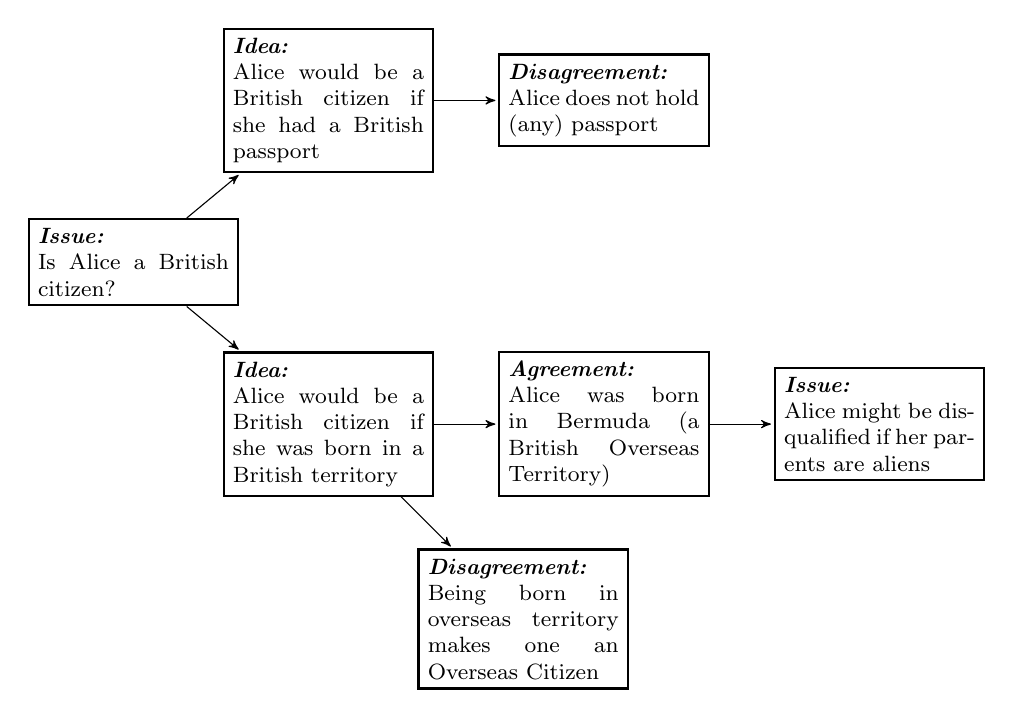
\begin{tikzpicture}[node distance=3.5cm,>=stealth',bend angle=10]

	\tikzstyle{rect}=[
		rectangle,
		thick,
		draw=black,
  		fill=white
  	]
	

	\node [rect, font=\footnotesize] (A) [] {\parbox{0.2\textwidth}{\textbf{\textit{Issue:}}\\Is Alice a British citizen?}};

	\node [rect, font=\footnotesize] (B) [above right=16mm] {\parbox{0.2\textwidth}{\textbf{\textbf{\textit{Idea:}}}\\Alice would be a British citizen if she had a British passport}};
	\node [rect, font=\footnotesize] (C) [below right=16mm] {\parbox{0.2\textwidth}{\textbf{\textit{Idea:}}\\Alice would be a British citizen if she was born in a British territory}};
	

	\node [rect, font=\footnotesize] (E) [right of=B] {\parbox{0.2\textwidth}{\textbf{\textit{Disagreement:}}\\Alice does not hold (any) passport}};
	
	\node [rect, font=\footnotesize] (F) [right of=C] {\parbox{0.2\textwidth}{\textbf{\textit{Agreement:}}\\Alice was born in Bermuda (a British Overseas Territory)}};
	\node [rect, font=\footnotesize] (G) [below right of=C] {\parbox{0.2\textwidth}{\textbf{\textit{Disagreement:}}\\Being born in overseas territory makes one an Overseas Citizen}};
	
	\node [rect, font=\footnotesize] (H) [right of=F] {\parbox{0.2\textwidth}{\textbf{\textit{Issue:}}\\Alice might be disqualified if her parents are aliens}};
	
	\draw[post] (A)--(B)  ;
	\draw[post] (A)--(C)  ;
	
	\draw[post] (B)--(E)  ;
	
	\draw[post] (C)--(F)  ;
	\draw[post] (C)--(G)  ;
	
	\draw[post] (F)--(H)  ;
      
\end{tikzpicture}
\end{center}
\caption{Example usage of an IBIS model, examining whether Alice is a British citizen}
\label{figure:ibis}
\end{figure}


\subsubsection{Wigmore's Chart}
``Wigmore's chart'', conceived in 1913, is a means of recording argumentation originally devised for use in legal trials. The chart models the chain of interactions between competing arguments from both participants and can be used to evaluate the overall conclusion that should be drawn \citep[p.~751]{Wigmore1913}. It takes the form of a directed graph where each node represents a particular fact. The shape of each node relates to the nature of the assertion; squares represent testimony given under oath; a triangle represent an explanation of or support for the node it ``points'' to; an open angle refutes the argument it points to and all other assertions (such as claims, physical evidence or related legal statutes) are represented by circles. These can additionally be marked to denote arguments by the defence or prosecution, but are not discussed here for clarity \citep{Chalamish2011, Chalamish2013}. Symbols relate further information about the nature of these assertions: an infinity symbol ($\infty$) states that a node denotes sensory evidence that may be (re)produced in court; a pilcrow (\P) denotes an assertion that can be taken as fact with no further evidence (such as a precedence case); a lack of a symbol shows that the claim is implied from further reasoning in the graph. In addition, Wigmorean analysis can incorporate the notions of \textit{strong belief} ($\bullet\bullet$), \textit{belief}($\bullet$) \textit{doubt} (?) \textit{disbelief} ($\circ$) and \textit{strong disbelief} ($\circ\circ$) (\citealp[p.~751-756]{Wigmore1913}; \citealp{Goodwin2000}). Little is known about precisely how often this type of analysis is used manually, although it is thought that it is carried out in courthouses around the world \citep{Chalamish2011}. However, efforts are being made to automate the process by parsing the natural language propositions made in court and transforming these into a Wigmore diagram to aid judges, barristers and juries in their deliberations \citep{Chalamish2013}.

\begin{figure}[h!]

\makeatletter
\newif\ifpgfshapebaselesstrianglehasinline
\newif\ifpgfshapebaselesstriangleclose
\pgfkeys{/pgf/.cd,
  baseless triangle apex angle/.style={/pgf/isosceles triangle apex angle=#1},
  baseless triangle inline/.is if=pgfshapebaselesstrianglehasinline,
  baseless triangle has base/.is if=pgfshapebaselesstriangleclose
}

\pgfdeclareshape{baseless triangle}{
  % Copy some stuff from the isosecles triangle
  \inheritsavedanchors[from={isosceles triangle}]
  \inheritanchor[from={isosceles triangle}]{center}
  \inheritanchor[from={isosceles triangle}]{north}
  \inheritanchor[from={isosceles triangle}]{south}
  \inheritanchor[from={isosceles triangle}]{east}
  \inheritanchor[from={isosceles triangle}]{west}
  \inheritanchorborder[from={isosceles triangle}]
  \backgroundpath{%
    % The isoceles triangle defines lots of parameters
    % in the \trianglepoints macro.
        \trianglepoints%
        {%
            \pgftransformshift{\centerpoint}%
            \pgftransformrotate{\rotate}%
            % This bit is a bit of a kludge to ensure the inline
            % is at the top of the figure.
            \pgftransformyscale{cos(\rotate)}%
            \pgfpathmoveto{\lowerleft}%
            \pgfpathlineto{\apex}%
            \pgfpathlineto{\lowerleft\pgf@y=-\pgf@y}%
            % Close the base?
            \ifpgfshapebaselesstriangleclose%
              \pgfpathclose%
            \fi%
            % Draw the inline?
            \ifpgfshapebaselesstrianglehasinline
              \pgfpointdiff{\lowerleft}%
                 {\pgfpointlineattime{0.125}{\lowerleft}{\lowerleft\pgf@y=-\pgf@y}}%
                \pgfgetlastxy{\x}{\y}%
                \pgfmathveclen{\x}{\y}%
                \let\inlineshift=\pgfmathresult%
            % Calculate where the inline hits the sloped line of the triangle.
            \pgfmathparse{\inlineshift/2/sin(\pgfkeysvalueof{/pgf/isosceles triangle apex angle}/2)}%
            \let\inlineendshift=\pgfmathresult
            \pgfpathmoveto{\pgfpointadd{\pgfpoint{0pt}{-\inlineshift}}{\lowerleft}}%
            \pgfpathlineto{\pgfpointlineatdistance{\inlineendshift}{\apex}{\lowerleft}\pgf@y=-\pgf@y}%
        \fi%
    }
    }
}

\begin{center}
\begin{tikzpicture}[node distance=1.6cm,>=stealth',bend angle=45]

	\tikzstyle{circ}=[
		circle,
		thick,
		draw=black,
		fill=white,
		minimum size=6mm
	]

	\tikzstyle{rect}=[
		rectangle,
		thick,
		draw=black,
  		fill=white,
  		minimum size=6mm
  	]
  			  
	\tikzset{
		support/.style={
			regular polygon,
			regular polygon sides=3,
			shape border rotate=90,
			thick,
        	draw=black,
	        fill=white,
        	minimum height=6mm,
        	node distance=0.6cm
    	}
    }
    
    \tikzset{	
		refute/.style={
	    	draw,
	    	thick,
	    	baseless triangle,
 	   		baseless triangle apex angle=60,
 	   		shape border rotate=180,
 	   		baseless triangle inline=false,
 	   		baseless triangle has base=false,
 	   		node distance=0.6cm
  		}
  	}



	\node [circ,tokens=1] (1) [label=above right:$_1$] {};
	
	\node [circ,tokens=2] (2) [right of=1,label=above right:$_2$,label=below right:$\infty$] {};
	\node [support] 	  (2a)[left of=2] {};	
	
	\node [circ,tokens=1] (3) [below left of=1,label=above right:$_3$] {};	
	\node [circ,tokens=2] (4) [below of=3,label=above right:$_4$,label=below right:\footnotesize{\P}] {};

	\node [circ,tokens=1] (5) [below right of=1,label=above right:$_5$] {};
	


	\node [rect,tokens=1] (6) [below of=5,label=above right:$_6$] {};	

	\node [circ] (7)  [right of=6,label=above right:$_7$] {$\circ$};
	\node [refute] (7a)  [left of=7] {};

	\draw[post] (3)-|(1)  ;
	\draw[post] (5)-|(1)  ;
	\draw[post] (4)--(3)  ;
	\draw[post] (6)--(5)  ;
	\draw[post] (2a)--(1)  ;
	\draw[post] (7a)--(6)  ;
	
 
      
\end{tikzpicture}
\end{center}

\begin{tabular}{l l}
\begin{minipage}{0.5\textwidth}
\begin{enumerate}
	\item[$^1$] \footnotesize{Alice is a British citizen}
	\item[$^2$] \footnotesize{Alice has a British passport}
	\item[$^3$] \footnotesize{A person born in a British territory will be a British citizen}
	\item[$^4$] \footnotesize{British Overseas Territories Act 2002}
\end{enumerate}
\end{minipage}

\begin{minipage}{0.5\textwidth}
\begin{enumerate}
	\item[$^5$] \footnotesize{Alice was born in Bermuda}
	\item[$^6$] \footnotesize{Alice's parents testify that she was born in Bermuda}
	\item[$^7$] \footnotesize{Alice's parents' testimony could be biased in her favour}
\end{enumerate}
\end{minipage}
\end{tabular}
\caption{Example Wigmore graph, examining whether Alice is a British citizen}
\label{figure:wigmore}
\end{figure}


\subsubsection{Dung's Framework}
Similar to Wigmore's method, Dung's framework (which uses the format of set theory) focuses on the aspect of arguments attacking, (implicitly) supporting and, ultimately, defeating one another \citep{Dung1995}. Dung defines an \textit{Argument Framework} as a pair such that $AF = \langle AR, attacks \rangle$ where $AR$ is a set of arguments $\left\{a_1, a_2, ..., a_n\right\}$ and $attacks$ is a binary relation such that $attacks \subseteq AR \times AR$. $attacks$ describes which arguments are ``defeated'' by one another: for example, if $a_1$ is the argument ``Alice is not a British citizen'' and $a_2$ is the argument ``Alice has a British passport'' then $(a_2, a_1) \in attacks$. The set of \textit{conflict free} arguments is a maximal set of arguments that do not attack each other. An argument $a_1$ is \textit{acceptable} with regard to a set of arguments $S$ if there is no argument $a_2$ that attacks $a_1$ that is not itself attacked by an argument in $S$. A set of arguments is \textit{admissible} if each argument is considered \textit{acceptable} with respect to the set. The maximal \textit{admissible} set is known as a \textit{preferred extension} \citep{Schneider2013}. 

\TODO{Other extensions}
There have been a number of extensions to this framework.
\citet{Bench-Capon2002} have extended this framework to incorporate the idea of ``value'' or principle to arguments. When circumstances arise such that two possible resolutions to a dispute are equally (logically) valid, different audiences will have differing preferences based on the principles they feel are most important. For example, say that two solutions for combating crime are put forward: reading the general public's private correspondence or an expensive social program of education and rehabilitation. If each has been proven to be equally effective, audiences that value minimisation of cost may favour the former whereas audiences that value individual privacy might choose the latter.
\citet{dunne2016heard} incorporated this to \TODO{FINISH}


\subsubsection{ASPIC}
\TODO{EXPAND THESE}

\subsubsection{ASPIC+}

\subsubsection{IMPACT structured consultation tool}
\TODO{THIS} \citep{wyner2011towards}

\subsubsection{The Argument Interchange Format}
The Argument Interchange Format (AIF) is a framework for representing argumentation as a directed graph \citep{Chesnevar2006}. Created as part of the Argument Web project \citep{Rahwan2007a}, which aims to link the concepts of natural language argumentation with abstract mathematical modelling (including capturing \textit{``linguistically sophisticated manoeuvres''} \citep{Bex2013}), the AIF is primarily a description, with specifications in a number of languages including RDF and SQL.

At its highest level, the AIF can be conceptually divided into an ``upper'' ontology and a ``forms'' ontology. The upper ontology consists of the building blocks of the argument structure, while the forms ontology applies context, for example, by differentiating between logical attacks based on faulty evidence, witness bias, or appeals to authority. The data, claims and conclusions that make up the argument are modelled by Information nodes (I-nodes). There can be no direct relationship between I-nodes. Instead, there must be an intermediary Scheme node (S-nodes). These S-nodes are subdivided into three applications: Rule of Inference Applications (RA-nodes), Conflict Applications (CA-nodes) and Preference Applications (PA-nodes). RA-nodes and CA-nodes simply denote an inference or conflict (logical or otherwise) between one or more pieces of information. PA-nodes, however, denote a preference of one piece of information over another. For example when discussing economics, while it may be difficult to logically prove the superiority of a regulated market over a free market, or vice-versa, the personal beliefs and preferences of proponent and opponent will feature heavily in their reasoning on such issues \citep{Bench-Capon2002}. This structure is displayed in Figure \ref{figure:ontologies:aif}.

\begin{figure}
\begin{center}
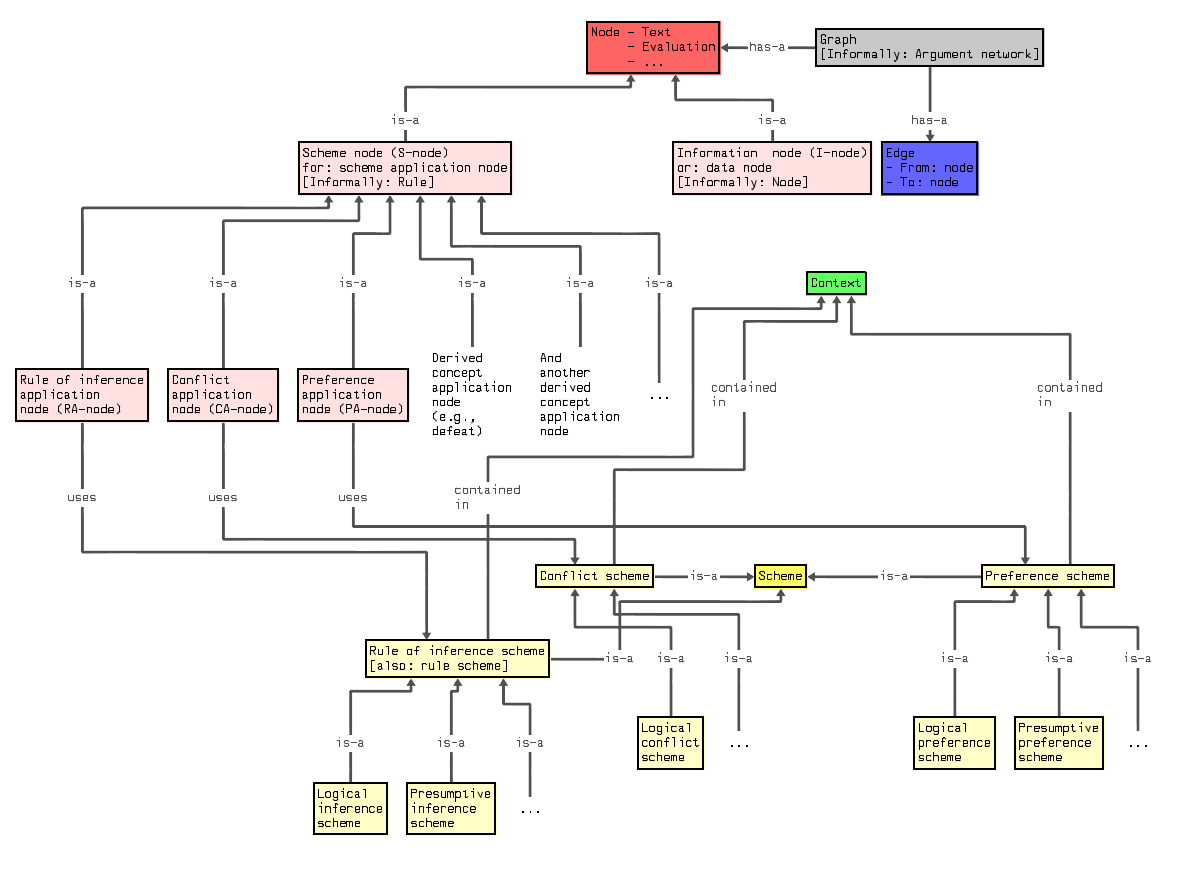
\includegraphics[scale=0.42]{./figures/ontologies/aif.png}
\caption{An overview of the AIF Ontology \citep{Chesnevar2006}}
\label{figure:ontologies:aif}
\end{center}
\end{figure}

\subsubsection{AIF+ and Inference Anchoring Theory}

\TODO{Expand details from IAT paper}


In their work on an extension to the AIF, dubbed the AIF+, Reed et al. build on the work of O'Keefe to differentiate between two separate notions of argumentation \citep{Benoit1992, Reed2008}: the first, which they term argument$_1$, is a logically constructed set of claims and evidence used to back these claims (or attack other claims), as in \textit{``Alice put forward her argument''}. The second, termed argument$_2$, refers to a dialogue -- the exchange of ideas and opinions between two or more people, as in \textit{``Alice and Bob were having an argument}. A result of this work was to introduce a new set of nodes. The first, a subset of I-nodes dubbed Locutions (L-nodes), model locutionary acts (or utterances) in an argument$_2$. That is, they record precisely what was said. The second, a subset of S-nodes dubbed Transition Applications (TA-nodes), represent transitions between L-nodes (with associated forms such as a challenge or response). Thirdly Illocutionary Applications (YA-nodes), also a subset of S-nodes, represent the ``illocutionary force'' and serve to link each argument$_1$ to the overall argument$_2$. Figure \ref{figure:graphs:aifplus} shows how this structure can be visualised. Consider the locution \textit{``All men are mortal, and Socrates is a man. Therefore, Socrates is mortal.''} The statement itself is modelled using the L-node on the rightmost side of the diagram. On the leftmost side is the core AIF structure, which show the premises formed as two I-nodes (\textit{``Socrates is a man''} and \textit{``All men are mortal''}), linked to the conclusive I-node (\textit{``Socrates is mortal''}) by way of an RA-node. The L-node is connected to this argument$_1$ by way of the YA-node, shown in the middle.

\begin{figure}
\centering
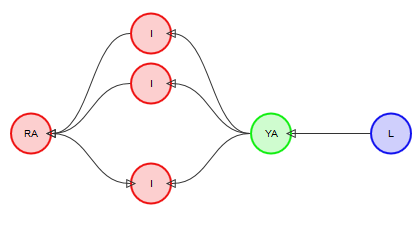
\includegraphics[scale=0.5]{./figures/graphs/aifplus.png}
\caption{Visualisation of a simple AIF+ graph}
\label{figure:graphs:aifplus}
\end{figure}

\section{Online Communication and Interaction}
\label{background:online}

\subsection{Social Media and the Social Web}
\label{background:online:social}
The social web consists of the people, tools and communities that form over the world wide web, and is a way for individuals to share content, ideas and information. The social web presents a number of challenges for extracting and analysing arguments, particularly due to the lack of clear ``indicators'' of argument or structure. This problem is compounded by the type of language used; often highly informal, incorporating slang and irregular punctuation and grammar \citep{Schneider2012}. As the social web becomes more and more ubiquitous, the potential for using it to investigate how truly massive communities interact, communicate and argue increases dramatically.

Many theoretical models of argumentation are based on the assumption of a dialectic argument, as their purpose is to aid the participants with the process of understanding the information discussed, or to reason over the model and draw conclusions regarding the outcome. However, in social media there is a clear proliferation of eristic argumentation \citep{sood2012automatic}. This makes the role of audience an important feature to consider: when an individual responds to a post on the social web their post is often seen not just by the author of the post they reply to, but by many other users as well. In fact, many posts may be directed at this wider audience to seek approval, voice dissent, or provoke other emotions \citep{berland2010students}. Consider the analogy of a political hustings: neither candidate believe they can change the mind of their opponent, but instead are debating with a view to sway their audience. Schneider et al. note though, that currently it is difficult to model the value of eristic arguments as participants are free to \textit{``sling propositions that they would not commit to under other circumstances''} as a means of catharsis, recreation or entertainment \citep{Schneider2014}.

\citet{Kaplan2010} classify six distinct categories of social media: collaborative projects, blogs, content communities, social networking sites, virtual game worlds and virtual social worlds. Collaborative projects allow many different users to create, maintain and often discuss content. This category includes sites such as the online encyclopaedia \textit{Wikipedia}\footnote{https://en.wikipedia.org/}, which allow users to write and edit articles and \textit{Urban Dictionary}\footnote{http://urbandictionary.com/‎}, a user generated dictionary of slang and internet culture. \citeauthor{Kaplan2010} compare blogs (web-logs) to personal websites, in that they allow users to post information about the subject of their choice -- these posts are often timestamped and presented reverse-chronologically. \textit{Wordpress}\footnote{http://wordpress.com/} and \textit{Blogger}\footnote{http://blogger.com} are two social media sites specialised for this purpose. ``Micro''-blogging sites that pose limits on the amount of content that can be shared in a single post, such as \textit{Twitter}\footnote{http://twitter.com/}, also fall into this category. Content communities revolve around the concept of publishing (and ultimately sharing) different forms of media. These include sites for publishing video (such as \textit{Vimeo}\footnote{http://vimeo.com/}), images (such as \textit{Flickr}\footnote{http://flickr.com/}), audio (such as \textit{SoundCloud}\footnote{http://soundcloud.com/}) and many other different types of media. Social networking sites allow users to create a profile detailing information about themselves (such as home town, or music preferences) and then connect their profiles with the profiles of others on the site. Examples include \textit{Facebook}\footnote{http://facebook.com} and \textit{Google+}\footnote{http://plus.google.com/}. Virtual game worlds (such as \textit{World of Warcraft}\footnote{http://battle.net/wow/}) encompass online games in which a user controls a digital avatar to accomplish certain tasks (such as slaying a virtual dragon, or defeating another player's avatar). Similarly, virtual social worlds (such as \textit{Second Life}\footnote{http://secondlife.com}) encompass virtual spaces in which users have an avatar, but there is no specified aim or end-goal -- the medium exists solely to facilitate social interaction. In this work, less focus is afforded to these latter two areas of the social web due to the the issue that as participants are controlling a virtual avatar, and may be playing a particular ``role'' rather than their real self, this can affect their behaviour and engagement in a discussion \cite{Hooi2013}. There is also the tendency for discussions to centre on the mechanics of the game world itself \citep{alagoz2013}.

\subsection{Anti-Social Behaviour}
\label{background:online:antisocial}
Anti-social behaviour is a growing problem on the social web, and often arises from debates or discussions that get out of hand \citep{suler1998bad, davis2002experience, sood2012automatic}. This behaviour can arise from simple misunderstandings due to the difficulty in conveying tone through text, or as a deliberate act by individuals lashing out at other participants in a discussion. Incidents include
flaming, in which a user simply hurls emotional abuse \citep[p.~13]{Konijn2008}; spamming, in which a user floods the medium with content, often unrelated to the topic in hand, in the hope of drowning out other participants or as a means of advertising a commercial product \citep{krause2008anti}; trolling, in which a user posts seemingly innocuous but deliberately fallacious argument to provoke other members of the group into becoming outraged (although there is debate as to whether this term refers to the bridge-dwelling monster of myths, or the fishing term for dangling a baited line behind a boat) \citep{Herring2002}; 
and much more serious incidents of directed threats and stalking \citep{spitzberg2002cyberstalking, willard2007, jane2014}.

As a result, there is a concerted research effort into the best way to tackle these issues before they cause serious harm to individuals, or the field as a whole. \citet{suler1998bad} discuss a wide variety of approaches (specifically in regard to the virtual social world \textit{The Palace}\footnote{http://thepalace.com}, but these could be applied to other online spaces as well). The simplest solution is to moderate users' interactions and dispense warnings, ``mutes'' (where a user may observe, but not contribute) or, in extreme cases, bans as and when the situation warrants. While effective for dealing with small or close-knit communities, this approach does not scale when considering the social web.

\TODO{Arguments against the troll} \citep{torroni2010}

A different approach is to allow the community a degree of self-moderation. Reputation systems, for example, allow users within a community to assign ``votes'' to a particular account, or post, to show its trustworthiness. This allows new users to make judgements on whether to take a comment seriously, for example, or to purchase something from a particular seller in an online auction \citep{resnick2000reputation, anderson2012discovering}. However, this can also lead to a feedback loop in which communities become self-reinforcing; if users always vote for posts of similar sentiment (or against those that disagree), then gradually these sentiments will become dominant. Over time only users who hold these views will contribute to the site (further reinforcing the disparity) and the community as a whole will stagnate or worse, become distrustful or outright hostile to new members or ``outsiders''.

In another example of direct self-moderation, the popular online game \textit{League of Legends}\footnote{http://leagueoflegends.com} implements a ``tribunal'' system in which players that are reported for poor behaviour in matches (such as verbally abusing team-mates) are judged by their peers. These peers can examine evidence such as chat logs and game scores, then decided whether to ``pardon'' or ``punish'' the offending player \citep{Hodson2013, kou2013regulating}.

A more covert attempt to manipulate users' behaviour can be found in certain implementations of human-computer interaction design. HCI can be leveraged to ``trick'' users into performing (or not performing) an action desirable to the designer. These so-called ``malicious interfaces'' \citep{Conti2010} are often used to trick users into spending time or money that they otherwise would not (for example, advertising banners that suddenly cover page content). In 2008, YouTube temporarily added an ``Audio Preview'' button to its comment system that would read aloud what the user intended to post. This was placed in the previous place of the ``post'' button (which had been moved further to the right), such that a user was likely to unintentionally preview their comment before posting it \citep{Munroe2008}.


\subsection{Semantically-Interlinked Online Communities}
%\TODO{Find some more models?}
The Semantically-Interlinked Online Communities project (SIOC) aims to enable the cross-platform, cross-service representation of data from the social web \citep{Breslin2006}. SIOC allows for semantic representations of Sites, which hold Forums, which contain Posts, authored by the owner of a UserAcount. This structure is shown in Figure \ref{figure:sioc}. SIOC is often used in conjunction with the Friend of a Friend (FOAF) ontology, to show how individuals map to their online personas.

\begin{figure}
\begin{center}
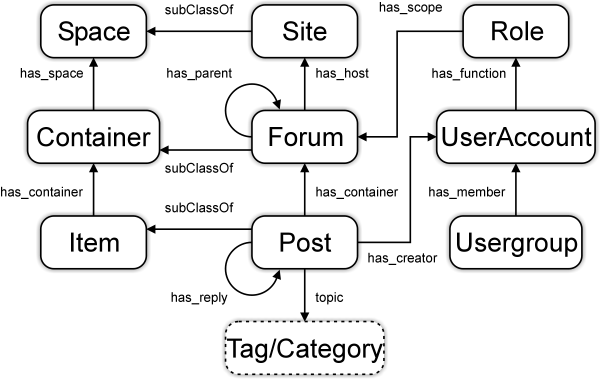
\includegraphics[scale=1.75]{./figures/ontologies/sioc.png}
\caption[An overview of the core SIOC ontology]{An overview of the core SIOC ontology\protect\footnotemark}
\label{figure:sioc}
\end{center}
\end{figure}
\footnotetext{http://sioc-project.org/ontology}

While an extension to SIOC, for the purposes of capturing and representing argumentation, does exist \citep{Lange2008}, it is based on the Issue Based Information System (IBIS) principals of modelling an argument as an issue that needs to be solved, with users suggesting ideas, then providing arguments for or arguments against these ideas. While this approach is highly useful when dealing with arguments centred around deliberation, and to a lesser extend criticism or inquiry, they are not as suitable when modelling negotiations or eristic arguments.

\section{Social Aspects of Argumentation}
\TODO{ReasonWell, etc.}

\TODO{Prescriptive vs. Descriptive etc.}

\section{Summary}
\TODO{Summarise}
\chapter{Preliminary Investigation into Modelling with the AIF}
\label{investigation}
To determine how capable current tools and frameworks are for capturing social argumentation, and the nuances between dialectic and eristic argumentation, a preliminary investigation was conducted. This aimed, firstly, to show how these tools and frameworks can be combined in a way that makes them fit for this particular purpose and, secondly, to determine the key strengths and weaknesses of this combination in relation to modelling social argumentation.


\section{Approach}
The AIF was determined to be the closest fit for purpose ontology for modelling argumentation on the social web, due to the goals of capturing practical, language-based argumentation, with the additional benefit of being readily extensible. Alongside the SIOC, the key elements of these ontologies have been combined to explicitly capture the social component of argumentation on the social web, while also modelling the formalised argument structure. This is achieved by linking the concept of a SIOC Post with that of an AIF Locution, treating a social web thread as a separate dialogue, or argument$_2$ and each post as an atomic unit within the dialogue (containing zero or more individual arguments$_1$). In the majority of cases, a single locution will translate to a single self-contained argument$_1$. However, a single post can contain a number of arguments$_1$ -- each with a number of premises and a single conclusion. In this situation a single L-node will link to multiple YA-nodes, as shown in Figure \ref{figure:graphs:aswo-multiple-ya}. In rare cases (often caused by constraints imposed on the length of a post by the service, such as the 140 character limit on Twitter), a user will spread the premises of a single argument across multiple posts to construct their argument$_1$. Figure \ref{figure:graphs:aswo-single-ya} shows how, in such a situation, multiple L-nodes will link to a single YA-node. If two users post identical statements, they still contribute two distinct locutions. However, they will both be linked to the same I-node(s), and therefore the same argument$_1$. In this situation, multiple YA-nodes may point to the same I-node, such as in Figure \ref{figure:graphs:aswo-repeated-argument}.


\begin{figure}
\centering
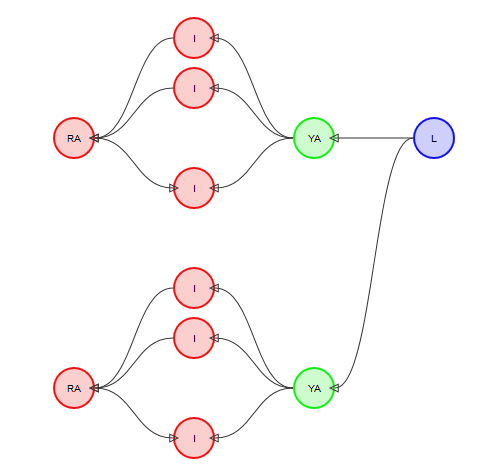
\includegraphics[scale=0.5]{./figures/graphs/aswo-multiple-ya.png}
\caption{Visualisation of one post making two distinct arguments$_1$}
\label{figure:graphs:aswo-multiple-ya}
\end{figure}


\begin{figure}
\centering
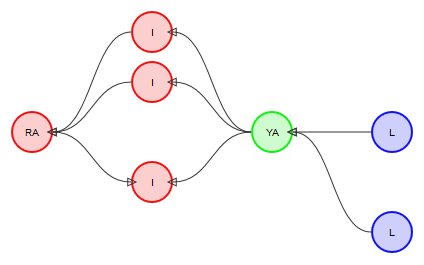
\includegraphics[scale=0.5]{./figures/graphs/aswo-single-ya.png}
\caption{Visualisation of two posts, used to construct a single argument$_1$}
\label{figure:graphs:aswo-single-ya}
\end{figure}


\begin{figure}
\centering
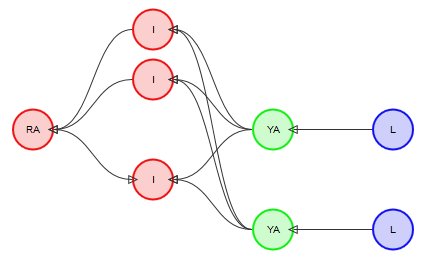
\includegraphics[scale=0.5]{./figures/graphs/aswo-repeated-argument.png}
\caption{Visualisation of two posts, repeating the same argument$_1$}
\label{figure:graphs:aswo-repeated-argument}
\end{figure}


\section{Methodology}

\subsection{Data Collection}
\label{investigation:methodology:datacollection}
A single topic of argumentation was chosen to be examined for three case studies, each representing a different social media system. To ensure the stimulation of debate, the selected topic needed to be controversial, have a large number of respondents and have been active for a long enough period of time to generate a rich and complete content. The October 2013 United States government shutdown caused by Congress's failure to agree on a budget, and the following condemnation this received from the presidency, was a suitable match for these requirements. 

This topic was then tracked across three of the social media categories identified by \citet{Kaplan2010}: Twitter, a microblogging service that allows users to publish messages of up to one-hundred and forty characters; Facebook, a social network, that allows users to create a network of ``friends'' and share text or images; and YouTube, a content creation site where users can create and upload videos, or playlists of videos.

The source of the posts themselves again needed to be both publicly available and have a large number of followers to ensure a maximally stimulated debate. As an authoritative public figure at the heart of the crisis, content from or relating to Barack Obama's social media profiles was chosen, and three posts that were broadly similar in content were selected for study. The first post, initially posted on 8th October 2013 from the White House's YouTube channel\footnote{https://www.youtube.com/watch?v=7LwoudGfug0}, is a 14m 40s video recording of Obama delivering a statement to press from the West Wing of the White House, condemning the shutdown. The post taken from Obama's official Twitter account\footnote{https://twitter.com/BarackObama/status/390288744235823104} (which is managed by a third party, Organizing for Action), dated 15th October 2013, reads: \textit{``This is unacceptable. Tell Tea Party Republicans to stop holding our economy hostage: http://OFA.BO/qNmA3Y''}. The included hyperlink leads to an Organising for Action page, which encourages users to to voice their displeasure at the shutdown by allowing them to automatically generate and send tweets. The post taken from Obama's official Facebook account\footnote{https://www.facebook.com/photo.php?fbid=10151874920756749} (also managed by Organizing for Action), also dated 15th October 2013, reads: \textit{``Tea Party Republicans in the House of Representatives forced a government shutdown, and now they're threatening an economic shutdown. This has gone on for too long. Tell them to \#EndThisNow: http://OFA.BO/ACC7qB''}.

The discussions surrounding these posts were acquired by collecting comments replying to each initial post, and those replying to subsequent posts in the discussion (taking into account only direct replies, rather than mentions within the text of the post), with the use of the public Twitter, Facebook and Youtube APIs respectively. This data was translated to an RDF triple-store using SIOC to record the data specific to the social media platform, such as which User created which Post and which Thread stores which Posts. This was used in conjunction with the DCTerms ontology, which held supplementary data such as timestamps.

\begin{table}
\centering
\caption{Metrics of total dataset collected from YouTube, Twitter and Facebook}
\label{table:results:totalstats}
\begin{tabular}{ l | r  r  r }
\textbf{Metric} & \textbf{YouTube} & \textbf{Twitter} & \textbf{Facebook} \\
\hline
Total number of posts 				& 2719 & 137 & 9494 \\

Total number of users 				& 1255 & 33 & 6224 \\

Average posts per user 				& 2.17 & 4.15 & 1.53 \\

Average words per post 				& 26.74& 15.91 & 40.12  \\

Average characters per post 		& 150.13 & 97.63 & 241.14 \\

Time between first and last posts 	& 101d 16h 19m 12s & 0d 13h 40m 48s & 90d 19h 55m 12s\\

Average time between posts			& 53m 52s & 3m 02s & 13m 47s \\

\end{tabular}
\end{table}


\subsection{Data Sampling and Annotation}
\label{method:annotation}
Because of the volume of the data produced over the course of the tracked event and the time-intensive nature of manually annotating the data, it was necessary to sample the data to a more manageable size before annotation could take place. To prevent information being lost when the dataset was scaled down, it was important to  ensure that the sampled graph maintained properties (such as diameter and average path length) similar to those of the raw data. To maintain these characteristics, ``forest fire'' sampling \citep{leskovec2005graphs, leskovec2006sampling} was used to create a sub-graph that preserved the overall structure of the parent. The algorithm for forest fire sampling is as follows:
\begin{enumerate}
\item Choose a ``forward burning probability'' $p$ -- in this instance a value of 0.7 was chosen based on the recommendation by \citet{leskovec2006sampling} for scaling down a larger graph

\item Choose a random starting node
\label{enum:forest-fire:start}

\item Add this node to the sample graph. Select $x$ nodes at random from all nodes linked to the chosen node, where $x$ is a random number geometrically distributed with mean $\frac{p}{1-p}$. If the selected node has fewer than $x$ linked nodes, select all available nodes, and return to step \ref{enum:forest-fire:start}.
\label{enum:forest-fire:recurse}

\item With each selected node, recursively repeat step \ref{enum:forest-fire:recurse} until the desired sample size has been reached. 
\end{enumerate}

Thirty posts from within the following discussion (i.e. not including the original posts) were selected using this method. This data was then manually annotated with the formal argument$_1$ information. Specifically, from each L-node, both explicit and implicit I-nodes were extracted and related together using the most appropriate S-nodes. %For example, Obama's original Twitter post (an L-node) states: \textit{``This is unacceptable. Tell Tea Party Republicans to stop holding our economy hostage: http://t.co/y8fPF8s3bG''}. From this the following I-nodes can be extracted: \textit{``The Tea Party Republicans are holding the economy hostage''}, \textit{``Holding the economy hostage is an unacceptable tactic''} and \textit{``The Tea Party Republicans should stop holding the economy hostage''}. From this, it is easy to see that the single locution contains two premises and a conclusion (which therefore need to be joined using an RA-node). This argument$_1$ can then be mapped to the specific locution by means of a YA-node.

\begin{table}
\centering
\caption{Metrics of discussions sampled from YouTube, Twitter and Facebook}
\label{table:results:samplestats}
\begin{tabular}{ l | r r r r }

\textbf{Metric} & \textbf{YouTube} & \textbf{Twitter} & \textbf{Facebook} & \textbf{All}\\
\hline
Total number of posts & 30 & 30 & 30 & 90\\

Total number of users & 23 & 12 & 30 & 65\\

Average posts per user & 1.30 & 2.50 & 1.00 & 1.38\\

Average words per post & 26.77 & 16.33 & 42.10 & 33.18\\

Average characters per post & 147.90 & 101.20 & 259.67 & 201.70\\

Time between first and last posts & 4d 0h 54m 56s & 0d 5h 13m 33s & 3d 12h 13m 18s & n/a\\

Average time between posts & 3h 20m 31s & 0h 10m 49s & 2h 54m 15s & 0h 17m 10s\\

\end{tabular}
\end{table}

\section{Results and Analysis}
\label{investigation:results}
An overview of the raw data collected from each platform is shown in Table \ref{table:results:totalstats} and the sampled data in Table \ref{table:results:samplestats}. In total, the discussion generated by the Twitter post has slightly over one-hundred and thirty replies -- in contrast, the  YouTube comments total nearly three thousand posts, and the Facebook discussion has well over nine-thousand. Each platform sees the vast majority of posts contributed soon after the initial post. However, each has a ``long tail'' of responses that gradually decrease in frequency as time goes on. The discussion on Twitter seems particularly ephemeral, with participants only contributing for a short time before moving onto other topics; while the Facebook and YouTube posts appear more ``permanent'', with users finding and contributing to them months later.

\begin{table}
\centering
\caption{Aspects of raw data from social media APIs capable of being modelled using the AIF or SIOC ontologies}
\label{table:method:features}
\begin{tabular}{ r | c | c }

\multirow{2}{*}{\textbf{Features present in social media APIs}} & \multicolumn{2}{c}{\textbf{Represented in:}}\\

 & \textbf{AIF} & \textbf{SIOC} \\
\hline
Locution (explicit content)& $\checkmark$ & $\checkmark$ \\

Illocution (premises/conclusions) & $\checkmark$ & \\

Argumentation structure (attacks/support) & $\checkmark$ & \\

Author  		& $\checkmark$ & $\checkmark$ \\

Avatar  		&  			   & $\checkmark$ \\

Replies 		& $\checkmark$ & $\checkmark$ \\

Creation Date  	& $\checkmark$ & $\checkmark$ \\

Reputation (e.g. ``Likes'')  &  &  \\

Location  &  &  \\

User ``Type'' (i.e. individual/business/etc.)  &  &  \\

Sentiment (implicit content) &  &  \\

\end{tabular}
\end{table}

In addition, when collecting this data it became apparent there was information that had no appropriate representation in either ontology, such as reputation systems (for example, the ``Likes'' used by Facebook), the sentiment of the post (for example, sarcasm, humour, abuse) or information about the type of user making the remark (whether they are an individual, a celebrity, a corporation, etc.); these omissions are shown in Table \ref{table:method:features}. These features could have substantial bearing on the perception of the argument$_2$. Consider the example of reputation systems: a retort stating \textit{``You're an idiot''} may be perceived very differently by the audience if it has no up-votes, one up-vote or one hundred thousand up-votes. Alternatively, consider a user making the argument$_1$ that \textit{``I really love using this product''}: whether the statement is made by an individual, or the company selling the product would likely influence the validity and value of the statement.

%\begin{figure}
%\begin{center}
%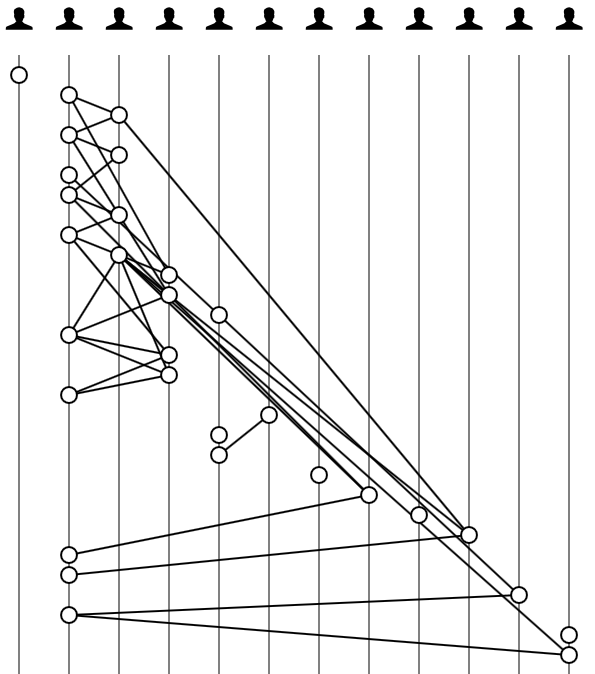
\includegraphics[scale=0.5]{./figures/lifelines_twitter.png}
%\caption{A subset of thirty Twitter replies, sampled using the forest-fire technique, visualised using Lifelines}
%\label{figure:lifelines-twitter}
%\end{center}
%\end{figure}

%\begin{figure}
%\begin{center}
%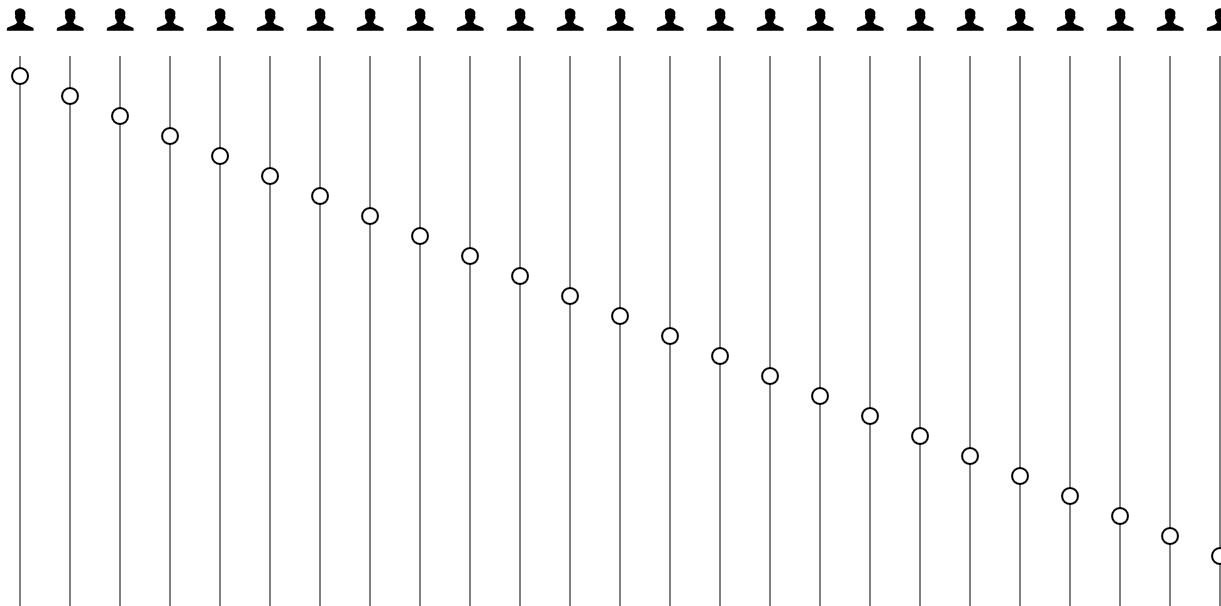
\includegraphics[scale=0.45]{./figures/lifelines_facebook.png}
%\caption{A subset of thirty Facebook comments, sampled using the forest-fire technique, visualised using Lifelines}
%\label{figure:lifelines-facebook}
%\end{center}
%\end{figure}

Table \ref{table:results:annotations} shows the statistics collected after annotating the data with premises and conclusions, represented as AIF nodes. Given this data it can be seen that Twitter is the only sample that contains Transition-nodes; that is, replies to other posts within the thread. While this may appear to suggest that the platform is used more fore debate than the others, it is possible this is down to deficiencies in the APIs of the other platforms, which often do not accurately highlight replies. It can also be observed that the debates on Twitter and Facebook have a much higher information content than that of YouTube. The resulting structures are visualised in Figure \ref{figure:speechacts}, which shows a side-by-side comparison of the three different samples.

\begin{table}
\centering
\caption{Summary of AIF nodes found in annotated discussions collected from YouTube, Twitter and Facebook}
\label{table:results:annotations}
\begin{tabular}{| l | c | c | c | c |}
\hline
\textbf{Metric} & \textbf{YouTube} & \textbf{Twitter} & \textbf{Facebook} & \textbf{Total} \\
\hline
L-nodes 			& 30	& 30 	& 30 	& 90\\
\hline
TA-nodes 			& 0		& 20 	& 0 	& 20\\
\hline
YA-nodes 			& 31	& 30	& 41 	& 102\\
\hline
I-nodes 			& 88	& 116	& 110 	& 314\\
\hline
S-nodes 			& 13	& 30    & 26 	& 69\\
\hline
L- to I-node ratio 	& 15:44	& 8:29  & 3:11	& 45:157\\
\hline
\end{tabular}
\end{table}

\begin{figure}
\centering
\begin{minipage}[b]{.30\textwidth}
  \centering
  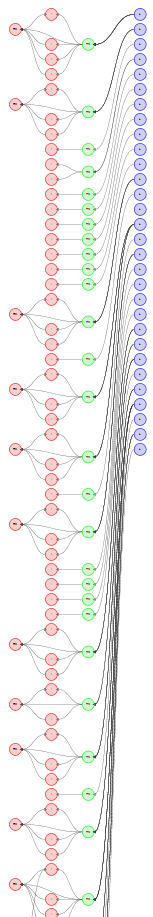
\includegraphics[scale=0.5]{./figures/speechacts/youtube.png}
\end{minipage}
\hspace{.05\textwidth}
\begin{minipage}[b]{.30\textwidth}
  \centering
  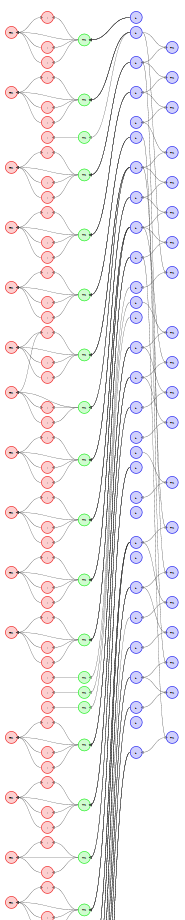
\includegraphics[scale=0.5]{./figures/speechacts/twitter.png}  
\end{minipage}
\begin{minipage}[b]{.30\textwidth}
  \centering
  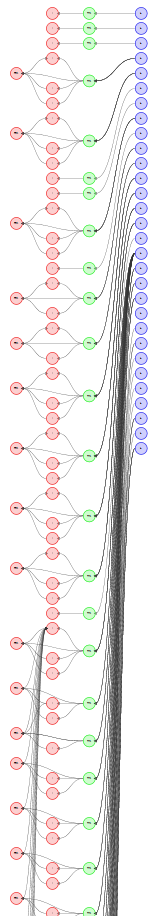
\includegraphics[scale=0.5]{./figures/speechacts/facebook.png}  
\end{minipage}

\caption{A side-by-side comparison of the emergent structures of discussions taken from YouTube (left), Twitter (centre) and Facebook (right)}
\label{figure:speechacts}
\end{figure}

On the surface, the sample of posts taken from Twitter and Facebook appear to have similar information content. However, upon manual inspection, it can be seen that this average is actually heavily skewed by one particular Facebook post that is thirteen paragraphs long and contains a total of twenty six information nodes. The argument in question is reproduced on a number of different websites, and is likely reused in full as a boilerplate ``cut and paste'' rebuttal by many users when engaging in an argument on that topic.

To highlight the overall information disparity take, for example, the tweet \textit{``@BarackObama Stop expanding government, spying on Americans and driving up the deficit.''}. This is an enthymeme -- the literally derived I-node acts as a conclusion, while the premises (that Obama is expanding government, spying on Americans and driving up the deficit  and that to do so is a bad thing) are left implicit. In turn, contrast with the posts \textit{``first''}, \textit{``wow obama''} and \textit{``lolollll i love this''} which contain very little information, either explicit or implicit. In addition, not all posts with a large amount of literal content have a comparatively large amount of information. For example, posts such as \textit{``Give DIRETIDE Give DIRETIDE Give DIRETIDE...''} (repeated upwards of fifty times in a single post) show a desire to derail the discussion by flooding it with completely irrelevant information (``Diretide'' refers to a cancelled seasonal event in the popular online game \textit{Defence of the Ancients 2}; the cancellation sparking uproar from the fanbase which led to a number of social media platforms being flooded with this message).

In addition, there are other posts that have deeper contextual meaning that would first appear. Consider, for example, ``RedScareBot''\footnote{https://twitter.com/RedScareBot}: this is an automated Twitter account that, using the avatar of Joseph McCarthy (an American politician famous for making claims at the height of the Cold War that their were numerous Soviet agents in the US government), replies to any tweet that includes phrases such as ``communism'' or ``commie'' with quips such as \textit{``Commie Chameleon''}, \textit{``Oh noes, Socialism''} or \textit{``Rise of the USSA''}. While this may seem nonsensical or a non-sequitur without context, \textit{with} context it can be viewed by the audience as a derisive or satirical retort to a knee-jerk insult, despite being posted by a machine.

There are of course limitations on the conclusions that can be drawn from a relatively small dataset when working with proverbial ``big data''. As such, these findings cannot be used to justify broad claims that state that \textit{all} arguments on a particular example of social media are structured in this way. These examples instead serve to demonstrate the important fact that different types of structures \textit{can} evolve, and provide some examples of the argumentative and rhetorical tactics people use when arguing over social media and how the conjunction of the AIF and SIOC projects (as well as any extensions made to these) can be used in attempts to map them.


\section{Summary}
\TODO{Summary}
\TODO{This shows that, currently, it is insufficient to use the AIF (and its extension) to fully model eristic argumentation, even when certain social aspects are  modelled through other ontologies such as SIOC.}
\chapter{The Argumentation on the Social Web Ontology}
\label{aswo}
In the preliminary investigation, the capability of existing frameworks and their use in capturing and modelling argumentation and social communities was examined and evaluated \citep{Blount2014}. It became apparent that the AIF, while a powerful tool for modelling (dialectic) argument, lacked the ability to capture the eristic aspects of social argumentation. While some logical fallacies, such as the \textit{ad hominem} attack can be suitably modelled within the AIF, the rhetorical force of ``simple'' abuse is difficult to capture. 

However, there is reason to suggest that while such abuse (for example) may not be valuable to the argument$_2$ itself, that does not mean it is not valuable to model such outbursts. A heckler in a debate, for example, may not have any well-reasoned argument$_1$ to hand and resort to throwing vulgarities, but by simply disrupting the proceedings they are voicing their dissent at the positions offered. This is reason enough not to discard the contribution; however, it can also act to catalyse further argumentation on the subject between the main participants. Likewise, a participant in a debate may, instead of putting forth their own argument or attacking their opponent's, make some sort of joke to endear themselves to the audience. While the AIF can model the locution, the rhetorical force behind it goes uncaptured.

In addition, there are other socio-rhetorical tactics that are often employed on social media. These include spamming (posting large volumes of a repetitive nature) to drown out other posters, deliberate deviation from the topic at hand, bringing up non-sequiturs in an attempt to derail the argument and ``meta-argumentation'' -- criticising the way in which an opponent argues, but not the argument itself (e.g. if a user claims another is breaking the rules of the forum, or of not arguing in good faith). There are also the non-textual features of social media to consider; that is, the feature of posts other than their content. For example, the number of ``Likes'' or ``Favourites'' a post has, demonstrates popular (or audience) support for this opinion or position. 


\section{Initial Proposals}
\label{aswo:augmentations}

\newcommand{\scaleProps}{0.7}

\TODO{Discuss different proposals, pros and cons, why settled on final choice}

%These results formed the basis for the work presented in the Workshop on Computational Models of Natural Argument, in which a number of suggestions on how these ontologies could be adapted to model the socio-rhetorical aspects of argumentation were proposed.

The principal focus here is the inclusion of rhetorical support and attack. While these features are only one aspect of rhetorical argument, they feature heavily in eristic dialogue (particularly rhetorical attacks), showcase both the positive and negative aspects of rhetorical argument and are important due to the impact they can have within discussions on the social web and the culture surrounding it \citep{Blount2015}.

Rhetorical support is often relatively benign. It can be used to show solidarity with other members of the dialogue, to incorporate oneself into a social group, or to encourage . Consider the extracts \textit{``bro fist bump''}, a short declaration of support for another user, and \textit{``I commend you for admitting that debt \& deficits are important...If only more [people] felt the way you do''}, which disagrees with the overall stance presented by their opponent, but commends them for conceding some common ground, in attempt to further dialectic argument.

Conversely, rhetorical attacks are often extremely hostile. They differ from logical attacks by attacking the person behind the argument rather than the argument itself (this is not to be confused with an \textit{ad hominem} argument which attacks a person's argument by calling their character or credentials into question -- these are logical, even though they are fallacious). Rhetorical attacks often contain extremely vulgar language.
%: consider the extracts \textit{``Some of you fucks need a good ass whipping''} and \textit{``Fuck off cunt''}. \TODO{Do I need to censor this?}
The purpose of these statements can be interpreted in a number of ways, from showing the audience how impassioned and emotive the rhetor is on the subject, to cathartically blowing off steam, to intentionally silencing dissenting voices with threats.

Figure \ref{figure:cmna:abuse1} shows the simplest approach, similar to the current way the AIF models the use of \textit{ad hominem} attacks, by linking the attack to the opponent's argument$_1$ with a CA-node. However, this is insufficient for the majority of abusive attacks; while \textit{ad hominem} tactics attack an opponent's argument$_1$ by claiming they are not qualified, or otherwise unfit, to make such an argument$_1$, abuse often does not attack their position at all, but seeks to undermine them emotionally in front of their peers.

This mapping can be modelled by linking the content of the locution to the targeted user's account as shown in Figure \ref{figure:cmna:abuse2}. However, a UserAccount can be involved in any number of topics, and be attacked for any number of reasons. Furthermore, a person can choose to present themselves as a dramatically different person (having different credentials, skills, opinions or even race, religion or gender) when they are on the web as opposed to off. They may even choose to represent themselves differently between individual threads and discussions. To this end, another type of node is needed to represent the abstract notion of the ``persona'' a user presents.

This is illustrated by Figure \ref{figure:cmna:abuse3}. Introducing the idea of personas allows each UserAccount to present a different view of themselves (that can be supported or attacked accordingly) when engaging in multiple discussions or topics.

Figure \ref{figure:cmna:abuse4} \TODO{Shows persona nodes}

Here, the key additions is the Persona node -- this represents ``character'' that they assume during the discussion. A person may argue in a different fashion in a debate about music than they would about technical expertise, for example. This allows one UserAccount to have many Personas where necessary. The inverse, linking one Persona to multiple UserAccounts, is also possible, and could represent a participant attempting to artificially solidify their position by creating multiple accounts.


\begin{figure}
\centering
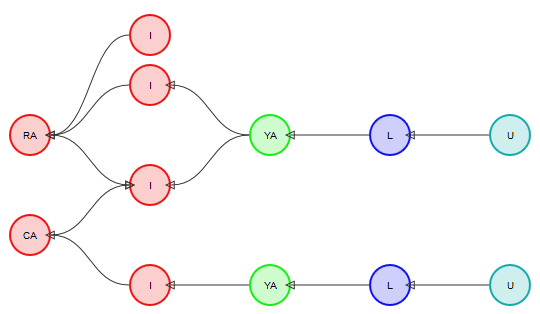
\includegraphics[scale=\scaleProps]{./figures/cmna_proposals/abuse1.png}
\caption{Proposal for representing abusive attacks as solely within the argument$_1$ structure}
\label{figure:cmna:abuse1}
\end{figure}

\begin{figure}
\centering
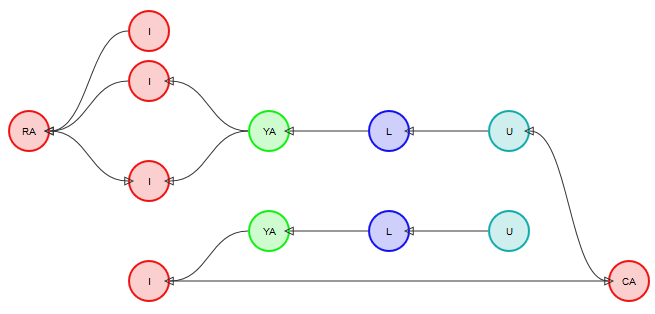
\includegraphics[scale=\scaleProps]{./figures/cmna_proposals/abuse2.png}
\caption{Proposal for representing abusive attacks as connected with the social aspect of the argument$_2$, attacking the author directly}
\label{figure:cmna:abuse2}
\end{figure}

\begin{figure}
\centering
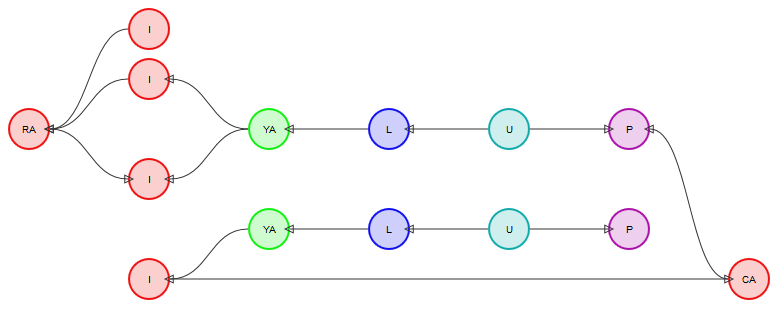
\includegraphics[scale=\scaleProps]{./figures/cmna_proposals/abuse3.png}
\caption{Proposal for representing abusive attacks, extending that shown in Figure \ref{figure:cmna:abuse2} with the addition of Persona nodes}
\label{figure:cmna:abuse3}
\end{figure}

\begin{figure}
\centering
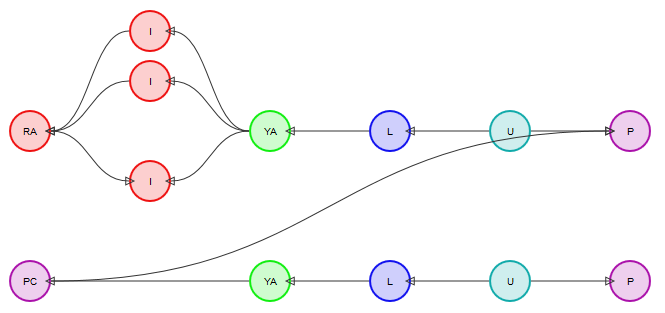
\includegraphics[scale=0.5]{./figures/graphs/aswo-personal-conflict.png}
\caption{Proposal for representing abusive attacks, extending that shown in Figure \ref{figure:cmna:abuse3} with the addition of Personal Conflict node}
\label{figure:cmna:abuse4}
\end{figure}

%%%%%%%%%%%%%%%%%%%%%%%%%%%%%%%%%%%%%%%%%%%%%%%%%%%%%%%%%%%%%%%%%%%%%%%%%%%%%%%%%%%%

\TODO{while out of scope for this body of work, the topic of modelling social systems was also considered} \citep{Blount2014}. These proposals included suggestions for modelling social web specific features, such as the use of reputation systems (e.g. Likes or up/down-votes). Reputation systems make up a key aspect of non-verbal argumentation on the social web, allowing users to show agreement or disagreement to a position, sometimes anonymously, without the need to articulate their own position.

Figure \ref{figure:cmna:likes1} shows one such approach; namely, modelling each vote as a separate Locution, linking to an I-node that either (logically) supports or attacks the voted-on post.

Alternatively, Figure \ref{figure:cmna:likes2} shows an approach which aggregates this information into a single Reputation node. This has the advantage of keeping to social information distinct from the logical graph structure, but the disadvantage of omitting how much each UserAccount contributed to the reputation.

The ASWO does model these  reputation systems; however, for simplicity, they are not modelled as nodes in the graph structure, but are included as literal values attached to the relevant Locution. 


\begin{figure}
\centering
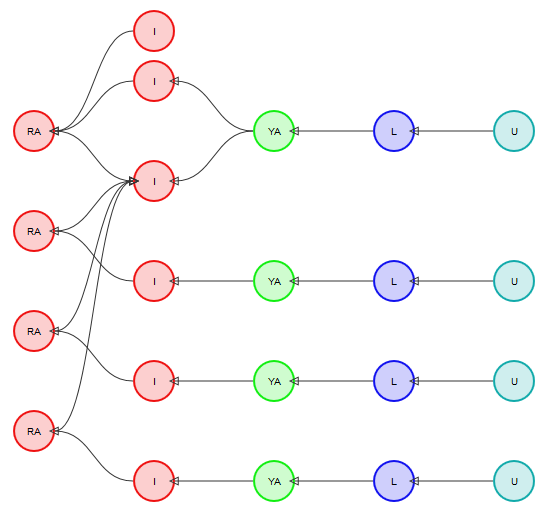
\includegraphics[scale=\scaleProps]{./figures/cmna_proposals/likes2.png}
\caption{Proposal for representing reputation systems by modelling up- and down-votes as individual Locutions}
\label{figure:cmna:likes1}
\end{figure}

\begin{figure}
\centering
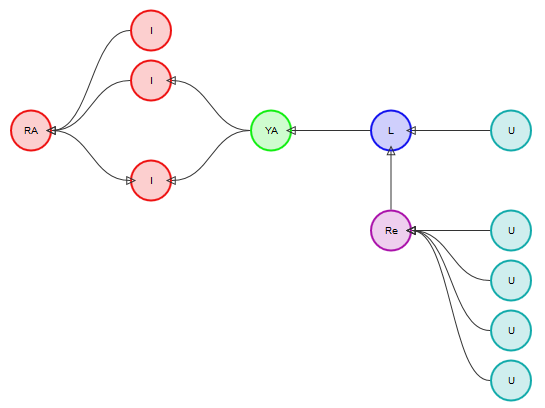
\includegraphics[scale=\scaleProps]{./figures/cmna_proposals/likes1.png}
\caption{Proposal for representing reputation systems with the introduction of a Reputation node}
\label{figure:cmna:likes2}
\end{figure}

In addition, because the SIOC ontology also accounts for replies to and from a post, the use of AIF TA-nodes has also been refined in relation to the social web. They now no longer need to be used whenever an L-node directly responds to another; instead they can be used solely to refer to ``transitions'' in the argument. These transitions are used when a Locution contributes to the argument$_2$ without providing any information, but instead helps move the discussion to the ``next stage'', usually by asking questions or prompting further debate. Note that these transitions don't necessarily move the discussion forwards, but can also be used to take the argument$_2$ around in circles by asking questions in bad faith (or \textit{sealioning}).

%%%%%%%%%%%%%%%%%%%%%%%%%%%%%%%%%%%%%%%%%%%%%%%%%%%%%%%%%%%%%%%%%%%%%%%%%%%%%%%%%%%%%%%%%%%%

\TODO{TIE THESE BITS TOGETHER}

%Based on the observations made in Section \ref{investigation:results} and the proposals discussed in Section \ref{investigation:proposals}, the principal features from the AIF and SIOC ontologies are combined alongside means to model rhetorical tactics in the Argumentation on the Social Web Ontology (ASWO).



%The notion of rhetorical support and attack is modelled by introducing three new types of nodes to the ontology. Firstly, as described in Section \ref{investigation:proposals}, it is not enough to use a UserAccount to represent a person during an argument$_2$. Instead, the Persona node represents a user's character and authority on a given subject, or rather the character and authority they present themselves to have online, and is bound to one or more UserAccounts. Two more node types are introduced to differentiate these types of rhetorical interaction from logical supports or attacks. PersonalConflict (PC-nodes) nodes link from a YA-node to a Persona node to denote this type of personal support and, likewise, PersonalSupport (PS-nodes) nodes follow the same structure to denote support of a person's intentions and character. These are broad, umbrella definitions that serve to catalogue all discovered variants of personal support and attack; they could of course be refined to differentiate between different subcategories of support, such as simple agreement, or self-support (through humour, etc.), or attack such as threats, insults, or provocations. A simple example of this is shown in Figure \ref{figure:graphs:aswo-personal-conflict}, \TODO{MOVED FIGURE} which shows the same argument visualised in Figure \ref{figure:graphs:aifplus} (with the addition of User and Persona nodes) being rhetorically attacked by another user.


\section{Investigation}
\label{aswo:investigation}
The ASWO, and the augmentations made to the AIF and SIOC ontologies, were trialled in an investigation to study the application of logical versus rhetorical techniques in eristic dialogue on the social web. As before, this investigation focused on three different areas of the social web, but used a much larger sample size than previously: in total, two hundred and seventy posts were collected and annotated. These were used to analyse the proportion of rhetorical contributions throughout the argument$_2$, analyse the relation between logical and rhetorical arguments$_1$ used, and compare the features of the annotation structure with the content of each post.


\subsection{Methodology}

\subsubsection{Data Collection}
During the course of this work, the Google YouTube API v2.0 was deprecated before the API v3.0 fully supported the retrieval of explicit replies to comments. Due to the importance of the ability to capture replies, the decision was made to use an alternative medium in this case study. To this end, YouTube was replaced with the social news and networking site Reddit. Reddit has a variety of topic-specific boards or ``subreddits'' that allow users to post to a collaborative pool of information; posts can then be up-voted or down-voted to show interest and/or accuracy.

Obama's official account on Reddit was inactive over the period of the shutdown; however, another user (unaffiliated in any official capacity with Obama) posted a link to Obama's official website (managed by Organizing for Action) to Reddit's politics subreddit\footnote{http://reddit.com/r/politics/1oij25} on 15th October 2013 (the same date as the official posts to Twitter and Facebook). The post reads \textit{``Tea Party Republicans in the House of Representatives have already shut down the government because they couldn't derail Obamacare. Now they're threatening to cause an economic shutdown''}. This thread was used alongside the previously acquired threads from Twitter and Facebook described in Section \ref{investigation:methodology:datacollection}. Each UserAccount involved in the three threads was automatically designated a single Persona, as only one topic was monitored. This could be expanded if the same UserAccount took part in multiple threads on multiple topics, for example.


\begin{table}
\centering
\caption{Metrics of discussions sampled from Twitter, Facebook and Reddit}
\label{table:samples}
\begin{tabular}{| l | c | c | c | c |}
\hline
\textbf{Metric} & \textbf{Twitter} & \textbf{Facebook} & \textbf{Reddit} & \textbf{Total}\\
\hline
Posts & 90 & 90 & 90 & 270\\
\hline
Direct replies & 77 & 0 & 67 & 144\\
\hline
Number of users & 26 & 85 & 43 & 154\\
\hline
Average posts per user & 3.5 & 1.1 & 2.1 & 1.8\\
\hline
Average words per post & 15.83 & 41.36 & 42.34 & 33.18\\
\hline
Average characters per post & 96.51 & 265.27 & 243.31 & 201.70\\
\hline
Time between first and last posts & 0d 6h 53m 40s & 3d 4h 51m 27s & 3d 0h 50m 12s & n/a\\
\hline
Average time between posts & 04m 39s & 51m 49s & 49m 06s & 35m 11s\\
\hline

\end{tabular}
\end{table}

As with the preliminary work, forest fire sampling of the graphs was undertaken to provide a representative sample of the arguments that was feasible to annotate manually. For this investigation a larger sample size of ninety posts was used from within each discussion. Table \ref{table:samples} shows an overview of the sample structures and some key characteristics of each thread.


\subsubsection{Annotation}
\label{aswo:investigation:annotations}
With the changes to the ontologies in use (such as the decision regarding TA-nodes discussed in Section \ref{aswo:augmentations}), and a larger amount of data needing to be annotated, the annotation method itself needed to be properly formalised to solidify reproducibility and minimise subjectiveness. Posts are annotated according to the scheme below.

Each post is considered to contain zero or more separate arguments$_1$. A YA-node is created for each argument$_1$ made in a single post, and links the L-node to each I-node in the argument$_1$. Repeated information does not create a new I-node; instead the YA-node links to the I-node already present. All participants are assumed to have some implicit knowledge about the world in general and the topic at hand. This is to avoid the inclusions of trivial I-nodes that state information such as \textit{``Barack Obama is president of the United States''}, or even \textit{``Barack Obama is a human being''}. Any information explicitly contained in a post that is deemed to be not in this set and relevant to the discussion at hand was included as an I-node. Information that meets one (or more) of the following criteria is not considered relevant:

\begin{itemize}
	\item Off topic: posts that do not relate to the topic being discussed are not considered relevant. Example: \textit{``Ataturk did revolution ! building moderate muslim network is oxymoron which has been destroy secular , democratic, rule of law in Turkey.''}
	\item Conversational: similar to off-topic posts, those that are conversational in nature are not annotated as information-containing. Example: \textit{``I thank you, have a good night!''}
	\item Meta-argumentation: while argumentation about how to argue ``properly'' is an interesting construct in itself, and an important aspect of rhetorical and eristic argumentation, but was out of scope for this particular study. Example: \textit{``Down voting = disagree Upvoting = agree''} \textit{``The rules say explicitly not to do that.....''}
\end{itemize}

A TA-node is created to link two Locutions whenever a transition is present in the argument$_2$ -- a step that contributes to the overall structure without providing any information (new or repeated). This is most often in the form of an interrogative (for example, asking for further information or evidence for claims). Support and attack between different I-nodes is denoted as described above: logical support through the use of RA-nodes, attack through the use of CA-nodes and preference with PA-nodes, while rhetorical support and attack utilises the new PS- and PC-nodes.

Some nodes in the graph may not be complete as a result of the nature of sampling the graph. For example, it may be possible to detect that a user attacks another user's persona, but not exactly which user they are attacking. Table \ref{table:aifnodes} shows an overview of the number of AIF and ASWO nodes added during the annotation process.

\begin{table}
\centering
\caption{Summary of AIF and ASWO nodes found in annotated discussions collected from Twitter, Facebook and Reddit}
\label{table:aifnodes}
\begin{tabular}{| l | c | c | c | c |}
\hline
\textbf{Metric} & \textbf{Twitter} & \textbf{Facebook} & \textbf{Reddit} & \textbf{Total}\\
\hline
L-nodes & 90 & 90 & 90 & 270\\
\hline
TA-nodes & 52 & 9 & 15 & 76\\
\hline
YA-nodes & 58 & 74 & 70 & 202\\
\hline
I-nodes & 56 & 98 & 86 & 240\\
\hline
RA-nodes & 13 & 20 & 24 & 57\\
\hline
CA-nodes & 18 & 1 & 34 & 53\\
\hline
PA-nodes & 4 & 4 & 2 & 10\\
\hline
PS-nodes & 2 & 2 & 3 & 7\\
\hline
PC-nodes & 26 & 6 & 12 & 44\\
\hline
L- to I-node Ratio & 45:28 & 45:49 & 45:43 & 9:8\\
\hline
\end{tabular}
\end{table}


\subsection{Results and Analysis}
\label{aswo:results}

\newcommand{\scaleResults}{0.4}

\subsubsection{Argumentation Tactics Over Time}
Firstly, the way in which the argumentation structure changes and grows over time is presented, in both a logical and rhetorical capacity, by graphing how the number of logical support and attack nodes (i.e. RA- and CA-nodes) and rhetorical support and attack nodes (i.e. PS- and PC-nodes) changes with each post contributed to the argument$_2$. Logical contributions are displayed above the x-axis, and rhetorical contributions below. It must be emphasised that values below the x-axis of each graph should \textit{not} be considered as inherently negative, hostile or anti-social; they simply differentiate between the two types of content.

Figures \ref{figure:rhetorictime:Facebook} and \ref{figure:rhetorictime:reddit} show that use of rhetorical tactics in the Facebook and Reddit case studies rise slowly compared to the use of logical tactics. However, Figure \ref{figure:rhetorictime:Twitter} shows that in the Twitter case study, the rhetorical contributions rise in parallel to the logical contributions.

In both samples from Twitter and Reddit, the distribution of logical supports and attacks also remain approximately equal. Due to the tendency of RA-nodes to be used for logical support within an argument$_1$, and the tendency of CA-nodes to be used between arguments$_1$, this highlights a greater engagement between participants within these debates than the Facebook sample, which has only one CA-node and comparatively much fewer instances of logical or rhetorical contribution overall. In all three examples however, rhetorical conflict far outweighs rhetorical support.

Overall, it appears that there is no sudden shift in tactics from arguing logically to adopting a rhetorical approach -- rhetorical argument forms an underlying and consistent strategy throughout the argument$_2$.

\begin{figure}
\centering
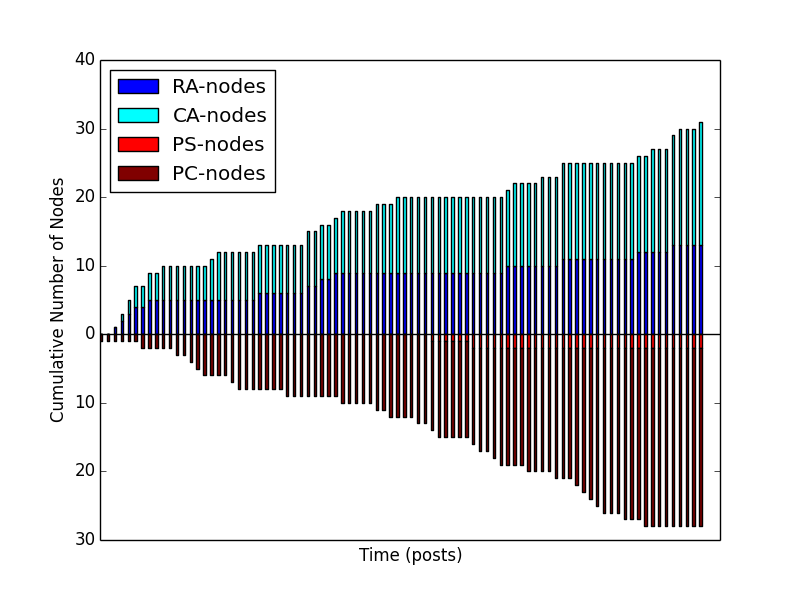
\includegraphics[scale=\scaleResults]{./figures/rhetoric_over_time/twitter.png}
\caption{Cumulative use of logical and rhetoric tactics over time on Twitter}
\label{figure:rhetorictime:Twitter}
\end{figure}

\begin{figure}
\centering
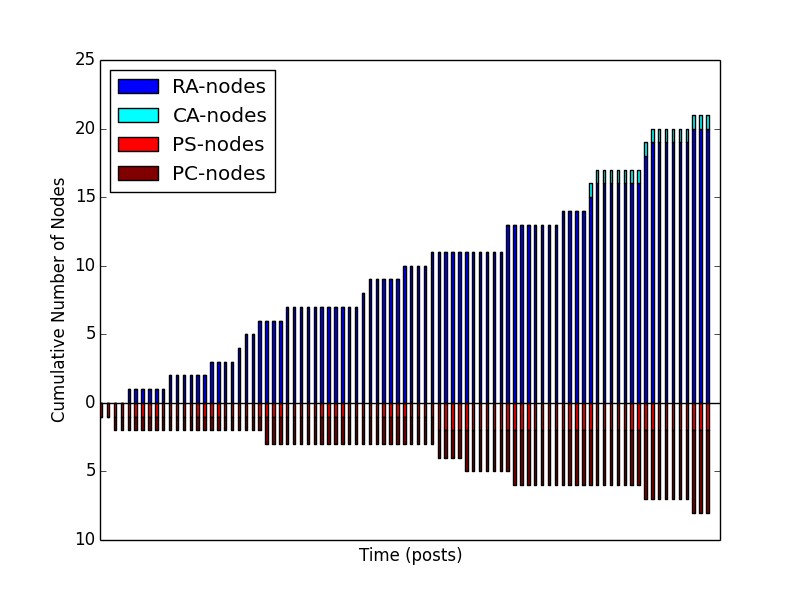
\includegraphics[scale=\scaleResults]{./figures/rhetoric_over_time/facebook.png}
\caption{Cumulative use of logical and rhetoric tactics over time on Facebook}
\label{figure:rhetorictime:Facebook}
\end{figure}

\begin{figure}
\centering
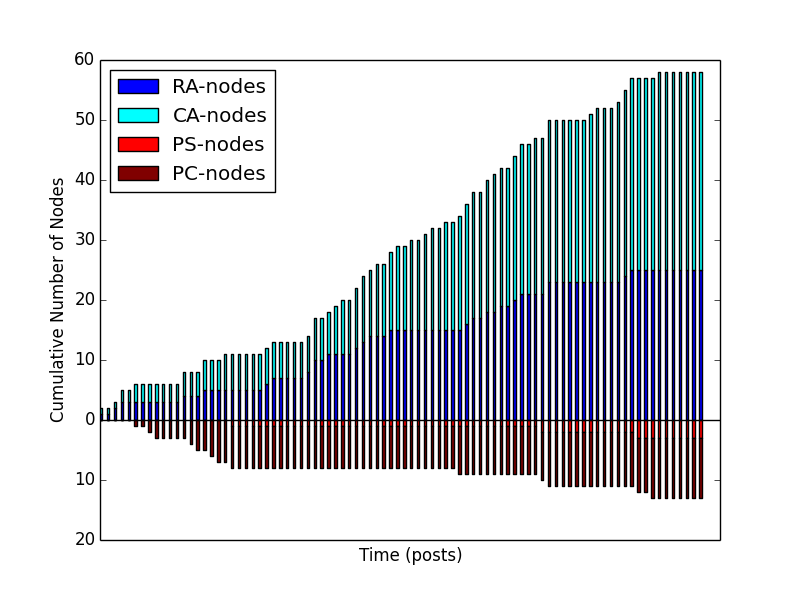
\includegraphics[scale=\scaleResults]{./figures/rhetoric_over_time/reddit.png}
\caption{Cumulative use of logical and rhetoric tactics over time on Reddit}
\label{figure:rhetorictime:reddit}
\end{figure}


\subsubsection{Argumentation Tactics per User}
In addition, proportion of logical versus rhetorical contributions made by each user is examined. These graphs show the contributions made by each user (ordered by total contributions overall). Once more, it must bed stressed that values below the x-axis should not considered anti-social solely due to their rhetorical nature.

Figures \ref{figure:rhetoricuser:Twitter} and \ref{figure:rhetoricuser:reddit} show that users in the Twitter and Reddit samples made more individual contributions to the argumentation structure than those in the Facebook sample, shown in Figure \ref{figure:rhetoricuser:Facebook}. This, along with the data in Table \ref{table:samples}, also supports the suggestion that there is more engagement in these communities than in the Facebook sample.

All samples also display a tendency for rhetorical contributions to be distributed across the scale, with (weak) grouping towards either end. 
This implies that the users most likely to employ rhetorical techniques are those that contribute the most posts to the discussion overall, and those that make no logical contributions at all.

\begin{figure}
\centering
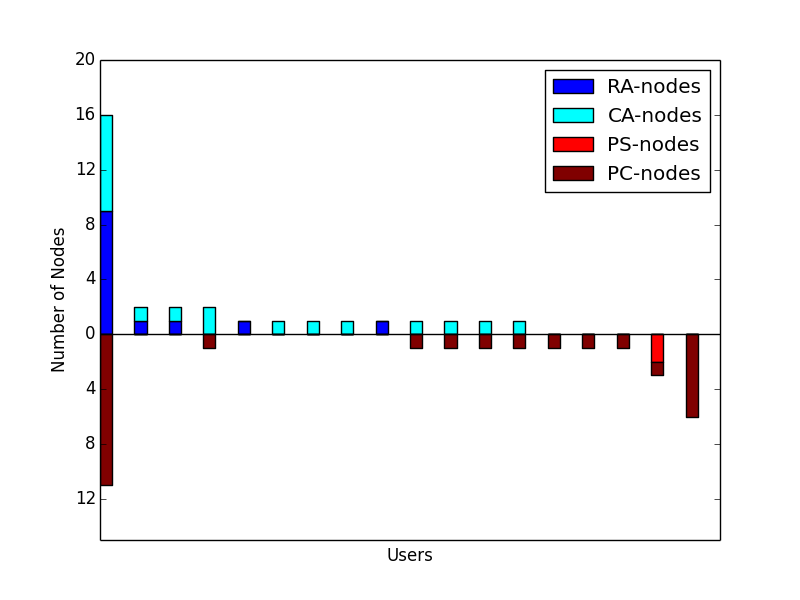
\includegraphics[scale=\scaleResults]{./figures/rhetoric_per_user/twitter.png}
\caption{Logical and rhetorical contributions per sampled user on Twitter}
\label{figure:rhetoricuser:Twitter}
\end{figure}

\begin{figure}
\centering
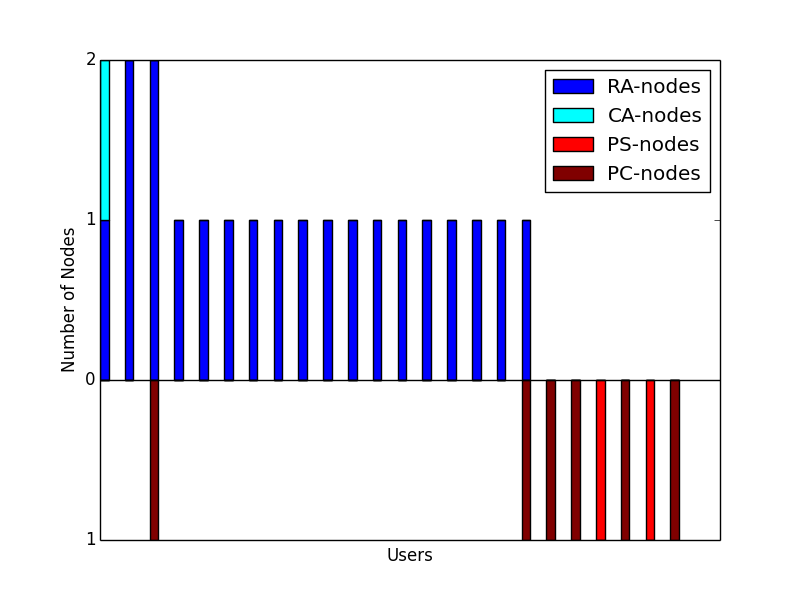
\includegraphics[scale=\scaleResults]{./figures/rhetoric_per_user/facebook.png}
\caption{Logical and rhetorical contributions per sampled user on Facebook}
\label{figure:rhetoricuser:Facebook}
\end{figure}

\begin{figure}
\centering
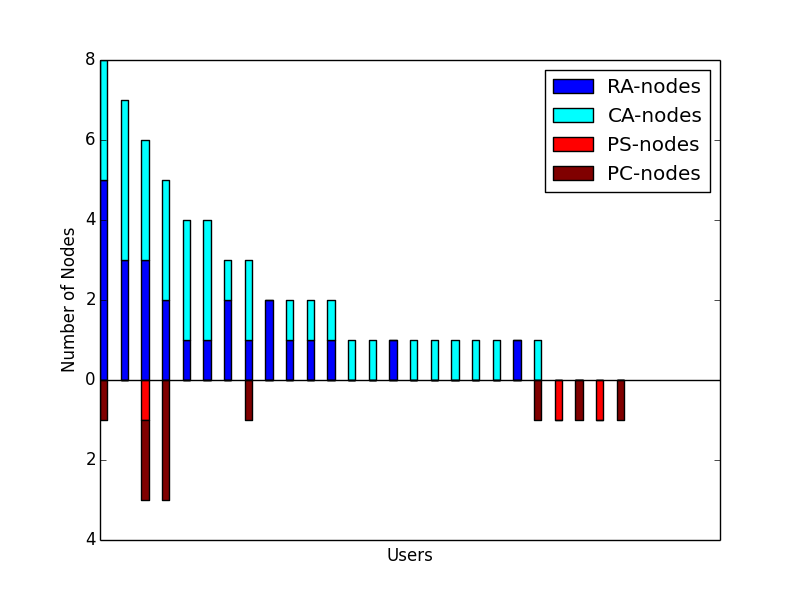
\includegraphics[scale=\scaleResults]{./figures/rhetoric_per_user/reddit.png}
\caption{Logical and rhetorical contributions per sampled user on Reddit}
\label{figure:rhetoricuser:reddit}
\end{figure}

\subsubsection{Correlation Between Argumentation Structure and Post Features}
Correlations were drawn between the structure of the annotated argument graph, including elements such as the number of logical or rhetorical supports or conflicts and replies to and from each post, and features of the post content and structure, such as post length, number of expletives, percentage of spelling errors and again, replies to and from the post. Replies in particular were viewed from both sides: that is, to analyse whether certain types of posts were more likely to be made in reply, or whether posts that were made in reply tended to contribute similar argumentation structures.

Due to the largely discrete (and often binary) nature of the features and values studied (the majority of posts, for example, are likely to contain either zero or one logical or rhetorical conflict) the correlations are relatively weak, as show in Figure \ref{figure:correlations:reddit}. However, some notable correlations are presented in Table \ref{table:correlations}. These show potential early indicators of the structure and value of an argument. For example, as might be expected, longer posts are more likely to have greater contributions to the discussion. Posts that use a large number of expletives are likewise more likely to contain a rhetorical attack. When examining all three case studies together, posts made in reply correlated with posts that were replied to, implying that when one or more users engage in a discussion, they are more likely to be engaged with in return.


\begin{figure}
\centering
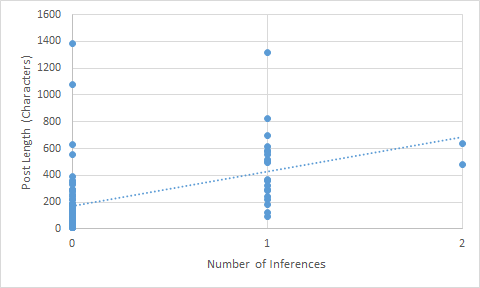
\includegraphics[scale=0.5]{./figures/correlations/reddit.png}
\caption{Post length correlated against number of logical inferences, on Reddit}
\label{figure:correlations:reddit}
\end{figure}



\begin{sidewaystable}
\centering
\caption{Notable correlations between structural argumentation annotations and post features}
\label{table:correlations}
\begin{tabular}{| l | l | l | c | c |}
\hline
\textbf{Case Study} & \textbf{Argumentation Structure} & \textbf{Post Feature} & \textbf{Pearson's Correlation (3 d.p.)} & \textbf{p-value (3 d.p.)}\\
\hline
Twitter & Personal attacks & Number of replies to this post & 0.325 & 0.002\\
\hline
Twitter & Personal attacks & Percentage of spelling errors & 0.301 & 0.004\\
\hline
Twitter & Personal attacks & Expletives & 0.462 & 0.000\\
\hline
Facebook & Original premises & Reputation (``Likes'') & 0.332 & 0.001\\
\hline
Facebook & Original conclusions & Reputation (``Likes'') & 0.329 & 0.002\\
\hline
Facebook & Logical inferences & Reputation (``Likes'') & 0.343 & 0.001\\
\hline
Facebook & Logical conflicts & Emoticons & 0.500 & 0.000\\
\hline
Facebook & Logical conflicts & Expletives & 0.397 & 0.000\\
\hline
Reddit & Original premises & Post length & 0.335 & 0.001\\
\hline
Reddit & Original conclusions & Post length & 0.333 & 0.001\\
\hline
Reddit & Logical inferences & Post length & 0.476 & 0.000\\
\hline
Reddit & Logical conflicts & Number of posts replied to & 0.435 & 0.000\\
\hline
Overall & Number of replies to this post & Number of posts replied to & 0.417 & 0.000\\
\hline
\end{tabular}
\end{sidewaystable}

%\chapter{Use of and Expert Review of Extensions}
%\label{expert}

\newcommand{\imageScale}{0.55}
\newcommand{\nodeScale}{0.95}

%EXPERTS
\newcommand{\simon}{A }
\newcommand{\jodi}{B }
\newcommand{\bob}{C }
\newcommand{\lizzy}{D }
\newcommand{\ash}{E }
\newcommand{\chris}{F }

%In this chapter, the additional proposed nodes are review by \TODO{intro}

\section{Further Proposals}

\TODO{Following on from the investigations in Section} \ref{aswo:investigation}, further

Table \ref{table:newnodes} shows the total set of additional nodes proposed, to further aid modelling rhetorical argument with the ASWO.

Faction and Audience nodes represent groups of Personas; a Faction is any grouping of Personas and can potentially include those outside the Thread. The Audience represents all Personas currently participating in, or observing, the discussion.

Personal Support and Personal Conflict nodes allow a means of representing support and attack that does not rely on logic and instead uses rhetorical force, social pressure or some other form of ``extra-logical'' tactic.

Implication nodes allow analysts to represent a participant implying a relationship between two (or more) nodes, such as Personas. These can be combined with the Personal Support/Conflict nodes to indicate whether the implication is positive or negative.


\begin{table}
\centering
\caption{Description of nodes added to the model}
\label{table:newnodes}
\begin{tabular}{| l | p{6cm} | p{3cm} |}
\hline
\textbf{Name} & \textbf{Description} & \textbf{Node}\\
\hline
P-node & \textbf{Persona} nodes denote a person's social ``character'' that they assume during a discussion & \includegraphics[trim=0 0 0 -5, scale=\nodeScale]{../../speech_acts_js/images/individual nodes/P node.png}\\
\hline
F- and A-nodes & \textbf{Faction} and \textbf{Audience} nodes represent groups of personas & \includegraphics[trim=0 0 0 -5, scale=\nodeScale]{../../speech_acts_js/images/individual nodes/F node.png}\includegraphics[trim=0 0 0 -5, scale=\nodeScale]{../../speech_acts_js/images/individual nodes/A node.png}\\
\hline
PS-, PC-nodes & \textbf{Personal Support} and \textbf{Personal Conflict} nodes support/attack (individual or groups of) \textbf{Personas} and \textbf{Information} in a non-logical way & \includegraphics[trim=0 0 0 -5, scale=\nodeScale]{../../speech_acts_js/images/individual nodes/PS node.png}\includegraphics[trim=0 0 0 -5, scale=\nodeScale]{../../speech_acts_js/images/individual nodes/PC node.png}\\
\hline
Im-node & \textbf{Implication} nodes indicate a relationship that the participants can not be sure exists & \includegraphics[trim=0 0 0 -5, scale=\nodeScale]{../../speech_acts_js/images/individual nodes/Im node.png}\\
\hline
\end{tabular}
\end{table}

\subsection{Examples of Use}
These additions aim to provide atomic ``building-blocks'' that can be reused to model a wide range of social, rhetorical and ``extra-logical'' aspects of argumentation. Here, we show how these nodes can be used by modelling some examples of common logical fallacies.


%\begin{table}[H]
%\centering
%\caption{Potential usage of nodes when modelling fallacious arguments}
%\label{table:fallacynodes}
%\begin{tabular}{l  | l | p{6cm}}
%
%\textbf{Argument} & \textbf{Description} & \textbf{Nodes} \\
%\hline
%\textit{Ad hominem} 1 & & \\
%\textit{Ad hominem} 2 & & \\
%\textit{Ad hominem} 3 & & \\
%
%Appeal to consensus& & \\
%
%Association fallacy & & \\
%
%Appeal to humour 1 & & \\
%Appeal to humour 2 & & \\
%\end{tabular}
%\end{table}


\subsubsection{Syllogism}
A syllogism is an example of reasoning in which two premises are used to draw a conclusion. Figure \ref{figure:syllogism1} shows a syllogism of the form \textit{``All men are mortal. Socrates is a man. Therefore Socrates is mortal''}.

\begin{figure}[H]
\centering
\includegraphics[scale=\imageScale]{../../speech_acts_js/images/annotated/syllogism1.png}
\caption{Example of a syllogism: \textit{``All men are mortal. Socrates is a man. Therefore Socrates is mortal''}}
\label{figure:syllogism1}
\end{figure}


\subsubsection{\textit{Ad hominem}}
\textit{Ad hominem} (``to the man'') arguments attack a person's character, without attacking their argument. However, they can be a viable tactic in rhetorical debate and can introduce both new I-, CA- and PC-nodes to the structure when modelled. Figure \ref{figure:hominem1} shows a reasonable \textit{ad hominem} argument \cite{walton1987}, such as \textit{``You don't have any qualifications in that area, don't make such broad statements.''} Figure \ref{figure:hominem2} shows a more aggressive tactic that disparages someone's argument and them as a person, such as \textit{``They're an idiot, don't listen to them.''} Figure \ref{figure:hominem3} shows an abusive argument that contains no information, instead attacking the person directly and trying to shut them out of the debate, for example \textit{``**** off and die!''} These examples in particular show that a fallacy can take multiple forms and have multiple logical and/or rhetorical contributions to the overall discussion.

%\begin{figure}[H]
%\begin{minipage}{0.5\textwidth}
%\centering
%\includegraphics[scale=.42]{../../speech_acts_js/images/annotated/hominem1.png}
%\end{minipage}%
%\begin{minipage}{0.5\textwidth}
%\centering
%
\includegraphics[scale=.6]{figures/expert/fb_hominem1.png}
%\end{minipage}
%\caption{Example of \textit{ad hominem} \TODO{Dave suggested including a fictional FB post to illustrate the model though I think it might be tough to squeeze them in at an appropriate size}}
%\label{figure:hominem1}
%\end{figure}



\begin{figure}[H]
\centering

\includegraphics[scale=.8]{figures/expert/fb_hominem1.png}
\includegraphics[scale=\imageScale]{../../speech_acts_js/images/annotated/hominem1.png}
\caption{Example of a reasonable \textit{ad hominem} attack}
\label{figure:hominem1}
\end{figure}

\begin{figure}[H]
\centering
\includegraphics[scale=\imageScale]{../../speech_acts_js/images/annotated/hominem2.png}
\caption{Example of an \textit{ad hominem} attacking both persona and argument \TODO{consider adding 'dummy' FB images}}
\label{figure:hominem2}
\end{figure}

\begin{figure}[H]
\centering
\includegraphics[scale=\imageScale]{../../speech_acts_js/images/annotated/hominem3.png}
\caption{Example of an abusive \textit{ad hominem} \TODO{consider adding 'dummy' FB images}}
\label{figure:hominem3}
\end{figure}

\subsubsection{Appeal to Consensus}
The appeal to consensus is the fallacy that because a claim is popular or widely-held, it is true. An example of this can be shown in Figure \ref{figure:consensus1}.

\begin{figure}[H]
\centering
\includegraphics[scale=\imageScale]{../../speech_acts_js/images/annotated/consensus1.png}
\caption{Example of an appeal to consensus \TODO{consider adding 'dummy' FB images}}
\label{figure:consensus1}
\end{figure}

\subsubsection{Association Fallacy}
The association fallacy is the notion that because a person is associated with, or shares the views of, an undesirable group, their claims are wrong. An example of this can be shown in Figure \ref{figure:association1}.

\begin{figure}[H]
\centering
\includegraphics[scale=\imageScale]{../../speech_acts_js/images/annotated/association1.png}
\caption{Example of the association fallacy}
\label{figure:association1}
\end{figure}

\subsubsection{Appeal to Humour}
An appeal to humour is a technique by which a participant in the debate attempts to ingratiate themselves with their audience by making a joke about the situation as shown in Figure \ref{figure:humour1}. This can be coupled with an \textit{ad hominem} attack, when the joke is made at someone else's expense, as shown in Figure \ref{figure:humour2}.
\begin{figure}[H]
\centering
\includegraphics[scale=\imageScale]{../../speech_acts_js/images/annotated/humour1.png}
\caption{Example of an appeal to humour}
\label{figure:humour1}
\end{figure}

\begin{figure}[H]
\centering
\includegraphics[scale=\imageScale]{../../speech_acts_js/images/annotated/humour2.png}
\caption{Example of an \textit{ad hominem} appeal to humour}
\label{figure:humour2}
\end{figure}

\section{Expert Review}
Six experts, from the fields of argumentation systems,  web science, philosophy, and linked data, were chosen to review these proposed additions to the model.

Experts \simon and \jodi have a background in argumentations systems and modelling argumentation, and are familiar with the AIF. Expert \simon is a computer science lecturer whose research is concerned with argumentation-based models of communication and formal reasoning, with interests in AI and behaviour change. Expert \jodi is a post-doctoral researcher with degrees in library and information science, mathematics, and liberal arts whose thesis focused on the problem of analysing, integrating, and reconciling information in online discussions.

Expert \bob is a web-science graduate student, researching the relation between social structures in virtual worlds and the real world, with a focus on practices of gender and power.

Expert \lizzy is a philosophy graduate student, specialising in ethics, moral obligations and with a background in argumentation and formal logic.

Experts \ash and \chris are specialists in the area of open and linked data  working in web and data innovation and development. Expert \ash is an institutional open data specialist and Expert \chris is a senior technical specialist.

Each expert was provided with a document describing the background of this area and an overview of the existing models (reproduced in Appendix \ref{expertsheet}). They were then asked to model three argumentation samples shown in Figure \ref{figure:snippets}, illustrating a variety of different rhetorical structures, by speaking aloud and/or sketching with pen and paper. They were then shown the additions to the model, and asked to model the three argumentation samples again. They were then asked a series of semi-structured question aimed to evaluate their thoughts on how best (and whether) to model social (and anti-social) argumentation, the completeness of the ontology, the clarity of the ontology and the consistency of the ontology.


\begin{figure}

\begin{enumerate}
\small
%Ad hominem
\item 
\textbf{User 1:} \textit{The tech industry is often biased against women}\\
\textbf{User 2:} \textit{@User1 You would say that, you're a woman}\\
\textbf{User 3:} \textit{@User1 **** off and die you ****ing nazi before I come and **** you up}
~\newline
%Syllogism
\item 
\textbf{User 1:} \textit{Guns killed 33,000 people last year, they need to be banned}\\
\textbf{User 2:} \textit{@User1 And a lot of those were minors}\\
\textbf{User 3:} \textit{@User2 According to who?}
~\newline
%Humour
\item 
\textbf{User 1:} \textit{What does Barack Obama call illegal aliens? Undocumented democrats!}\\
\textbf{User 2:} \textit{@User1 You're so stupid you probably went to the library to find Facebook}


\end{enumerate}
\caption{The three argumentation samples the experts were asked to model}
\label{figure:snippets}
\end{figure}


\subsection{Results and Analysis}
\label{results}
Table \ref{table:results} shows an overview of the key points discussed by the experts along the themes of modelling social argumentation, completeness, clarity and consistency (and relevant sub-themes).

\begin{center}
\begin{longtable}{l l | p{6cm}}
\caption{Summary of experts' opinions on key aspects of ASWO}\\
\label{table:results}
\textbf{Theme} & \textbf{Sub-theme} & \textbf{Comments} \\
\hline
\parbox[t]{2cm}{\textbf{Social\\Argumentation}} & \textit{Value} & \textit{``...if we're going to have a realistic model of how people argue, we've got to look at how people really argue rather than how our ``ideal reasoner'' would argue''} --~Expert~\simon \\
& & \textit{``I think modelling social argumentation is very important...I want to say it's useful in trying to help people argue `better'.''} --~Expert~\lizzy\\
\cline{2-3}
& \textit{Challenges} & \textit{``Even in quite a simple back-and-forth argument, there's quite a lot going on...scale is a challenge''} --~Expert~\bob\\
& & \textit{``...enthymemes, humour, there's lots of missing information, there's lots of playing to particular audiences...there are lots of things that are current events or would only make sense to a particular group''} --~Expert~\jodi\\
\cline{2-3}
&\textit{Abuse/Threats} & \textit{``I, personally, tend to ignore all of those because I'm...focusing on the informal proof structures''} --~Expert~\simon\\
&& \textit{``...it's hard to exclude them...if you think about what you're going to do with the model...do you want to retrieve threatening and abusive comments? Well you might want to exclude them from being retrieved, which also makes it relevant to model that''} --~Expert~\jodi\\
\hline
\textbf{Completeness} & \textit{Implicit/Explicit Premises}& \textit{``I think when people model arguments it's pretty common to infer the reading, and what's interesting is that there can be multiple readings. So it wouldn't be wrong to...put in some interpretation, as long as it's clear it's an interpretation and there can be others. ''} --~Expert~\jodi \\
\cline{2-3}
&\textit{Social Meta-Data} & \textit{``One other thing... is other people's opinions of statements. A lot of systems have thumbs up and thumbs down...what you need is, I think, an audience response''} --~Expert~\chris\\
\hline
\textbf{Clarity} & \textit{Generalisation} & \textit{``If anything I think maybe your default conflict is a superclass - everything is a conflict, and one of the subclasses is a...rational argument. But then you've also got personal attack, ad hominem...these are all alternatives to rational argument, but at the default it might be worth allowing modelling of a conflict. Not a conflict as it is in the original model, but as a superclass of interaction.''} --~Expert~\chris\\
\cline{2-3}
 & \textit{Ambiguity} & \TODO{EXPAND OUT THESE TOO} \textit{``If a...''} --~Expert~\lizzy\\
 & & \TODO{Assumptions RE gender of participants etc} --~Expert~\ash\\
\hline
\textbf{Consistency} & \textit{Internal consistency} & \textit{``whenever you try to model anything in a formalised system...if you give two people the same thing...unless it's something really simple, they will always find two different ways of modelling it''} --~Expert~\ash \\
& & \textit{``...rather than having the minimal number of nodes and encouraging people to just misuse them, I would rather say `Here's a definite type of argumentation we want to capture and share...'''} --~Expert~\simon\\
\cline{2-3}
  & \textit{External consistency} & \textit{``Consistent with [the AIF], maybe not, but building on? Definitely''} --~Expert~\bob \\
\end{longtable}
\end{center}


\subsubsection{Social Argumentation}
%Value
Each of the experts agreed that there was value in modelling social argumentation, Expert \chris going so far as to say they believed there was no argument that didn't have social components. Expert \lizzy discussed how understanding the nuances of how people argue socially could lead to ways of helping or encouraging them to argue ``better'', in a more cooperative or polite manner.

%Challenges
The challenges of modelling social argumentation the experts foresaw were mostly a question of scale. In part, the sheer volume of data in a social media discussion can be overwhelming, particularly when considering the speed with which in can grow, but also in terms of the variety of information, which is often contextual, such as references to current events, or cultural ``in-jokes''.

%Abuse/Threats
Experts \simon and \lizzy explained that they would not consider abusive argumentation as a valid when modelling an argumentation structure (as they focused broadly on dialectic arguments and that was the current standard for their domain), although they agreed it was a potentially valuable area to explore. Expert \jodi explain that it depended very much on the purpose of the model --- in some cases it may be important to model threatening and abusive attacks specifically so they can be excluded when presenting the model to users. Expert \ash also noted that excluding this type of argument can lead to confusion if a particular abusive comment changes the course of the argument, or causes the quality of the rest of the discussion to degenerate.

\subsubsection{Completeness}
Experts \simon and \jodi both made explicit mention of the ability to mark certain posts as being in direct response to other participants in the discussion as a useful addition to argumentation frameworks. 

Expert \jodi noted that as many annotations have the potential to be subjective, it would be possible to extend this to include further subjective annotations such as an analyst's confidence in a particular reading of an inference. Expert \bob had similar views and discussed including mappings of a participant's agreement or disagreement with key positions in the dialogue as well.

Expert \chris discussed the potential for an ``activity'' score for each locution, derived from the social meta-data of each post (e.g. number of replies, number of up- or down-votes or number of retweets); this metric could be derived on a per-purpose basis to allow analysts to correctly categorise different platforms for their own needs, and to highlight key areas of the discussion that had solicited or stimulated large amounts of discussion.

Broadly, all experts agreed that to adequately model social argument that it was necessary to include further context about the participants, such as demographic information where available, such as by linking the SIOC UserAccount to a FOAF Agent, or additional information about key events related to the discussion to maintain relevance of the model for future analysis, and to limit the number of assumptions needed to be made by analysts.


\subsubsection{Clarity}
Expert \lizzy was concerned that, when faced as an analyst with a statement that appeared ambiguous (for example, a statement of support that could be interpreted as genuine or sarcastic) they may struggle to accurately and objectively model it, and proposed a means of allowing analysts to mark such relations as existing without committing to associating them with either a support or an attack.

Expert \chris proposed a similar solution, by means of generalising the model to include super-classes of Support and Conflict. ``Personal'' conflict, for example, is perhaps too specific a name for all non-logical conflicts: there are rhetorical attacks that can target institutions or accounts run by software, but also, importantly, positions and information. These Support and Conflict super-classes would encompass Logical Support/Conflict and Rhetorical Support/Conflict and could then be further sub-classed to provide more specific instances of each, where apparent, allowing analysts to defer when unsure.


\subsubsection{Consistency}

The majority of experts felt that these additions to the ASWO were consistent with the nodes used in the AIF. However, Experts \bob and \chris disagreed, pointing to the fact that the ASWO was intentionally inconsistent with the AIF because they were developed for different purposes.

In terms of inter-rater reliability --- whether two analysts attempting to model the same argument would reach the same result --- the experts were much more divided. While they agreed that the objective parts of the model (i.e. the locutions, user account and, in most circumstances, the persona) could be modelled identically (and in most cases, automated), Experts \bob and \jodi felt that both analysts would reach the same conclusion overall with minor deviations, whereas Experts \simon, \lizzy and \ash disagreed, stating there was too much subjective information to model identically. Expert \simon felt that the analyst would naturally perceive the argument through their own lens of cultural and social context and Expert \lizzy noted the different levels of detail an analyst may choose to use, whether focusing only on premises that have been explicitly stated, or including additional implicit information.

How important this is was also a matter of some debate: Experts \jodi and \bob felt that it was likely there would (and should) be one ``correct'' representation of an argument. Experts \lizzy and \chris agreed to an extent, citing their proposals for handling ambiguous content being able to aid annotators in this regard, so that if the model could not be complete, it could be consistent. Expert \simon felt that ideally analysts should reach the same conclusion but in practice, the subjective nature of the task might make this impossible. Expert \ash felt the consistency of annotators would, in practice, be less important and would be a factor of the intended purpose of the model.


\section{Summary}   
\label{conclusions}
\TODO{Tidy, refactor, make leading rather than concluding}

In this chapter, further extensions to the ASWO are introduced, to incorporate other modes of rhetorical persuasion that contrast with logical argument. An expert review was conducted, which highlighted some key strengths of this model, such as the ability to model directed replies, the ability to model the audience and the ability to model instances of irrational and eristic argument that were previously difficult or impossible to achieve with the AIF alone. These results were presented at the conference on Computational Models of Argument \citep{Blount2016rhetorical}.

Because social argumentation can rely heavily on nuanced contextual information (such as the ability to recognise humour, sarcasm or references to current events) it is likely impossible to model it in such a way that it could be automatically reasoned over. However, because the ASWO provides additional information about rhetorical tactics in use, human analysts can explore the resulting structure in greater detail and context. This can also potentially be used to highlight areas of particular interest, or assist in community decision-making environments.

\chapter{Perception of Rhetorical Tactics in Individual Comments}
\label{perception}

This chapter examines how the different types of argument discussed in the previous chapter are perceived by their audience. An experiment was carried out in which participants were shown a number of social media posts, and asked a series of questions (answerable on a Likert scale) about each one. These questions gauged both how they felt about the post (e.g. entertained or offended), and how they would act on it (e.g. replying or reporting).


\section{Methodology}

\subsection{Data Sample}
\label{perception:method:sample}

This work used the ``normal'' threads acquired in Section \ref{case:method:sample}.

Each of these ``normal'' threads was then annotated by topic, using one of the following categories based on an aggregation of the topics provided by the five news distribution sites the social media accounts of which the stories were sourced from:
\textit{Current Events}, stories covering recent or ongoing occurrences;
\textit{Business}, stories involving businesses and/or the economy;
\textit{Politics}, stories relating to politics, politicians, elections, etc.;
\textit{Science \& Technology}, stories relating to science, the environment, new technologies, etc.;
\textit{Entertainment \& Arts}, stories involving cultural events, celebrities, etc.;
\textit{Sports}, stories covering sporting events and participants;
and \textit{Features}, stories that form an opinion piece, or focus on an individual rather than the broader story they are a part of.


\begin{table}
\centering
\caption{Threads by topic}
\label{table:perception:topics}
\begin{tabular}{ l | l | l | l | l}
\textbf{Platform} & \textbf{Current Events} & \textbf{Business} & \textbf{Politics} & \textbf{Science \& Technology} \\
\hline
Facebook & 52 & 18 & 23 & 16 \\
\hline
Twitter & 53 & 3 & 24 & 12\\
\hline
Reddit & 41 & 4 & 2 & 6\\
\end{tabular}
\newline
\newline
\begin{tabular}{ l | l | l | l}
\textbf{Platform} & \textbf{Entertainment \& Arts} & \textbf{Sports} & \textbf{Feature}\\
\hline
Facebook & 20 & 3 & 32 \\
\hline
Twitter & 12 & 3 & 20 \\
\hline
Reddit & 2 & 0 & 0 \\
\end{tabular}
\end{table}
 

\subsection{Classifications}

\TODO{Argument}

\TODO{Social} 
 \citet{kietzmann2011social} describe seven
Identity, Sharing, Presence, Relationships, Reputation, Groups, and Conversations



Table \ref{table:perception:questions} summarises each of these classifications, and provides justification for their inclusion.

\subsection{Participants and Survey}
Participants were invited via a general call on social media; they were provided an information sheet and consent form, and asked to confirm that they were above the age of eighteen. Participants were shown a selection eighteen posts taken from the sample described in Section \ref{perception:method:sample} (three different news-types across three social media platforms). For context, they were also show the initial post in the thread and, if present, any post that was directly replied to by the target. These were presented to participants via a web-survey, a screenshot of which is shown in Figure \ref{figure:perception:survey}.

\begin{figure}
\centering
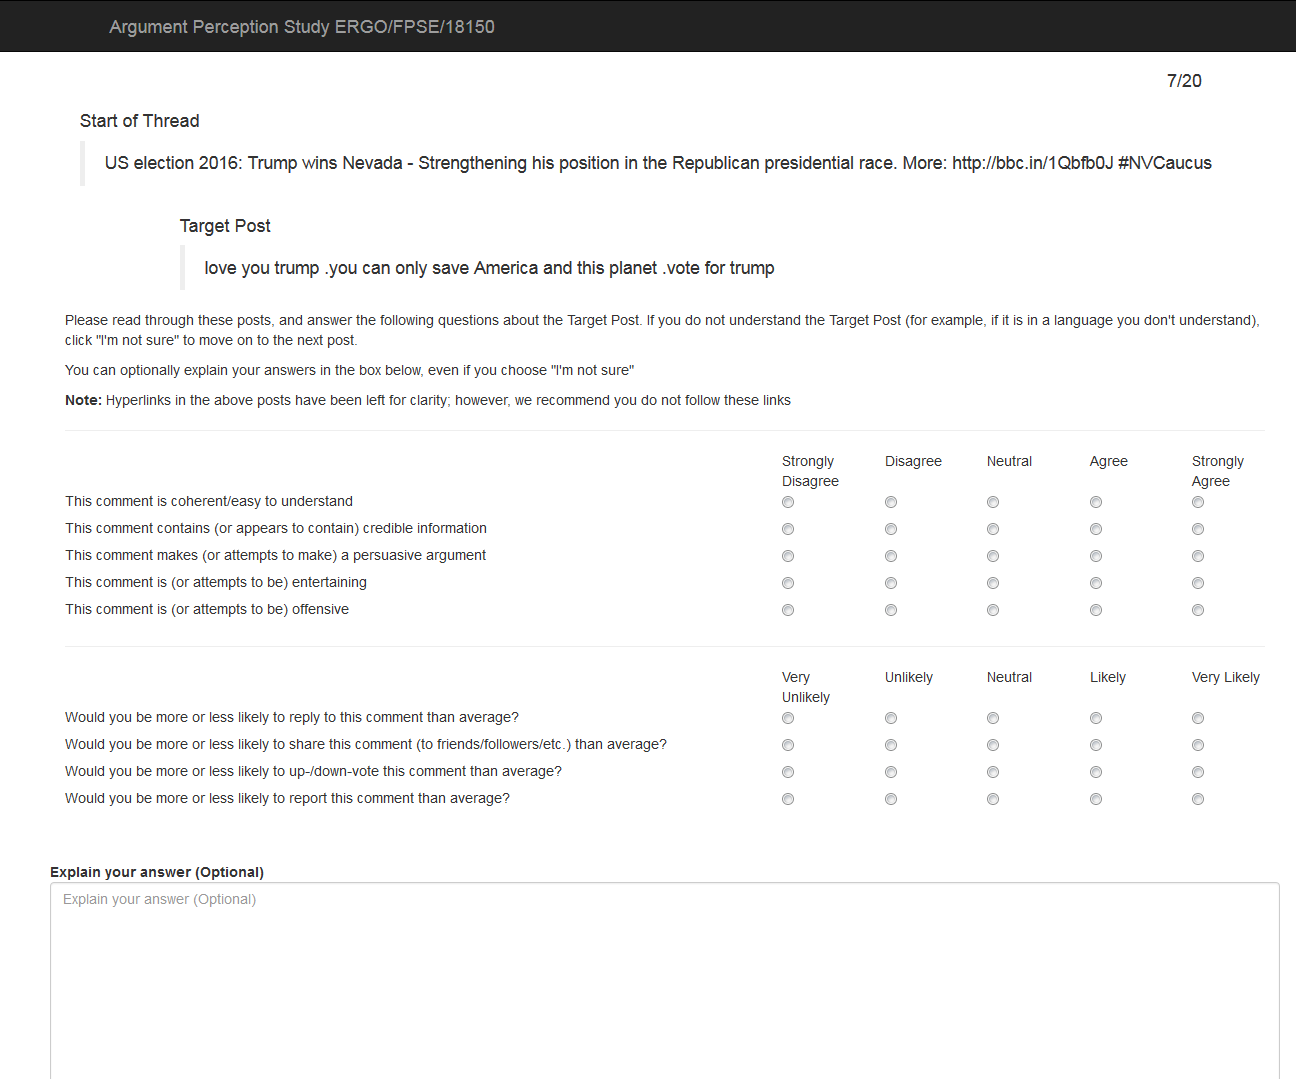
\includegraphics[scale=0.45]{perception/survey1.png}
\caption{The questionnaire as presented to participants}
\label{figure:perception:survey}
\end{figure}

Every participant was also shown, and asked to rate, two additional posts common to all participants to judge the overall inter-rater agreement. These were selected at random from the sampled pool of comments and manually inspected to ensure they were non-empty and comprehensible (e.g., English-language).

\begin{table}
\centering
\caption{Example classifications of argumentation posts}
\label{table:perception:questions}
\begin{tabular}{ l | p{10cm}}
\textbf{Factor} & \textbf{Description} \\
\hline
Coherence & Whether the post is clear and understandable \CITATION  \\
\hline
Credibility & Whether the post contains (purportedly) credible information \CITATION \\
\hline
Persuasiveness & Whether the post attempts to change the readers position \citep{sundar2000}\\
\hline
Entertainment & Whether the post engages or bores the reader \citep{sundar2000}\\
\hline
Offence & \\
\hline
Reply & How likely the reader is to reply\citep{markova2013} \citep{kietzmann2011social}\\
\hline
Share & \citep{markova2013} \citep{kietzmann2011social}\\
\hline
Vote & \citep{markova2013} \citep{kietzmann2011social}\\
\hline
Report &\citep{kietzmann2011social} \\

%Identity & \citep{kietzmann2011social}\\
%\hline
%Sharing & \citep{kietzmann2011social}\\
%\hline
%Presence & \citep{kietzmann2011social}\\
%\hline
%Relationships &\citep{kietzmann2011social} \\
%\hline
%Reputation & \citep{kietzmann2011social}\\
%\hline
%Groups & \citep{kietzmann2011social}\\
%\hline
%Conversations & \citep{kietzmann2011social}\\

\end{tabular}
\end{table}

\section{Data Analysis and Results}

\subsection{Raw Data}

Table \ref{table:perception:breakdown} shows the raw answers that participants gave to the questions overall. Even here, it is relatively easy to see (from questions 6-9) that the majority of people would not be inclined to interact or engage with the comments that were presented here. In addition to these results, 45 people skipped this question

\begin{table}
\centering
\caption{Breakdown of answers given for each question}
\label{table:perception:breakdown}
\begin{tabular}{ p{6cm} | r | r | r | r | r }
\textbf{Question} & \textbf{1} &  \textbf{2} &  \textbf{3} &  \textbf{4} &  \textbf{5}\\
\hline
This comment is coherent/easy to understand  &  48 & 134 & 71 & 374 & 119 \\
\hline
This comment contains (or appears to contain) credible information  &  127 & 230 & 224 & 133 & 32 \\
\hline
This comment makes (or attempts to make) a persuasive argument  &  111 & 172 & 159 & 252 & 52 \\
\hline
This comment is (or attempts to be) entertaining  &  126 & 189 & 151 & 220 & 60 \\
\hline
This comment is (or attempts to be) offensive  &  165 & 208 & 194 & 143 & 36 \\
\hline
Would you be more or less likely to reply to this comment than average?  &  232 & 216 & 183 & 108 & 7 \\
\hline
Would you be more or less likely to share this comment (to friends/followers/etc.) than average?  &  291 & 226 & 176 & 51 & 2 \\
\hline
Would you be more or less likely to up-/down-vote this comment than average?  &  207 & 179 & 195 & 143 & 22 \\
\hline
Would you be more or less likely to report this comment than average?  &  296 & 204 & 211 & 30 & 5 \\
\end{tabular}
\end{table}


Table \ref{table:perception:annotation-breakdown} shows the number of responses given per each different annotation type. Note that as a post may have multiple annotations, there may be (and is likely to be) overlap in the number of responses. From this we can see the distribution of annotations, combined with random selection and the ability of participants to skip questions, resulted in only one response for the \textit{Spam/Advertisement} category, and only two for the \textit{Preference} category. However, posts annotated as containing Logical Attack/Support and Rhetorical Attack/Support, the key element of this perception study, received over one hundred responses each.

\begin{table}
\centering
\caption{Number of responses given per annotation}
\label{table:perception:annotation-breakdown}
\begin{tabular}{ l | r }
\textbf{Annotation} & \pbox{2cm}{\textbf{Number of}\\\textbf{Responses}}\\
\hline
Information & 491\\
Transition & 40\\
Logical Attack & 146\\
Logical Support & 27\\
Rhetorical Attack & 256\\
Rhetorical Support & 181\\
Preference & 2\\
Entity & 307\\
Group & 55\\
Audience & 104\\
Implied Relationship & 7\\
Implied Belief & 30\\
Spam/Advertisement & 1\\	
Unknown & 4\\
None & 10\\
\end{tabular}
\end{table}


\subsection{Inter Rater Reliability}
\label{perception:results:interrater}
To gain an additional insight of how much agreement there was between participants, and if there was particularly strong areas of agreement or disagreement, the first and last statements shown were identical to all participants. These statements were selected at random from the sample pool, but were manually inspected to ensure they were non-empty and comprehensible (e.g., English-language).

The first post, taken from Reddit, reads as follows:
\textit{The FSA is also irrelevant. Nusra and/or ISIS would be be the rulers if Assad collapsed. And also, NO the ``FSA'' is mostly islamists, most of the ``secular rebels'' have switched around and have become part of the SDF which is part of the YPG.} This was annotated as having Information, and a Logical Attack. Table \ref{table:perception:first-raw} shows the raw answers that participants gave to the first question. In addition to these results, 10 people skipped this question. Table \ref{table:perception:first-averages} shows the distribution of these answers: while  there is a relatively large range between the minimum and maximum responses the standard deviation is not excessive. The largest value (1.218) was for the question \textit{This comment makes (or attempts to make) a persuasive argument.} The lowest values were for the questions exploring the perception of entertainment and credibility (0.764 and 0.899 respectively).


\begin{table}
\centering
\caption{Breakdown of answers given for the first question}
\label{table:perception:first-raw}
\begin{tabular}{ p{6cm} | r | r | r | r | r }
\textbf{Question} & \textbf{1} &  \textbf{2} &  \textbf{3} &  \textbf{4} &  \textbf{5}\\
\hline
This comment is coherent/easy to understand  &  6 & 23 & 8 & 16 & 2 \\
\hline
This comment contains (or appears to contain) credible information  &  4 & 18 & 22 & 10 & 1 \\
\hline
This comment makes (or attempts to make) a persuasive argument  &  7 & 11 & 8 & 24 & 5 \\
\hline
This comment is (or attempts to be) entertaining  &  26 & 23 & 4 & 2 & 0 \\
\hline
This comment is (or attempts to be) offensive  &  15 & 21 & 13 & 6 & 0 \\
\hline
Would you be more or less likely to reply to this comment than average?  &  19 & 15 & 11 & 10 & 0 \\
\hline
Would you be more or less likely to share this comment (to friends/followers/etc.) than average?  &  23 & 16 & 12 & 4 & 0 \\
\hline
Would you be more or less likely to up-/down-vote this comment than average?  &  14 & 17 & 15 & 9 & 0 \\
\hline
Would you be more or less likely to report this comment than average?  &  18 & 14 & 21 & 2 & 0 \\
\end{tabular}
\end{table}


\begin{table}
\centering
\caption{Distribution of answers given for the first question}
\label{table:perception:first-averages}
\begin{tabular}{ !p{3cm} | ^r | ^r | ^r | ^r | ^r | ^r | ^r}
\rowstyle{\bfseries} Question & Min. & \pbox{2cm}{Lower\\ Quartile} & Median & \pbox{2cm}{Upper\\ Quartile} & Max. & Mean & $\sigma$\\
\hline
This comment is coherent/easy to understand  &  1.00 & 2.00 & 2.00 & 4.00 & 5.00 & 2.727 & 1.103 \\
\hline
This comment contains (or appears to contain) credible information  &  1.00 & 2.00 & 3.00 & 3.00 & 5.00 & 2.745 & 0.899 \\
\hline
This comment makes (or attempts to make) a persuasive argument  &  1.00 & 2.00 & 4.00 & 4.00 & 5.00 & 3.164 & 1.218 \\
\hline
This comment is (or attempts to be) entertaining  &  1.00 & 1.00 & 2.00 & 2.00 & 4.00 & 1.673 & 0.764 \\
\hline
This comment is (or attempts to be) offensive  &  1.00 & 1.00 & 2.00 & 3.00 & 4.00 & 2.182 & 0.955 \\
\hline
Would you be more or less likely to reply to this comment than average?  &  1.00 & 1.00 & 2.00 & 3.00 & 4.00 & 2.218 & 1.107 \\
\hline
Would you be more or less likely to share this comment (to friends/followers/etc.) than average?  &  1.00 & 1.00 & 2.00 & 3.00 & 4.00 & 1.945 & 0.961 \\
\hline
Would you be more or less likely to up-/down-vote this comment than average?  &  1.00 & 1.50 & 2.00 & 3.00 & 4.00 & 2.345 & 1.031 \\
\hline
Would you be more or less likely to report this comment than average?  &  1.00 & 1.00 & 2.00 & 3.00 & 4.00 & 2.127 & 0.916 \\
\end{tabular}
\end{table}


The last post, taken from Twitter, reads as follows:
\textit{@steve\_walke23 @guardian @lisaocarroll Some beings are inhuman - ISIS atrocities don't bother you? Get off your priggish high horse.} This was annotated as having Information and a Rhetorical Attack, directed against an Entity (in this case likely representing one of @steve\_walke23 or @lisaocarroll, or potentially both).

Table \ref{table:perception:last-raw} shows the raw answers that participants gave to the last question. In addition to these results, 2 people skipped this question. Because fewer people completed every question of the survey, dropping out before the total number of responses to these questions is lower than that of the first post.

Table \ref{table:perception:last-averages} shows the distribution of these answers. The standard deviations are not widely different from the responses to the first group of questions in scale, though they do differ by question. The largest value (1.159), lower than the highest standard deviation of the first group of questions, was shared by the questions examining participants reactions, specifically replying to and voting on.

The lowest values (0.840 and 0.904 respectively), higher than the lowest standard deviations of the first group of questions, were in response to the likelihood participants would reply to this comment (the majority were in agreement that they would not) and judging whether it was considered coherent (on average, participants found it neither excessively clear or unclear).


\begin{table}
\centering
\caption{Breakdown of answers given for the last question}
\label{table:perception:last-raw}
\begin{tabular}{ p{6cm} | r | r | r | r | r }
\textbf{Question} & \textbf{1} &  \textbf{2} &  \textbf{3} &  \textbf{4} &  \textbf{5}\\
\hline
This comment is coherent/easy to understand  &  0 & 6 & 3 & 19 & 3 \\
\hline
This comment contains (or appears to contain) credible information  &  4 & 10 & 12 & 4 & 1 \\
\hline
This comment makes (or attempts to make) a persuasive argument  &  2 & 3 & 6 & 18 & 2 \\
\hline
This comment is (or attempts to be) entertaining  &  4 & 14 & 8 & 5 & 0 \\
\hline
This comment is (or attempts to be) offensive  &  1 & 4 & 3 & 17 & 6 \\
\hline
Would you be more or less likely to reply to this comment than average?  &  8 & 7 & 7 & 9 & 0 \\
\hline
Would you be more or less likely to share this comment (to friends/followers/etc.) than average?  &  11 & 12 & 7 & 1 & 0 \\
\hline
Would you be more or less likely to up-/down-vote this comment than average?  &  8 & 9 & 7 & 6 & 1 \\
\hline
Would you be more or less likely to report this comment than average?  &  10 & 8 & 12 & 1 & 0 \\
\end{tabular}
\end{table}


\begin{table}
\centering
\caption{Distribution of answers given for the last question}
\label{table:perception:last-averages}
\begin{tabular}{ !p{3cm} | ^r | ^r | ^r | ^r | ^r | ^r | ^r}
\rowstyle{\bfseries} Question & Min. & \pbox{2cm}{Lower\\ Quartile} & Median & \pbox{2cm}{Upper\\ Quartile} & Max. & Mean & $\sigma$\\
\hline
This comment is coherent/easy to understand  &  2.00 & 3.00 & 4.00 & 4.00 & 5.00 & 3.613 & 0.904 \\
\hline
This comment contains (or appears to contain) credible information  &  1.00 & 2.00 & 3.00 & 3.00 & 5.00 & 2.613 & 0.973 \\
\hline
This comment makes (or attempts to make) a persuasive argument  &  1.00 & 3.00 & 4.00 & 4.00 & 5.00 & 3.484 & 0.979 \\
\hline
This comment is (or attempts to be) entertaining  &  1.00 & 2.00 & 2.00 & 3.00 & 4.00 & 2.452 & 0.910 \\
\hline
This comment is (or attempts to be) offensive  &  1.00 & 3.50 & 4.00 & 4.00 & 5.00 & 3.742 & 1.015 \\
\hline
Would you be more or less likely to reply to this comment than average?  &  1.00 & 1.50 & 3.00 & 4.00 & 4.00 & 2.548 & 1.159 \\
\hline
Would you be more or less likely to share this comment (to friends/followers/etc.) than average?  &  1.00 & 1.00 & 2.00 & 2.50 & 4.00 & 1.935 & 0.840 \\
\hline
Would you be more or less likely to up-/down-vote this comment than average?  &  1.00 & 1.50 & 2.00 & 3.00 & 5.00 & 2.452 & 1.159 \\
\hline
Would you be more or less likely to report this comment than average?  &  1.00 & 1.00 & 2.00 & 3.00 & 4.00 & 2.129 & 0.907 \\
\end{tabular}
\end{table}

\subsection{Question Breakdown}
\label{perception:results:breakdown}
In this section, a summary of the responses to each of the questions is presented, compared against the annotations present on the post. Table \ref{table:perception:mean-summary-classification} shows the mean Likert values for each question, and Table \ref{table:perception:deviation-summary-classification} shows the standard deviation from this mean. The full results are presented in Appendix \ref{appendix:perception-data} (Tables \ref{table:perception:coherent-classification}-\ref{table:perception:report-classification}). Note that as a post may have multiple annotations, there may be (and is likely to be) overlap in the number of responses.  

\TODO{TALK ABOUT WHY THESE NUMBERS ARE INTERESTING}
Discounting posts that received few responses (e.g. Preferences and Spam/Advertisement) it can be seen that there is a reasonable level of variation between participants ($\sigma>1$). However, for when asked how likely they would be to share
%(Table \ref{table:perception:share-classification})
or report,
%(Table \ref{table:perception:report-classification}),
participants were in closer agreement, in both cases stating they would be less likely to engage than average.

%Table \ref{table:perception:coherent-classification} shows the breakdown of agreement to the statement \textit{This comment is coherent/easy to understand}.

\begin{table}
\centering
\caption{Mean rating for each question, compared with annotations present}
\label{table:perception:mean-summary-classification}
\begin{tabular}{ !l | ^r ^r ^r ^r ^r ^r ^r ^r ^r}
& \multicolumn{9}{c}{\textbf{Mean Response to Question}} \\
\rowstyle{\bfseries} Annotation & Q1 & Q2 & Q3 & Q4 & Q5 & Q6 & Q7 & Q8 & Q9\\
\hline
Information             & 3.475 & 2.756 & 3.196 & 2.678 & 2.556 & 2.322 & 2.045 & 2.497 & 1.986 \\
Transition              & 3.750 & 2.600 & 2.825 & 2.650 & 2.575 & 2.525 & 2.025 & 2.450 & 1.900 \\
Logical Attack          & 3.308 & 2.966 & 3.329 & 2.158 & 2.301 & 2.390 & 2.048 & 2.548 & 1.973 \\
Logical Support         & 3.778 & 2.815 & 3.000 & 2.704 & 2.963 & 2.185 & 2.000 & 2.333 & 2.074 \\
Rhetorical Attack       & 3.527 & 2.418 & 2.965 & 3.094 & 3.164 & 2.199 & 1.863 & 2.426 & 2.094 \\
Rhetorical Support      & 3.580 & 2.547 & 2.685 & 3.420 & 2.309 & 2.271 & 2.122 & 2.530 & 1.972 \\
Preference              & 3.000 & 2.000 & 3.500 & 3.500 & 3.000 & 2.000 & 2.000 & 2.000 & 2.500 \\
Entity                  & 3.511 & 2.427 & 2.886 & 3.280 & 2.853 & 2.238 & 2.010 & 2.463 & 2.042 \\
Group                   & 3.527 & 2.873 & 3.273 & 2.873 & 2.873 & 2.200 & 1.927 & 2.618 & 2.182 \\
Audience                & 3.510 & 2.356 & 2.596 & 3.740 & 2.817 & 2.385 & 2.269 & 2.625 & 2.154 \\
Implied Relationship    & 3.429 & 2.143 & 3.143 & 2.857 & 3.429 & 1.571 & 1.571 & 2.429 & 2.714 \\
Implied Belief          & 3.800 & 2.333 & 3.000 & 2.967 & 3.333 & 2.067 & 1.800 & 2.667 & 2.333 \\
Spam/Advertisement      & 1.000 & 1.000 & 1.000 & 1.000 & 1.000 & 1.000 & 1.000 & 4.000 & 5.000 \\
Unknown                 & 2.750 & 2.000 & 2.000 & 2.250 & 1.500 & 1.500 & 1.500 & 2.250 & 1.500 \\
None                    & 3.100 & 1.700 & 1.600 & 3.000 & 1.700 & 1.700 & 1.200 & 1.700 & 1.600 \\
\end{tabular}
\end{table}



\begin{table}
\centering
\caption{Standard deviation from mean for each question, compared with annotations present}
\label{table:perception:deviation-summary-classification}
\begin{tabular}{ !l | ^r ^r ^r ^r ^r ^r ^r ^r ^r }
& \multicolumn{9}{c}{\textbf{Standard Deviation from Mean Response to Question}} \\
\rowstyle{\bfseries} Annotation & Q1 & Q2 & Q3 & Q4 & Q5 & Q6 & Q7 & Q8 & Q9\\
\hline
Information             & 1.131 & 1.069 & 1.137 & 1.178 & 1.152 & 1.088 & 0.950 & 1.162 & 0.932 \\
Transition              & 1.112 & 1.091 & 1.138 & 1.216 & 1.181 & 1.072 & 0.961 & 1.094 & 0.970 \\
Logical Attack          & 1.191 & 1.036 & 1.211 & 1.090 & 1.088 & 1.161 & 1.016 & 1.188 & 0.958 \\
Logical Support         & 0.737 & 1.020 & 1.089 & 0.974 & 1.261 & 0.862 & 0.903 & 0.903 & 0.979 \\
Rhetorical Attack       & 1.107 & 1.043 & 1.160 & 1.221 & 1.141 & 1.062 & 0.906 & 1.190 & 0.996 \\
Rhetorical Support      & 1.113 & 1.084 & 1.192 & 1.142 & 1.104 & 1.061 & 1.033 & 1.149 & 0.960 \\
Preference              & 1.000 & 0.000 & 0.500 & 0.500 & 0.000 & 0.000 & 0.000 & 0.000 & 0.500 \\
Entity                  & 1.122 & 1.032 & 1.177 & 1.181 & 1.206 & 1.052 & 0.970 & 1.167 & 0.999 \\
Group                   & 1.126 & 1.113 & 1.242 & 1.207 & 1.192 & 1.051 & 0.912 & 1.168 & 1.011 \\
Audience                & 1.109 & 1.028 & 1.043 & 0.971 & 1.116 & 1.059 & 1.058 & 1.145 & 0.948 \\
Implied Relationship    & 0.728 & 0.639 & 1.245 & 0.833 & 1.178 & 0.728 & 0.728 & 1.498 & 1.385 \\
Implied Belief          & 1.108 & 1.135 & 1.155 & 1.303 & 1.135 & 0.892 & 0.792 & 1.164 & 1.043 \\
Spam/Advertisement      & 0.000 & 0.000 & 0.000 & 0.000 & 0.000 & 0.000 & 0.000 & 0.000 & 0.000 \\
Unknown                 & 1.479 & 1.000 & 1.000 & 0.829 & 0.866 & 0.866 & 0.866 & 1.299 & 0.866 \\
None                    & 1.578 & 1.100 & 0.917 & 1.483 & 0.900 & 1.100 & 0.600 & 1.100 & 1.020 \\
\end{tabular}
\end{table}

\subsection{Logic/Rhetoric}
\label{perception:results:logic-rhetoric}
This section, and Tables \ref{table:perception:coherent-logic-rhetoric}-\ref{table:perception:report-logic-rhetoric}, examine how perception of arguments differ purely with regards to logical and rhetorical annotations (both attack and support). All other classifications are ignored for these tables.

Perhaps surprisingly, the majority of responses are very close, differing by a mean of \textless0.5. The largest difference was in response to whether the post was considered entertaining, with people considering rhetoric to be more entertaining by a margin of 0.967 (which was below the standard deviation). To determine if these observations can  be explained by the spread of different types of argument \textit{within} the umbrellas of logic and rhetoric, such as support and attack, these are considered in the next section.


\begin{table}
\centering
\caption{Average agreement with the statement \textit{This comment is coherent/easy to understand}, grouped by Logic and Rhetoric}
\label{table:perception:coherent-logic-rhetoric}
\begin{tabular}{ !l | ^r ^r ^r ^r ^r ^r ^r}
\rowstyle{\bfseries} Annotation & Min. & \pbox{2cm}{Lower\\ Quartile} & Median & \pbox{2cm}{Upper\\ Quartile} & Max. & Mean & $\sigma$\\
\hline
Logic  &  1.00 & 2.00 & 4.00 & 4.00 & 5.00 & 3.374 & 1.150 \\
Rhetoric  &  1.00 & 3.00 & 4.00 & 4.00 & 5.00 & 3.572 & 1.107 \\
\end{tabular}
\end{table}


\begin{table}
\centering
\caption{Average agreement with the statement \textit{This comment contains (or appears to contain) credible information}, grouped by Logic and Rhetoric}
\label{table:perception:credible-logic-rhetoric}
\begin{tabular}{ !l | ^r ^r ^r ^r ^r ^r ^r}
\rowstyle{\bfseries} Annotation & Min. & \pbox{2cm}{Lower\\ Quartile} & Median & \pbox{2cm}{Upper\\ Quartile} & Max. & Mean & $\sigma$\\
\hline
Logic  &  1.00 & 2.00 & 3.00 & 4.00 & 5.00 & 2.959 & 1.028 \\
Rhetoric  &  1.00 & 2.00 & 2.00 & 3.00 & 5.00 & 2.455 & 1.060 \\
\end{tabular}
\end{table}


\begin{table}
\centering
\caption{Average agreement with the statement \textit{This comment makes (or attempts to make) a persuasive argument}, grouped by Logic and Rhetoric}
\label{table:perception:persuasive-logic-rhetoric}
\begin{tabular}{ !l | ^r ^r ^r ^r ^r ^r ^r}
\rowstyle{\bfseries} Annotation & Min. & \pbox{2cm}{Lower\\ Quartile} & Median & \pbox{2cm}{Upper\\ Quartile} & Max. & Mean & $\sigma$\\
\hline
Logic  &  1.00 & 2.00 & 4.00 & 4.00 & 5.00 & 3.298 & 1.189 \\
Rhetoric  &  1.00 & 2.00 & 3.00 & 4.00 & 5.00 & 2.848 & 1.191 \\
\end{tabular}
\end{table}


\begin{table}
\centering
\caption{Average agreement with the statement \textit{This comment is (or attempts to be) entertaining}, grouped by Logic and Rhetoric}
\label{table:perception:entertaining-logic-rhetoric}
\begin{tabular}{ !l | ^r ^r ^r ^r ^r ^r ^r}
\rowstyle{\bfseries} Annotation & Min. & \pbox{2cm}{Lower\\ Quartile} & Median & \pbox{2cm}{Upper\\ Quartile} & Max. & Mean & $\sigma$\\
\hline
Logic  &  1.00 & 1.00 & 2.00 & 3.00 & 5.00 & 2.228 & 1.087 \\
Rhetoric  &  1.00 & 2.00 & 3.00 & 4.00 & 5.00 & 3.195 & 1.211 \\
\end{tabular}
\end{table}


\begin{table}
\centering
\caption{Average agreement with the statement \textit{This comment is (or attempts to be) offensive}, grouped by Logic and Rhetoric}
\label{table:perception:offensive-logic-rhetoric}
\begin{tabular}{ !l | ^r ^r ^r ^r ^r ^r ^r}
\rowstyle{\bfseries} Annotation & Min. & \pbox{2cm}{Lower\\ Quartile} & Median & \pbox{2cm}{Upper\\ Quartile} & Max. & Mean & $\sigma$\\
\hline
Logic  &  1.00 & 1.50 & 2.00 & 3.00 & 5.00 & 2.404 & 1.137 \\
Rhetoric  &  1.00 & 2.00 & 3.00 & 4.00 & 5.00 & 2.830 & 1.215 \\
\end{tabular}
\end{table}


\begin{table}
\centering
\caption{Average response to the question \textit{Would you be more or less likely to reply to this comment than average?}, grouped by Logic and Rhetoric}
\label{table:perception:reply-logic-rhetoric}
\begin{tabular}{ !l | ^r ^r ^r ^r ^r ^r ^r}
\rowstyle{\bfseries} Annotation & Min. & \pbox{2cm}{Lower\\ Quartile} & Median & \pbox{2cm}{Upper\\ Quartile} & Max. & Mean & $\sigma$\\
\hline
Logic  &  1.00 & 1.00 & 2.00 & 3.00 & 5.00 & 2.368 & 1.123 \\
Rhetoric  &  1.00 & 1.00 & 2.00 & 3.00 & 5.00 & 2.200 & 1.054 \\
\end{tabular}
\end{table}


\begin{table}
\centering
\caption{Average response to the question \textit{Would you be more or less likely to share this comment (to friends/followers/etc.) than average?}, grouped by Logic and Rhetoric}
\label{table:perception:share-logic-rhetoric}
\begin{tabular}{ !l | ^r ^r ^r ^r ^r ^r ^r}
\rowstyle{\bfseries} Annotation & Min. & \pbox{2cm}{Lower\\ Quartile} & Median & \pbox{2cm}{Upper\\ Quartile} & Max. & Mean & $\sigma$\\
\hline
Logic  &  1.00 & 1.00 & 2.00 & 3.00 & 5.00 & 2.047 & 1.002 \\
Rhetoric  &  1.00 & 1.00 & 2.00 & 3.00 & 4.00 & 1.938 & 0.953 \\
\end{tabular}
\end{table}


\begin{table}
\centering
\caption{Average response to the question \textit{Would you be more or less likely to up-/down-vote this comment than average?}, grouped by Logic and Rhetoric}
\label{table:perception:vote-logic-rhetoric}
\begin{tabular}{ !l | ^r ^r ^r ^r ^r ^r ^r}
\rowstyle{\bfseries} Annotation & Min. & \pbox{2cm}{Lower\\ Quartile} & Median & \pbox{2cm}{Upper\\ Quartile} & Max. & Mean & $\sigma$\\
\hline
Logic  &  1.00 & 1.50 & 3.00 & 3.00 & 5.00 & 2.520 & 1.151 \\
Rhetoric  &  1.00 & 1.00 & 2.00 & 3.00 & 5.00 & 2.473 & 1.185 \\
\end{tabular}
\end{table}


\begin{table}
\centering
\caption{Average response to the question \textit{Would you be more or less likely to report this comment than average?}, grouped by Logic and Rhetoric}
\label{table:perception:report-logic-rhetoric}
\begin{tabular}{ !l | ^r ^r ^r ^r ^r ^r ^r}
\rowstyle{\bfseries} Annotation & Min. & \pbox{2cm}{Lower\\ Quartile} & Median & \pbox{2cm}{Upper\\ Quartile} & Max. & Mean & $\sigma$\\
\hline
Logic  &  1.00 & 1.00 & 2.00 & 3.00 & 5.00 & 1.994 & 0.964 \\
Rhetoric  &  1.00 & 1.00 & 2.00 & 3.00 & 5.00 & 2.045 & 0.986 \\
\end{tabular}
\end{table}

\subsection{Support/Attack}
\label{perception:results:support-attack}
As noted in Section \ref{perception:results:logic-rhetoric}, there are different purposes for using logic or rhetoric that may account of the homogeneous results observed. By further breaking the answers down into different types of logic and rhetoric (specifically, support and attack) Tables \ref{table:perception:coherent-support-attack}-\ref{table:perception:report-support-attack} examine how perception varies further.

%Perhaps surprisingly, the majority of responses are very close, differing by a mean of <0.5. The largest difference was in response to whether the post was considered entertaining, with 0.967 (which was below the standard deviation). These observations can likely be explained by the spread of different types of argument \textit{within} the umbrellas of logic and rhetoric, such as support and attack which are considered in the next section.


Once more, the majority of responses are relatively close, differing by a mean of \textless0.5. Again the exception to this was whether posts was considered entertaining and, to a lesser degree, offensive. 

Supportive posts were considered to be more entertaining (by an average of 0.716) when using rhetorical devices rather than logical devices. They were also considered to be more offensive (by an average of 0.654) when using logical devices rather than rhetorical devices.

Attacking posts showed an even greater difference in opinion, with rhetorical posts being considered both more entertaining and more offensive (by a margin of 0.936 and 0.863 respectively) than logical posts.


\begin{table}
\centering
\caption{Average agreement with the statement \textit{This comment is coherent/easy to understand}, grouped by support and attack}
\label{table:perception:coherent-support-attack}
\begin{tabular}{ !l | ^r ^r ^r ^r ^r ^r ^r}
\rowstyle{\bfseries} Annotation & Min. & \pbox{2cm}{Lower\\ Quartile} & Median & \pbox{2cm}{Upper\\ Quartile} & Max. & Mean & $\sigma$\\
\hline
\rowstyle{\bfseries} Support  &  1.00 & 3.00 & 4.00 & 4.00 & 5.00 & 3.603 & 1.082 \\
Logical Support  &  2.00 & 3.50 & 4.00 & 4.00 & 5.00 & 3.778 & 0.737 \\
Rhetorical Support  &  1.00 & 3.00 & 4.00 & 4.00 & 5.00 & 3.580 & 1.113 \\
\rowstyle{\bfseries} Attack  &  1.00 & 2.00 & 4.00 & 4.00 & 5.00 & 3.445 & 1.140 \\
Logical Attack  &  1.00 & 2.00 & 4.00 & 4.00 & 5.00 & 3.308 & 1.191 \\
Rhetorical Attack  &  1.00 & 3.00 & 4.00 & 4.00 & 5.00 & 3.527 & 1.107 \\
\end{tabular}
\end{table}


\begin{table}
\centering
\caption{Average agreement with the statement \textit{This comment contains (or appears to contain) credible information}, grouped by support and attack}
\label{table:perception:credible-support-attack}
\begin{tabular}{ !l | ^r ^r ^r ^r ^r ^r ^r}
\rowstyle{\bfseries} Annotation & Min. & \pbox{2cm}{Lower\\ Quartile} & Median & \pbox{2cm}{Upper\\ Quartile} & Max. & Mean & $\sigma$\\
\hline
\rowstyle{\bfseries} Support  &  1.00 & 2.00 & 2.50 & 3.00 & 5.00 & 2.564 & 1.081 \\
Logical Support  &  1.00 & 2.00 & 3.00 & 3.50 & 5.00 & 2.815 & 1.020 \\
Rhetorical Support  &  1.00 & 2.00 & 3.00 & 3.00 & 5.00 & 2.547 & 1.084 \\
\rowstyle{\bfseries} Attack  &  1.00 & 2.00 & 3.00 & 3.00 & 5.00 & 2.613 & 1.074 \\
Logical Attack  &  1.00 & 2.00 & 3.00 & 4.00 & 5.00 & 2.966 & 1.036 \\
Rhetorical Attack  &  1.00 & 2.00 & 2.00 & 3.00 & 5.00 & 2.418 & 1.043 \\
\end{tabular}
\end{table}


\begin{table}
\centering
\caption{Average agreement with the statement \textit{This comment makes (or attempts to make) a persuasive argument}, grouped by support and attack}
\label{table:perception:persuasive-support-attack}
\begin{tabular}{ !l | ^r ^r ^r ^r ^r ^r ^r}
\rowstyle{\bfseries} Annotation & Min. & \pbox{2cm}{Lower\\ Quartile} & Median & \pbox{2cm}{Upper\\ Quartile} & Max. & Mean & $\sigma$\\
\hline
\rowstyle{\bfseries} Support  &  1.00 & 2.00 & 3.00 & 4.00 & 5.00 & 2.701 & 1.181 \\
Logical Support  &  1.00 & 2.00 & 3.00 & 4.00 & 4.00 & 3.000 & 1.089 \\
Rhetorical Support  &  1.00 & 2.00 & 3.00 & 4.00 & 5.00 & 2.685 & 1.192 \\
\rowstyle{\bfseries} Attack  &  1.00 & 2.00 & 3.00 & 4.00 & 5.00 & 3.082 & 1.201 \\
Logical Attack  &  1.00 & 2.00 & 4.00 & 4.00 & 5.00 & 3.329 & 1.211 \\
Rhetorical Attack  &  1.00 & 2.00 & 3.00 & 4.00 & 5.00 & 2.965 & 1.160 \\
\end{tabular}
\end{table}


\begin{table}
\centering
\caption{Average agreement with the statement \textit{This comment is (or attempts to be) entertaining}, grouped by support and attack}
\label{table:perception:entertaining-support-attack}
\begin{tabular}{ !l | ^r ^r ^r ^r ^r ^r ^r}
\rowstyle{\bfseries} Annotation & Min. & \pbox{2cm}{Lower\\ Quartile} & Median & \pbox{2cm}{Upper\\ Quartile} & Max. & Mean & $\sigma$\\
\hline
\rowstyle{\bfseries} Support  &  1.00 & 3.00 & 4.00 & 4.00 & 5.00 & 3.328 & 1.148 \\
Logical Support  &  1.00 & 2.00 & 3.00 & 3.00 & 5.00 & 2.704 & 0.974 \\
Rhetorical Support  &  1.00 & 3.00 & 4.00 & 4.00 & 5.00 & 3.420 & 1.142 \\
\rowstyle{\bfseries} Attack  &  1.00 & 2.00 & 3.00 & 4.00 & 5.00 & 2.753 & 1.257 \\
Logical Attack  &  1.00 & 1.00 & 2.00 & 3.00 & 5.00 & 2.158 & 1.090 \\
Rhetorical Attack  &  1.00 & 2.00 & 3.00 & 4.00 & 5.00 & 3.094 & 1.221 \\
\end{tabular}
\end{table}


\begin{table}
\centering
\caption{Average agreement with the statement \textit{This comment is (or attempts to be) offensive}, grouped by support and attack}
\label{table:perception:offensive-support-attack}
\begin{tabular}{ !l | ^r ^r ^r ^r ^r ^r ^r}
\rowstyle{\bfseries} Annotation & Min. & \pbox{2cm}{Lower\\ Quartile} & Median & \pbox{2cm}{Upper\\ Quartile} & Max. & Mean & $\sigma$\\
\hline
\rowstyle{\bfseries} Support  &  1.00 & 1.00 & 2.00 & 3.00 & 5.00 & 2.363 & 1.127 \\
Logical Support  &  1.00 & 2.00 & 3.00 & 4.00 & 5.00 & 2.963 & 1.261 \\
Rhetorical Support  &  1.00 & 1.00 & 2.00 & 3.00 & 5.00 & 2.309 & 1.104 \\
\rowstyle{\bfseries} Attack  &  1.00 & 2.00 & 3.00 & 4.00 & 5.00 & 2.839 & 1.189 \\
Logical Attack  &  1.00 & 1.00 & 2.00 & 3.00 & 5.00 & 2.301 & 1.088 \\
Rhetorical Attack  &  1.00 & 2.00 & 3.00 & 4.00 & 5.00 & 3.164 & 1.141 \\
\end{tabular}
\end{table}


\begin{table}
\centering
\caption{Average response to the question \textit{Would you be more or less likely to reply to this comment than average?}, grouped by support and attack}
\label{table:perception:reply-support-attack}
\begin{tabular}{ !l | ^r ^r ^r ^r ^r ^r ^r}
\rowstyle{\bfseries} Annotation & Min. & \pbox{2cm}{Lower\\ Quartile} & Median & \pbox{2cm}{Upper\\ Quartile} & Max. & Mean & $\sigma$\\
\hline
\rowstyle{\bfseries} Support  &  1.00 & 1.00 & 2.00 & 3.00 & 5.00 & 2.265 & 1.038 \\
Logical Support  &  1.00 & 1.50 & 2.00 & 3.00 & 4.00 & 2.185 & 0.862 \\
Rhetorical Support  &  1.00 & 1.00 & 2.00 & 3.00 & 5.00 & 2.271 & 1.061 \\
\rowstyle{\bfseries} Attack  &  1.00 & 1.00 & 2.00 & 3.00 & 5.00 & 2.295 & 1.106 \\
Logical Attack  &  1.00 & 1.00 & 2.00 & 3.00 & 5.00 & 2.390 & 1.161 \\
Rhetorical Attack  &  1.00 & 1.00 & 2.00 & 3.00 & 5.00 & 2.199 & 1.062 \\
\end{tabular}
\end{table}


\begin{table}
\centering
\caption{Average response to the question \textit{Would you be more or less likely to share this comment (to friends/followers/etc.) than average?}, grouped by support and attack}
\label{table:perception:share-support-attack}
\begin{tabular}{ !l | ^r ^r ^r ^r ^r ^r ^r}
\rowstyle{\bfseries} Annotation & Min. & \pbox{2cm}{Lower\\ Quartile} & Median & \pbox{2cm}{Upper\\ Quartile} & Max. & Mean & $\sigma$\\
\hline
\rowstyle{\bfseries} Support  &  1.00 & 1.00 & 2.00 & 3.00 & 4.00 & 2.108 & 1.019 \\
Logical Support  &  1.00 & 1.00 & 2.00 & 3.00 & 4.00 & 2.000 & 0.903 \\
Rhetorical Support  &  1.00 & 1.00 & 2.00 & 3.00 & 4.00 & 2.122 & 1.033 \\
\rowstyle{\bfseries} Attack  &  1.00 & 1.00 & 2.00 & 3.00 & 5.00 & 1.953 & 0.956 \\
Logical Attack  &  1.00 & 1.00 & 2.00 & 3.00 & 5.00 & 2.048 & 1.016 \\
Rhetorical Attack  &  1.00 & 1.00 & 2.00 & 2.00 & 4.00 & 1.863 & 0.906 \\
\end{tabular}
\end{table}


\begin{table}
\centering
\caption{Average response to the question \textit{Would you be more or less likely to up-/down-vote this comment than average?}, grouped by support and attack}
\label{table:perception:vote-support-attack}
\begin{tabular}{ !l | ^r ^r ^r ^r ^r ^r ^r}
\rowstyle{\bfseries} Annotation & Min. & \pbox{2cm}{Lower\\ Quartile} & Median & \pbox{2cm}{Upper\\ Quartile} & Max. & Mean & $\sigma$\\
\hline
\rowstyle{\bfseries} Support  &  1.00 & 2.00 & 3.00 & 3.00 & 5.00 & 2.505 & 1.122 \\
Logical Support  &  1.00 & 2.00 & 2.00 & 3.00 & 4.00 & 2.333 & 0.903 \\
Rhetorical Support  &  1.00 & 2.00 & 3.00 & 3.00 & 5.00 & 2.530 & 1.149 \\
\rowstyle{\bfseries} Attack  &  1.00 & 1.00 & 2.00 & 3.00 & 5.00 & 2.479 & 1.175 \\
Logical Attack  &  1.00 & 1.00 & 3.00 & 4.00 & 5.00 & 2.548 & 1.188 \\
Rhetorical Attack  &  1.00 & 1.00 & 2.00 & 3.00 & 5.00 & 2.426 & 1.190 \\
\end{tabular}
\end{table}


\begin{table}
\centering
\caption{Average response to the question \textit{Would you be more or less likely to report this comment than average?}, grouped by support and attack}
\label{table:perception:report-support-attack}
\begin{tabular}{ !l | ^r ^r ^r ^r ^r ^r ^r}
\rowstyle{\bfseries} Annotation & Min. & \pbox{2cm}{Lower\\ Quartile} & Median & \pbox{2cm}{Upper\\ Quartile} & Max. & Mean & $\sigma$\\
\hline
\rowstyle{\bfseries} Support  &  1.00 & 1.00 & 2.00 & 3.00 & 5.00 & 1.975 & 0.957 \\
Logical Support  &  1.00 & 1.00 & 2.00 & 3.00 & 4.00 & 2.074 & 0.979 \\
Rhetorical Support  &  1.00 & 1.00 & 2.00 & 3.00 & 5.00 & 1.972 & 0.960 \\
\rowstyle{\bfseries} Attack  &  1.00 & 1.00 & 2.00 & 3.00 & 5.00 & 2.050 & 0.968 \\
Logical Attack  &  1.00 & 1.00 & 2.00 & 3.00 & 5.00 & 1.973 & 0.958 \\
Rhetorical Attack  &  1.00 & 1.00 & 2.00 & 3.00 & 5.00 & 2.094 & 0.996 \\
\end{tabular}
\end{table}

\subsection{Rationale}
\label{perception:results:rationale}
Participants were provided a free-text area to optionally provide the reasons behind the choices they made. Below is a selection of these responses, their accompanying posts, and a discussion of what this means relating to the overall results noted above.




\TODO{Coherent}


Participants noted some of the features that they felt made an argument seem credible: either using direct quotes, or deliberately stating that the view was an opinion.

\textit{``Seems like a credible argument by using a quote''}

\textit{``...they're talking about their own opinions so it is credible.''}

Interestingly, participants often remarked that posts they had answered \textit{attempting} to persuade, did not strike them as particularly persuasive:




\TODO{entertaining}

Unsurprisingly, participants broadly felt that posts with foul language were offensive (although this was subjective), or those that directly insulted a person (whether within the discussion, or the topic of it), and often branded them as deliberate trolls. However, in certain cases, participants felt this would actually spur them to reply and engage with the discussion.

\textit{It's mildly offensive, but mostly it's just a bad, totally pointless joke, best ignored.}

\textit{It's just swearing so not particularly offensive.}

\textit{``I don't engage with racial hatred discussions. There's no rational discussion.''}

\textit{``The answer is trolling. Don't feed trolls.''}

\textit{``Essentially a trolling answer.''}

\textit{People are facing execution, and someone posts a dumb joke? It would be pretty funny in other contexts, but this is gross. I'd be more likely to reply just to call them out for being an ass.}


Participants had different opinions on how emotional language would change their behaviour; one explained that they were more likely to reply to posts that didn't seem emotionally charged, whereas another felt the opposite.

\textit{``I liked the non-emotional tone. So I would comfortable replying. But because my emotions are not engaged, I am less inclined to share''}

\textit{``It is emotionally engaging so prompts replying. It is entertaining that promots} [sic] \textit{sharing.''} 

There was also a relatively consistent consensus that participants were more likely to find a post persuasive, or vote for content, if they personally agreed with:

\textit{``The bias is: I am much more likely to share/upvote a comment if I agree with its contents.''}

\textit{``...Since I agree with the comment, I'm likely for me to vote up...''}

\textit{``...I tend to upvote content that I agree with and share content I disagree with...''}

As might be expected, participants were more likely to report posts that did not appear to be entering the discussion in good faith, whether through insults or derailing the topic.

\textit{``Baiting.''}

\textit{``...the respondent isn't likely to engage in polite debate.''}

\textit{``Appears to be spam''}


Several of the rationales given justified the low engagement scores given (an average of \textless2 for replying, sharing, etc.) These were broadly in two camps: either due a general disinterest in the subject at hand, or due to the post being unclear or not credible.

\textit{``I don't really reply to comments on social media, but do often read them. Hence my 'neutral' more/less likely answers to these questions.''}

\textit{``I just don't care about politics.''}

\textit{``...I'm not particularly interested so I wouldn't be likely to engage them.''}

\textit{``Not clear the respondent's intention''}

\textit{``Don't know how credible this information is, so I wouldn't interact with this comment''}

Conversely, some participants explained their enthusiasm for interacting with certain comments particularly \textit{because} of this.

\textit{``This is a stupid argument, so I'm likely to interact with it.''}

Others pointed out they were more likely to interact with posts that appeared to have a central conclusion that could actually be argued for or against.

\textit{``The comment has facts that can be argued for or against - so I'd be more likely to interact with this comment.''}

\textit{``I don't know a lot about the event but I would be more likely to respond to this as there is a clear point that could be discussed...''}

\subsection{Comparison to Existing Work}
\TODO{Comparisons}

\section{Summary}
Due to a relatively high standard deviation, the results point to a degree of variation between participants answers. This is likely due to a combination of factors, in particular the individual variance of the posts (in terms of tone, implicit meaning, context, etc.) and the natural subjectivity with which people view argument. Despite this, the results suggest that rhetorical techniques are considered very similar to logical techniques in terms of general perception of argumentation, and are often considered to be more entertaining. This supports the hypothesis that rhetorical argumentation has its place in discussions on the social web, and is valuable to model.

%\chapter{Perception of Rhetorical Tactics in Discussion Threads}
\label{perception2}

%% ----------------------------------------------------------------
%% Conclusions.tex
%% ---------------------------------------------------------------- 


\chapter{Conclusions and Future Work}
\label{conclusionsfuture}

\section{Findings}
\label{conclusionsfuture:findings}
The work described in this report covers an examination of the capability of current argumentation models, in particular the application of a combination of the AIF and SIOC ontologies to the social web, and the extension of these models to capture social and rhetorical information. Case-studies were carried out on three different areas of the social web to determine the strengths and weaknesses of modelling social, eristic argument on the web. This preliminary work indicated that existing techniques for modelling argumentation were insufficient to capture the structure and dynamic of argumentation taking place on the social web, which led to the publication of a paper in \textit{the 14th workshop on Computational Models of Natural Argument}, detailing these omissions and proposing a set of augmentations to capture additional socio-rhetorical tactics \citep{Blount2014}. These extensions were implemented and trialled as part of an investigation re-examining the previous case-studies to determine the prevalence of rhetorical tactics in argumentation within areas of the social web and look for correlations that can be drawn between the use of these tactics and the machine-readable characteristic of the post such as length or readability. The results of this will published in the upcoming \textit{ACM Conference on Hypertext and Social Media} \citep{Blount2015}. These investigations reveal the following findings.

Firstly, and most importantly, rhetorical tactics are shown to be present throughout the argumentation in the case studies, even when only accounting for a small subset of rhetorical argumentation. Clearly, failure to accurately model these social argumentation strategies is detrimental to the goal of studying how discussions evolve on the social web. Secondly, in the three use cases, rhetorical tactics are most often used by either those contributing the most to the discussion overall, or by those who do not contribute logically at all. Whether this effect is related to a participant's engagement is unknown. However, this raises the possibility that there is a tipping-point in a dialectic logical debate where participants feel the need to expand their use of tactics; alternatively, these users simply interleave both types of tactics throughout their arguments$_2$. Finally, while the features of the argumentation structure above are challenging to detect automatically and expensive to manually annotate, the markers present in the social media sphere are relatively trivial to detect, and some correlations between the two can be observed.

%\subsection{Limitations}
The primary limitation of this work is the necessity to manually annotate all the data. This is time consuming and subjective, but as yet there is no way to circumvent this process and automatically extract premises and conclusions. A further constraint is that only English-language sites are examined. There are, of course, many other social media services that cater to audiences of different languages, such as \textit{Renren}\footnote{http://renren.com/} for China or \textit{VKontakte}\footnote{http://vk.com/} for eastern Europe. However, this separation is mitigated by the fact that different languages (and different cultures) have their own rhetorical structures and argumentation schemes \citep[p.~21]{Van2004}. As a result, attempting to analyse multiple sites with different primary languages concurrently would distort any patterns that might emerge in the argument structure of the users.

\subsection{Hypothesis and Research Questions}
\label{conclusionsfuture:future:hypothesis}
Revisiting the hypothesis initially proposed in Section \ref{introduction:hypothesis}:

\textit{``A model of eristic argumentation on the social web should include both logical and rhetorical tactics, as the inclusion of rhetorical techniques affects the way in which users perceive and engage with the argument''}

This was resolved into three distinct research questions:
\begin{enumerate}
\item \textit{Are current frameworks and tools sufficient to model eristic argumentation on the social web?}
\item \textit{Is modelling eristic argumentation valuable?}
\item \textit{Which rhetorical techniques should be included in a model of eristic argumentation on the social web?}
\item \textit{Do rhetorical techniques affect the way in which users perceive and engage with the argument?}

\end{enumerate}

Based on the proceeding body of work, these questions can now effectively be answered as follows:

\TODO{The first question}

\TODO{The second question}

\TODO{The third question}

\TODO{The final question}

%Question one is perhaps the most important question, as it determines the overall value of this work. It is best answered in several different parts; firstly, by literature review, secondly, by an analysis of techniques commonly used in social argumentation, and thirdly by interviewing experts in fields that commonly use, model or support argumentation.
%
%Question two focuses on determining whether it is currently possible to accurately describe argumentation occurring on the social web in terms of pre-existing models. Through a review of existing literature and a short exploratory work in the area, the current state-of-the-art will be examined and their suitability at modelling personal, social, and rhetorical argument will be evaluated.
%
%Question three revolves around the most appropriate means of representing rhetorical tactics. Clearly, providing an exhaustive list of all possible examples of rhetorical tactics would not only be infeasible, but also unlikely to provide any value to modellers or analysts. Therefore, to determine the most effective means of representing these tactics, modellers and analysts should be consulted to determine the most effective method, with an emphasis on the purpose of use.
%
%Question four focuses on the practical implications of this work; that is to say, whether the users of social media perceive arguments using different logical and rhetorical tactics in different ways, and whether this drives them to engage in different manners. This makes it important to define the terms perception and engagement. Perception can be thought of as the way in which users understand the tone, persuasiveness, entertainment value or information content of an argument \citep{sundar2000}. Engagement, conversely, can be thought of as how likely they are to, and in which they respond to or participate in the argument itself. This not limited to replying to a post: users of social media can engage in multiple ways, including replying, sharing or voting \citep{markova2013}.


\section{Proposals for Future Work}

Based on the investigations that have been carried out in this thesis, and the findings summarised in Section \ref{conclusionsfuture:findings}, these are the particular avenues of future work that could be approached, using this extended model of social argumentation at their core.

\subsection{Further refinement/review of ASWO}
\TODO{Further refinement/review of ASWO}
The development of the ASWO has been, and should continue to be, an evolving process. Further refinement and expert review will
This includes returning to the proposals laid out in Section \ref{investigation:proposals}, which discusses other aspects of social argumentation that require additional efforts to model, including the notion of social meta-data such as up-/down-votes.

\subsection{Social Media Features}
\TODO{Perception of reputation systems (likes, retweets etc.)}

\subsection{Participant Presentation}
\TODO{How participants present themselves - avatars, bios, (followers?) (``The Twitter Egg with 7 followers vs., say, Stephen Fry) etc. Does this have an impact?}

\subsection{Further refinement/review of ASWO}
\TODO{Multi-comment/overall thread perceptions?}

\subsection{Crowdsourcing}
\TODO{Workshop experiment; categorisation/classification of argument tactics; instructed non-experts vs trained non-experts (vs experts)}




Firstly, as is the focus of many researchers in this field, attention can be given to the use of artificial intelligence and argumentation, whether by reasoning over a model of argument in an attempt to determine the most valid argument and subsequent course of action \citep{caminada2007} or by using the model to influence the techniques and strategies of intelligent agents involved in dialogue games \citep{Reed2008}. However, the fact that the eristic features of the model are unlikely to be practical (or appropriate) for the use of reasoning, or governing inter-agent negotiations is likely what has caused them to be currently excluded from the majority of formal models. Disregarding this, the weakness of this approach is that the model cannot, at this stage, be automatically constructed, but must be created through a time and labour intensive process of manual annotation. Therefore, using the model as a basis of reasoning over argumentation in general is ultimately flawed. Any gains that were achieved in this area would be rendered moot by the cost of creating a model for every argumentation to be reasoned over, and rendered impractical on a web-scale.

With this in mind, the second avenue would be to generate this model from the arguments$_2$ themselves, by means of natural language processing \citep{palau2009}, the use of social machines \citep{hendler2010} or some combination thereof. This would go some way towards solving a large outstanding issue in the field \citep[p.~31-32]{Schneider2013}. While working towards a means of automatically generating the model has potential, it is likely that the social and eristic nature of the arguments to be modelled is the very thing that hinders this approach. Web-based culture and language is made up of many disparate groups, and continues to rapidly and constantly evolve, which renders current natural language processing impractical in the short term and ineffective in the long term, without the use of domain-specific normalisation techniques that are expensive or inaccurate \citep{han2011, eisenstein2013}. While the findings in Section \ref{aswo:results} point towards a means of broadly classifying a post as containing different types of logical or rhetorical elements, with reasonable probability, the overall structure may be difficult to model automatically. Clearly, at this stage, human input cannot be wholly eliminated. However, with the use of crowd-sourcing or social machines, the large effort cost of annotating arguments$_2$ could be distributed across participants to a manageable level.

Finally, emphasis could be placed on the social aspect of argument. Because argumentation is a social process conducted by people, it is important to recognise the fact that individuals may perceive the same argument$_2$ in many different ways due to cultural beliefs \citep{suzuki2011}, pre-existing cognitive biases \citep{Arceneaux2012}, as well as features surrounding the content of the argument$_1$ such as avatars \citep{lee2014}. The advantage of this approach is that it uses the existing model as a platform for experimentally evaluating how the use and prevalence of different argumentation tactics affect users' perceptions of an argument$_2$, and the way in which they engage with the thread (and one another) as a result. By using the model as a tool for analysing individual case studies, the requirements for creating and annotating the necessary argumentation structures are greatly constrained, while allowing the findings to be used in further work in the research area. This contribution to the field can then be used to assist further work in a number of other areas, such as another metric for use with adaptive recommendation techniques to match people based on preferred argumentation strategies \citep{guy2010}, or the development of argumentation frameworks that integrate with the social web \citep{torroni2010}.


%\begin{table}
%\centering
%\caption{Example classifications of argumentation posts}
%\label{table:annotations}
%\begin{tabular}{| l | p{10cm} | l}
%%%%%%%%%%%%%%%%%%%%%%%%%%%%% LOGIC %%%%%%%%%%%%%%%%%%%%%%%%%%%%
%\cline{1-2}
%\textbf{Information} & This post contains (purportedly) factual information & \rdelim\}{17}{3mm}[\parbox{3cm}{Logical\\ tactics}]\\
%\cline{1-2}
%(example) & \textit{``Here's a List of 313+ Employers Who Have Cut Hours Because of Obamacare...''} \\
%\cline{1-2}
%\textbf{Logical Support} & This post supports another post or point of view by providing supplementary evidence, attempting to invoke the authority of the author, or another logical tactic \\
%\cline{1-2}
%(example) & \textit{lol, right ? They don't get that if everyone has access to affordable healthcare then everyone pays their fair share} \\
%\cline{1-2}
%\textbf{Logical Attack} & This post attacks another post or point of view by providing contrary evidence, attempting to undermine the authority of the author, or another logical tactic \\
%\cline{1-2}
%(example) & \textit{``No one ``negotiates'' over laws that have already passed''} \textit{``Really? Then why isn't the Volstead Act still the law of the land?''} \\
%\cline{1-2}
%\textbf{Transitionary} & This post attempts to move the argument forwards by asking questions or prompting further debate \\
%\cline{1-2}
%(example) & \textit{``If you know the numbers, then please tell me how many Dems lost their seat the last two rounds?''} \\
%\cline{1-2}
%%%%%%%%%%%%%%%%%%%%%%%%%%%%% RHETORIC %%%%%%%%%%%%%%%%%%%%%%%%%%%% 
%\textbf{Personal Support} & This post expresses support for another user (rather than their argument) & \rdelim\}{15}{3mm}[\parbox{3cm}{Rhetorical\\ tactics}]\\
%\cline{1-2}
%(example) & \textit{``I commend you for admitting that debt \& deficits are important...If only more [people] felt the way you do''} \\
%\cline{1-2}
%\textbf{Personal Attack} & This post attacks, abuses or threatens another user (rather than their argument) \\
%\cline{1-2}
%(example) & \textit{Fuck off cunt} 
%\\
%\cline{1-2}
%\textbf{Calls to action} & Posts that advocate a particular course of action \\
%\cline{1-2}
%(example) & \textit{``Kill them now, impeach them now. The american people dont need masters''} \\
%\cline{1-2}
%\textbf{Meta-argumentation} & Posts that argue about the argument itself -- whether commenting on the rules of the medium or proposing a way participants should argue ``properly''\\
%\cline{1-2}
%(example) & \textit{``Down voting = disagree Upvoting = agree''} \textit{``The rules say explicitly not to do that.....''} \\
%\cline{1-2}
%%%%%%%%%%%%%%%%%%%%%%%%%%%%% OTHER %%%%%%%%%%%%%%%%%%%%%%%%%%%% 
%\textbf{Conversational} & Posts that do not put forward, support or attack a particular view, but make small talk or converse with participants and/or the audience & \rdelim\}{12}{3mm}[Other]\\
%\cline{1-2}
%(example) & \textit{``...I think I am all politically talked out for the night lol, I need to finish some work''} \\
%\cline{1-2}
%\textbf{Off topic} & Posts that do not relate to the topic being discussed\\
%\cline{1-2}
%(example) & \textit{``Ataturk did revolution ! building moderate muslim network is oxymoron which has been destroy secular , democratic, rule of law in Turkey...''} \\
%\cline{1-2}
%\textbf{Other} & The only exclusive category, posts which match none of the above criteria\\
%\cline{1-2}
%(example) & \textit{``[This post has been deleted]''} \\
%\cline{1-2}
%\end{tabular}
%\end{table}
%
%
%%\paragraph{Tasks:}
%%\begin{itemize}
%%\item Recruit annotators
%%\item Conduct annotations
%%\item Check consensus/inter-rater reliability
%%\item Analyse data
%%\end{itemize}
%
%\paragraph{Outcome:} A dataset annotated with a broader sub-set of rhetorical tactics used in nine different argumentative discussions and an analysis of the uses of granular rhetorical tactics across different spheres of the social web.
%
%\paragraph{Estimated Time:} 4 months
%
%
%\subsection{Work Package 2a: Interpretation and Engagement Pilot}
%\paragraph{Description:} To determine an appropriate bounding on the length of experiment and participant overload, a short pilot study will be conducted. This will aim to asses how the number of posts per thread affects the required time for participants to complete the study and the quality and quantity of responses.
%
%%\paragraph{Tasks:}
%%\begin{itemize}
%%\item Recruit participants
%%\item Trial
%%\end{itemize}
%
%\paragraph{Outcome:} Appropriate weightings for participant load during the main experiment described in Work Package 2b
%
%\paragraph{Estimated Time:}2 months
%
%
%\subsection{Work Package 2b: Interpretation and Engagement Study}
%\paragraph{Description:} To determine the effect of rhetorical techniques on the perception of eristic argumentation on the social web, a within-participant experiment will be conducted in which voluntary participants are shown the argumentation threads annotated in Work Package 1b. 
%
%Each participant will be shown three different argumentation threads, each of which originates from a different social media platform. Each thread will be ``pruned'' according to the coarse-grained groups from Work Package 1b so that each users sees one thread containing only rhetorical tactics, one thread containing only logical tactics and one thread containing both rhetorical and logical tactics. Posts that are annotated as containing multiple tactics will be included on a non-exclusive basis (i.e. if a post is marked as containing both logical and rhetorical tactics, it could be displayed in any of the three combinations of tactics). The groups containing rhetorical content will also display social features such as reputation systems. These may need to be normalised across each social biome to prevent participants inferring the likely source platform. The annotations in Work Package 1b cover three different biomes (A, B and C) with three different threads from each (1, 2 and 3), which leads to the proposed potential participant grouping show in Table \ref{table:participant-grouping}.
%
%\begin{table}
%\centering
%\caption{Proposed potential participant groupings}
%\label{table:participant-grouping}
%\begin{tabular}{|c|c|c|c|}
%\hline
%\textbf{Participant Group} & \textbf{$R + O$} & \textbf{$L + O$} & \textbf{$R + L + O$} \\
%\hline
%1 & A1 & B2 & C3\\
%\hline
%2 & C3 & A1 & B2\\
%\hline
%3 & B2 & C3 & A1\\
%\hline
%4 & A2 & B3 & C1\\
%\hline
%5 & C1 & A2 & B3\\
%\hline
%6 & B3 & C1 & A2\\
%\hline
%7 & A3 & B1 & C2\\
%\hline
%8 & C2 & A3 & B1\\
%\hline
%9 & B1 & C2 & A3\\
%\hline
%\end{tabular}
%\end{table}
%
%Datapoints per experimental factor ($D$) can be calculated from the number of threads shown to each participant ($T$), the number of participants ($N$), total tactic combinations ($C$) and the number of different social media biomes used ($B$) using the formula $D = \frac{T \times N}{C \times B}$. Given that the experiment is within-participants, each participant should be shown an equal number of threads and combinations of tactics ($T=C$). This constrains the number (and hence, granularity) of categories that can be examined through this experiment, but ensures that any variance between participants should be controlled for. Therefore, given that three social media platforms will be annotated, for an adequate number of datapoints ($>30$), the number of participants required is $N > 90$.
%
%The presentation of the arguments$_2$ themselves will be in a uniform format, to avoid leading participants to make judgements based on the (perceived) culture of the original platform. Usernames will be semi-anonymised; real names will be removed, as will artefacts revealing the source site (such as the ``@'' prefix used on Twitter), but ``screen names'' (such as \textit{DemsAbroad} or \textit{Tea4gunsSC}) can give an insight to a user's views and motivations \citep[p.~379]{cornetto2006} and while it is conceivable that a participant may have interacted with the user before it is sufficiently unlikely in practice to warrant their inclusion. Participants will need to be regular users of the social web. Given the particular topic of discussion in the dataset, care must be taken to ensure that biases are identified during selection and accounted for during analysis of results. This can also be mitigated through use of a pre-test questionnaire to capture demographic data, topic interest and account for any biases -- due to the topic at hand, this may also require asking participants what they consider their political affiliations.
%
%The majority of questions in the questionnaire will ask participants to rate their agreement with a series of statements on a Likert scale. To determine how participants' perception of the argument$_2$ changes, statements will be based on the work of \citet{sundar2000}, which examines perception of news media by asking participants to rate news stories 
%a series of adjectives including accurate, biased, comprehensive, factual, informative, persuasive, sensationalistic and well-written. The precise adjectives to be used in the survey will need to be resolved to match the platform being examined, but may include statements such as:
%
%\begin{itemize}
%\item \textit{Overall, I found the debate polite}
%\item \textit{Overall, I found the debate informative}
%\item \textit{Overall, I found the debate entertaining}
%\end{itemize}
%
%These can be interleaved with qualitative questions of the form \textit{Please expand on the justification for your choices.}
%
%To determine how participants' engagement may be altered, the Likert statements will take into account the work of \citet{markova2013}, in which they discuss the different types of engagement within social media: consumption, curation, creation and collaboration. These are reflected in the statements chosen:
%
%\begin{itemize}
%\item \textit{I would like to see more posts by these users}
%\item \textit{I would consider responding to this debate by replying with a comment of my own}
%\item \textit{I would consider responding to this debate by voting on these posts}
%\item \textit{I would consider sharing this debate with my friends}
%\end{itemize}
%
%Such questions could be further supplemented with questions of the form \textit{Which user(s) did you find most informative? (Select up to three)}, \textit{Which user(s) did you find least polite? (Select up to three)} or \textit{Which user(s) did you feel had the most powerful argument? (Select up to three)}. This allows, to some degree, the examination of how an individual's posting style can impact the debate, and might also highlight any biases towards certain users and/or points of view. %Additional qualitative questions, such as \textit{What do you feel was the upshot of the debate?} will also be included.
%
%The experiment itself will be run for a period of three months, which should be adequate time to accumulate the necessary participants, with sufficient additional time beforehand to prepare, and afterwards to analyse the results.
%Analysis will compare the responses of participants who have seen the same thread, but different combinations of tactics used, to determine how their viewpoints differ. Comparative evaluation will also show how each user reacts to each tactic-grouping. This will then feedback into the formalised model developed in Work Package 1a, and be written up as a journal article.
%
%%\paragraph{Tasks:}
%%\begin{itemize}
%%\item Plan/form questionnaire
%%\item Create experimental framework
%%\item Recruit participants
%%\item Carry out experiment
%%\item Analyse results
%%\item Write journal paper
%%\end{itemize}
%
%\paragraph{Outcome:} An analysis of the experiment, and a journal paper detailing the process and results.
%
%\paragraph{Estimated Time:} 5.5 months
%
%\subsection{Work Package 3: Write-up of Thesis}
%\paragraph{Description:}
%Having completed these experiments and the analysis of the results, a thesis will be written to describe the findings, determine the effect of rhetorical features on eristic argument and resolve the hypothesis.
%
%%\paragraph{Tasks:}
%%\begin{itemize}
%%\item Write up body of work as thesis
%%\item Have thesis printed and bound
%%\end{itemize}
%
%\paragraph{Outcome:}Printed and bound thesis
%
%\paragraph{Estimated Time:}6 months
%
%
%\subsection{Gantt Chart}
%\begin{sidewaysfigure}
%\centering
%\includegraphics[scale=0.45]{./figures/gantt/gantt.png}
%\caption{Gantt chart detailing the next three Work Packages}
%\label{figure:rhetorictime:Twitter}
%\end{sidewaysfigure}


\section{Conclusions}
Argumentation, like the social web itself, is a diverse construct that is challenging to model but has huge potential if correctly harnessed. Rhetoric and logic are both important aspects of online social argumentation; to accurately model how arguments occur and evolve across social media it is important to take into account all the techniques and tactics that are employed. While it is difficult to determine the value of a contribution, to define all logical contributions (and only logical contributions) as valuable is a naive approach. Being able to accurately record all aspects of argumentation on social media is the first step towards being able to accurately analyse informal argument on an enormous scale. The work presented in this report provides a novel framework for modelling a subset of rhetorical argumentation, ideal for use in modelling social argumentation, and demonstrates some of the structures that may be observed when applied to three case studies. Bringing rhetorical and logical models of argumentation together with the computational modelling of social media argumentation has the potential to be a powerful tool in both our understanding of social media use and social argumentation. This raises the prospects for the development of new tools that could help communities manage argumentation, and counter diverse problems, from echo-chambers and groupthink to trolling and anti-social behaviour.

\appendix
\chapter{Expert Information Sheet}
\label{expertsheet}
The following is a reproduction of the information sheet provided to experts conducting the review in Chapter \ref{expert}.

\section{Proposal}
This work aims to extend the current methods for modelling web based argument to take into account additional social features and differentiating between ``logical'' argument that focuses on (purported) facts and ``rhetorical'' argument that focuses on influencing the perception of participants in the eyes of the audience. This hopes to make the modelling of ``eristic'' argument (argument for the sake of argument) more complete, clear and consistent.

\section{Existing Models}

\subsection{Argument Interchange Format}
The Argument Interchange Format (AIF) is a framework for representing argumentation as a directed graph \citep{Chesnevar2006}, modelling information ``nodes'' and the relationships (such as inference or conflict) between them. In their work on an extension to the AIF, dubbed AIF+, Reed et al. differentiate between these logical relations and the actual words spoken during the debate \citep{Reed2008}. Table \ref{table:nodes} shows an overview of these nodes and how they are used in the AIF(+).

\subsection{Semantically Interlinked Online Communities}
The Semantically Interlinked Online Communities project (SIOC), a semantic-web vocabulary for representation social media, aims to enable the cross-platform, cross-service representation of data from the social web \citep{Breslin2006}. This allows for semantic representations of Sites, which hold Forums, which contain Posts, authored by a UserAccount (explicitly \textit{not} a person, as a person can own and manage more than one UserAccount). Table \ref{table:nodes} shows an overview of the nodes used in SIOC.

\begin{table}[H]
\centering
\caption{Description of nodes in model}
\label{table:nodes}
\begin{tabular}{| m{0.15\textwidth} | m{0.4\textwidth} | >{\centering\arraybackslash}m{0.35\textwidth} | m{0.15\textwidth} }
\cline{1-3}
\textbf{Name} & \textbf{Description} & \textbf{Node}\\
\cline{1-3}%%%%%%%%%%%%%%%%%%%%%%%%%%%%%%%%%%%%%%%%%%%%%%%%%%%%%%
I-node &
\textbf{Information} nodes represent a (purported) piece of information, data, or claim &
\includegraphics[trim=0 0 0 -5]{../../speech_acts_js/images/individual nodes/I node.png} &
\rdelim\}{6}{3mm}[AIF]\\
\cline{1-3}%%%%%%%%%%%%%%%%%%%%%%%%%%%%%%%%%%%%%%%%%%%%%%%%%%%%%%
S-nodes (RA-, CA-, PA-nodes) &
\textbf{Scheme} nodes denote a logical connection between I-nodes, respectively an \textbf{inference}, a \textbf{conflict}, or a \textbf{value preference} &
\includegraphics[trim=0 0 0 -5]{../../speech_acts_js/images/individual nodes/RA node.png}\includegraphics[trim=0 0 0 -5]{../../speech_acts_js/images/individual nodes/CA node.png}\includegraphics[trim=0 0 0 -5]{../../speech_acts_js/images/individual nodes/PA node.png}\\
\cline{1-3}%%%%%%%%%%%%%%%%%%%%%%%%%%%%%%%%%%%%%%%%%%%%%%%%%%%%%%
YA-node &
\textbf{Illocutionary anchor} nodes tie the information and logical structure of an argument with the spoken or written locution &
\includegraphics[trim=0 0 0 -5]{../../speech_acts_js/images/individual nodes/YA node.png} &
\rdelim\}{14}{3mm}[AIF+]\\
\cline{1-3}%%%%%%%%%%%%%%%%%%%%%%%%%%%%%%%%%%%%%%%%%%%%%%%%%%%%%%
L-node &
\textbf{Locution} nodes represent the actual words that are spoken or written by participants&
\includegraphics[trim=0 0 0 -5]{../../speech_acts_js/images/individual nodes/L node.png}\\
\cline{1-3}%%%%%%%%%%%%%%%%%%%%%%%%%%%%%%%%%%%%%%%%%%%%%%%%%%%%%%
TA-node &
\textbf{Transition} nodes represent links between locutions. \textbf{Note:} this is adapted by the ASWO to denote transitions between locutions that do not add information nodes, but still further the debate (such as prompting for more details, evidence, etc.) &
\includegraphics[trim=0 0 0 -5]{../../speech_acts_js/images/individual nodes/TA node.png}\\
\cline{1-3}%%%%%%%%%%%%%%%%%%%%%%%%%%%%%%%%%%%%%%%%%%%%%%%%%%%%%%
U-node &
\textbf{User-account} nodes denote the account the user uses to contribute & \includegraphics[trim=0 0 0 -5]{../../speech_acts_js/images/individual nodes/U node.png} &
\rdelim\}{2}{3mm}[SIOC]\\
\cline{1-3}%%%%%%%%%%%%%%%%%%%%%%%%%%%%%%%%%%%%%%%%%%%%%%%%%%%%%%
\end{tabular}
\end{table}

\subsection{Examples}
\subsubsection{Syllogism}
A syllogism is an example of reasoning in which two premises are used to draw a conclusion. Figure \ref{figure:app_syllogism1} shows a syllogism of the form \textit{``All men are mortal. Socrates is a man. Therefore Socrates is mortal''}.

\begin{figure}[H]
\centering
\includegraphics[scale=0.6]{../../speech_acts_js/images/annotated/syllogism1.png}
\caption{Example of a syllogism: \textit{``All men are mortal. Socrates is a man. Therefore Socrates is mortal''}}
\label{figure:app_syllogism1}
\end{figure}

\subsection{Exercise 1}
Please read the following sample arguments and describe (aloud, if you are being interviewed face-to-face) how you would model them using the AIF(+) and SIOC. You may find sketching them on a piece of paper useful. If you are feel unsure of how to model all or part of one of these samples, move on to the next part.

\begin{enumerate}
%%%%%%%%%%%%%%%%%%%%%%%%%%%%%%%%%%%%%%%%%%%%%%%%%%%%%%%%%%%

%Ad hominem
\item 
\begin{itemize}
\item \textbf{User 1:} \textit{The tech industry is often biased against women}
\item \textbf{User 2:} \textit{@User1 You would say that, you're a woman}
\item \textbf{User 3:} \textit{@User1 **** off and die you ****ing nazi before I come and **** you up}
\end{itemize}

%Syllogism
\item 
\begin{itemize}
\item \textbf{User 1:} \textit{Guns killed 33,000 people last year, they need to be banned}
\item \textbf{User 2:} \textit{@User1 And a lot of those were minors}
\item \textbf{User 3:} \textit{@User2 According to who?}
\end{itemize}

%Humour
\item 
\begin{itemize}
\item \textbf{User 1:} \textit{What does Barack Obama call illegal aliens? Undocumented democrats!}
\item \textbf{User 2:} \textit{@User1 You're so stupid you probably went to the library to find Facebook}
\end{itemize}

\end{enumerate}

\section{Argumentation on the Social Web Ontology}
The principal features from the AIF and SIOC ontologies are combined alongside the means to model rhetorical tactics in the Argumentation on the Social Web Ontology (ASWO). The principal focus here is the inclusion of the social impact of arguments made and the use of rhetorical support and attack \citep{Blount2014, Blount2015}. Table \ref{table:newnodes} shows an overview of the additional nodes used to model social impact.

\begin{table}[H]
\centering
\caption{Description of nodes added to the model}
\label{appendix:table:newnodes}
\begin{tabular}{| m{0.15\textwidth} | m{0.4\textwidth} | >{\centering\arraybackslash}m{0.35\textwidth} | m{0.15\textwidth} }
\cline{1-3}
\textbf{Name} & \textbf{Description} & \textbf{Node}\\
\cline{1-3}%%%%%%%%%%%%%%%%%%%%%%%%%%%%%%%%%%%%%%%%%%%%%%%%%%%%%%
P-node &
\textbf{Persona} nodes denote a person's social ``character'' that they assume during a discussion&
\includegraphics[trim=0 0 0 -5]{../../speech_acts_js/images/individual nodes/P node.png} &
\rdelim\}{16}{3mm}[ASWO]\\
\cline{1-3}%%%%%%%%%%%%%%%%%%%%%%%%%%%%%%%%%%%%%%%%%%%%%%%%%%%%%%
F- and A-nodes &
\textbf{Faction} and \textbf{Audience} nodes represent groups of personas &
\includegraphics[trim=0 0 0 -5]{../../speech_acts_js/images/individual nodes/F node.png}\includegraphics[trim=0 0 0 -5]{../../speech_acts_js/images/individual nodes/A node.png}\\
\cline{1-3}%%%%%%%%%%%%%%%%%%%%%%%%%%%%%%%%%%%%%%%%%%%%%%%%%%%%%%
PS-, PC-nodes &
\textbf{Personal Support} and \textbf{Personal Conflict} nodes support/attack personas or groups rather than pieces of information &
\includegraphics[trim=0 0 0 -5]{../../speech_acts_js/images/individual nodes/PS node.png}\includegraphics[trim=0 0 0 -5]{../../speech_acts_js/images/individual nodes/PC node.png}\\
\cline{1-3}%%%%%%%%%%%%%%%%%%%%%%%%%%%%%%%%%%%%%%%%%%%%%%%%%%%%%%
Im-node &
\textbf{Implication} nodes imply a relationship that may or may not exist. Can be combined with a PS- or PC-node to denote positive or negative implication &
\includegraphics[trim=0 0 0 -5]{../../speech_acts_js/images/individual nodes/Im node.png}\\
\cline{1-3}%%%%%%%%%%%%%%%%%%%%%%%%%%%%%%%%%%%%%%%%%%%%%%%%%%%%%%
\end{tabular}
\end{table}

%\begin{figure}[H]
%\centering
%\label{figure:app_multiple_personas}
%\includegraphics[scale=\imageScale]{../speech_acts_js/images/user persona examples/multiple personas.png}
%\caption{Example of multiple personas}
%\end{figure}

\subsection{Examples}

\subsubsection{\textit{Ad hominem}}
\textit{Ad hominem} (``to the man'') arguments attack a person's character, without attacking their argument. However, they can be a viable tactic in rhetorical debate and can introduce both new I-, CA- and PC-nodes to the structure when modelled.

Figure \ref{figure:app_hominem1} shows a ``reasonable'' \textit{ad hominem} argument \citep{walton1987}, such as \textit{``You don't have any qualifications in that area, don't make such broad statements''}

Figure \ref{figure:app_hominem2} shows a more aggressive tactic that disparages someone's argument and them as a person, such as \textit{``They're an idiot, don't listen to them''}

Figure \ref{figure:app_hominem3} shows an abusive argument that contains no information, instead attacking the person directly and trying to shut them out of the debate, for example \textit{``**** off and die!''}

\begin{figure}[H]
\centering
\includegraphics[scale=\imageScale]{../../speech_acts_js/images/annotated/hominem1.png}
\caption{Example of \textit{ad hominem}}
\label{figure:app_hominem1}
\end{figure}

\begin{figure}[H]
\centering
\includegraphics[scale=\imageScale]{../../speech_acts_js/images/annotated/hominem2.png}
\caption{Example of \textit{ad hominem}}
\label{figure:app_hominem2}
\end{figure}

\begin{figure}[H]
\centering
\includegraphics[scale=\imageScale]{../../speech_acts_js/images/annotated/hominem3.png}
\caption{Example of \textit{ad hominem}}
\label{figure:app_hominem3}
\end{figure}

\subsubsection{Appeal to Consensus}
Appeal to consensus is the fallacy that because a claim is popular or widely-held, it is true. An example of this can be shown in Figure \ref{figure:app_consensus1}.

\begin{figure}[H]
\centering
\includegraphics[scale=\imageScale]{../../speech_acts_js/images/annotated/consensus1.png}
\caption{Example of Appeal to Consensus}
\label{figure:app_consensus1}
\end{figure}

\subsubsection{Association Fallacy}
The association fallacy is the notion that because a person is associated with, or shares the views of, an undesirable group, their claims are wrong. An example of this can be shown in Figure \ref{figure:app_association1}.

\begin{figure}[H]
\centering
\includegraphics[scale=\imageScale]{../../speech_acts_js/images/annotated/association1.png}
\caption{Example of the association fallacy}
\label{figure:app_association1}
\end{figure}

\subsubsection{Appeal to Humour}
Appeal to humour is a technique by which a participant in the debate attempts to ingratiate themselves with their audience by making a joke about the situation as shown in \ref{figure:app_humour1}. This can be coupled with an \textit{ad hominem} attack when the joke is made at someone else's expense.%, as shown in Figure \ref{figure:app_humour2}.
\begin{figure}[H]
\centering
\includegraphics[scale=\imageScale]{../../speech_acts_js/images/annotated/humour1.png}
\caption{Example of Appeal to Humour in the model}
\label{figure:app_humour1}
\end{figure}

\subsection{Exercise 2}
Please read the following sample arguments and describe (aloud, if you are being interviewed face-to-face) how you would model them using the additional nodes added by the AWSO. You may find sketching them on a piece of paper useful. If you are feel unsure of how to model all or part of one of these samples, move on to the next part.

\begin{enumerate}
%Ad hominem
\item 
\begin{itemize}
\item \textbf{User 1:} \textit{The tech industry is often biased against women}
\item \textbf{User 2:} \textit{@User1 You would say that, you're a woman}
\item \textbf{User 3:} \textit{@User1 **** off and die you ****ing nazi before I come and **** you up}
\end{itemize}

%Syllogism
\item
\begin{itemize}
\item \textbf{User 1:} \textit{Guns killed 33,000 people last year, they need to be banned}
\item \textbf{User 2:} \textit{@User1 And a lot of those were minors}
\item \textbf{User 3:} \textit{@User2 According to who?}
\end{itemize}

%Humour
\item
\begin{itemize}
\item \textbf{User 1:} \textit{What does Barack Obama call illegal aliens? Undocumented democrats!}
\item \textbf{User 2:} \textit{@User1 You're so stupid you probably went to the library to find Facebook}
\end{itemize}

\end{enumerate}

\section{Questions}
\begin{enumerate}

%VALUE
\item Why do you feel social argumentation is, or is not, important to model?

%ISSUES
\item What, in your opinion, are the challenges of modelling social argument?

%\item What do you feel can be gained from modelling social interactions alongside argument?

%\item Is modelling e-bile a sensible approach to understanding web-communities? Why?

\item Are threatening and/or abusive comments something that should be considered social argumentation? If not, where should the line be drawn?

\item If yes, how do you feel these threatening and/or abusive comments should be included?

%%%%%%%%%%%%%%%%%%%%%%%%%%%%%%%%%%%%%%%%%%%%%%%%%%%%%%%%%%%

%COMPLETENESS
%\item Do you feel this ontology is complete?
\item To what extent did the ASWO capture different elements of argumentation? What do you feel is missing?

%CLARITY
%\item Do you feel this ontology is clear?
\item Were there parts of the ASWO you felt were unclear? In what way?

%CONSISTENCY
%\item Do you feel this ontology is consistent?
%\item Do you feel it is important for there to be a single ``correct'' way to model an instance of an argument?
%\item Do you feel ASWO manages to accomplish this?

\item Do you feel the ASWO is consistent with the AIF?

\item Do you feel the ASWO is internally consistent?

\item If two people were to separately model the same argument using the ASWO, do you think they would achieve the same result? Do you feel this is important?

%FINALLY
\item Do you have any other comments about the implementation of this model?
\end{enumerate}
\chapter{Social Media Post Feature Distributions}
\label{socialgraphs}
\newcommand{\scale}{0.7}

\section{Number of Comments}

\begin{figure}[H]
\centering
\includegraphics[scale=\scale]{social_graphs/comments_thread_facebook.png}
\caption{Number of comments per thread on Facebook}
\label{socialgraphs:comments:facebook}
\end{figure}

\begin{figure}[H]
\centering
\includegraphics[scale=\scale]{social_graphs/comments_thread_twitter.png}
\caption{Number of comments per thread on Twitter}
\label{socialgraphs:comments:twitter}
\end{figure}

\begin{figure}[H]
\centering
\includegraphics[scale=\scale]{social_graphs/comments_thread_reddit.png}
\caption{Number of comments per thread on Reddit}
\label{socialgraphs:comments:reddit}
\end{figure}


\section{Length of Comments}

\begin{figure}[H]
\centering
\includegraphics[scale=\scale]{social_graphs/comment_length_thread_facebook.png}
\caption{Average length of comments per thread on Facebook}
\label{socialgraphs:length:facebook}
\end{figure}

\begin{figure}[H]
\centering
\includegraphics[scale=\scale]{social_graphs/comment_length_thread_twitter.png}
\caption{Average length of comments per thread on Twitter}
\label{socialgraphs:length:twitter}
\end{figure}

\begin{figure}[H]
\centering
\includegraphics[scale=\scale]{social_graphs/comment_length_thread_reddit.png}
\caption{Average length of comments per thread on Reddit}
\label{socialgraphs:length:reddit}
\end{figure}


\section{Comments per User}

\begin{figure}[H]
\centering
\includegraphics[scale=\scale]{social_graphs/user_comments_thread_facebook.png}
\caption{Average comments per user per thread on Facebook}
\label{socialgraphs:user:facebook}
\end{figure}

\begin{figure}[H]
\centering
\includegraphics[scale=\scale]{social_graphs/user_comments_thread_twitter.png}
\caption{Average comments per user per thread on Twitter}
\label{socialgraphs:user:twitter}
\end{figure}

\begin{figure}[H]
\centering
\includegraphics[scale=\scale]{social_graphs/user_comments_thread_reddit.png}
\caption{Average comments per user per thread on Reddit}
\label{socialgraphs:user:reddit}
\end{figure}


\section{Replies within Thread}
\begin{figure}[H]
\centering
\includegraphics[scale=\scale]{social_graphs/replies_thread_facebook.png}
\caption{Internal replies per thread on Facebook}
\label{socialgraphs:replies:facebook}
\end{figure}

\begin{figure}[H]
\centering
\includegraphics[scale=\scale]{social_graphs/replies_thread_twitter.png}
\caption{Internal replies per thread on Twitter}
\label{socialgraphs:replies:twitter}
\end{figure}

\begin{figure}[H]
\centering
\includegraphics[scale=\scale]{social_graphs/replies_thread_reddit.png}
\caption{Internal replies per thread on Reddit}
\label{socialgraphs:replies:reddit}
\end{figure}
\backmatter
\bibliographystyle{apalike}
\bibliography{library}
\end{document}
%% ----------------------------------------------------------------
